% !TeX program = xelatex
% !BIB program = bibtex
\documentclass[aspectratio=169]{beamer}

\usepackage{ctex}
\usepackage{hyperref}
\usepackage{amsmath,amssymb,bm}
\usepackage{array,booktabs,tabularx,multirow}
\usepackage{graphicx}
\usepackage{listings}
\usepackage{xcolor}
\usepackage{tikz}
\usetikzlibrary{arrows.meta,calc,fit,positioning,shapes.geometric,shapes.misc,backgrounds,shadows.blur}

\usepackage{NankaiBeamer}

\AtBeginSection[]{}
\AtBeginSubsection[]{}
\setbeamersize{text margin left=6mm,text margin right=6mm}
\setbeamertemplate{navigation symbols}{}
\setlength{\tabcolsep}{4pt}
\renewcommand{\arraystretch}{1.12}
\urlstyle{same}

\author[梁景铭、史傅冠华、张竣翔]{梁景铭、史傅冠华、张竣翔}
\title[PromptMatte]{PromptMatte}
\subtitle{基于视觉基础模型融合的文本驱动零训练精细抠图与换背景系统}
\institute[计算机视觉大作业课程汇报]{课程：计算机视觉\\指导教师：范登平}
\date{2026年6月}

\definecolor{accentblue}{RGB}{49,101,184}
\definecolor{softgreen}{RGB}{88,150,91}
\definecolor{softorange}{RGB}{222,132,61}
\definecolor{softgray}{RGB}{92,92,92}
\definecolor{deepblue}{rgb}{0,0,0.5}
\definecolor{deepred}{rgb}{0.6,0,0}
\definecolor{deepgreen}{rgb}{0,0.5,0}
\definecolor{halfgray}{gray}{0.55}

\lstset{
  basicstyle=\ttfamily\small,
  keywordstyle=\bfseries\color{deepblue},
  emphstyle=\ttfamily\color{deepred},
  stringstyle=\color{deepgreen},
  numbers=left,
  numberstyle=\small\color{halfgray},
  rulesepcolor=\color{red!20!green!20!blue!20},
  commentstyle=\color{softgreen},
  frame=shadowbox,
  showstringspaces=false,
  columns=fullflexible,
  keepspaces=true
}

\tikzset{
  flow/.style={rounded corners=2pt, draw=nankai!80, very thick, fill=nankai!8, align=center, inner sep=5pt},
  minor/.style={rounded corners=2pt, draw=black!35, thick, fill=black!3, align=center, inner sep=4pt},
  good/.style={rounded corners=2pt, draw=softgreen!70!black, thick, fill=softgreen!10, align=left, inner sep=4pt},
  warn/.style={rounded corners=2pt, draw=softorange!80!black, thick, fill=softorange!12, align=left, inner sep=4pt},
  accent/.style={rounded corners=2pt, draw=accentblue!80!black, thick, fill=accentblue!10, align=center, inner sep=4pt},
  arr/.style={-{Latex[length=2.5mm]}, thick, nankai}
}

\newcommand{\pill}[2][nankai]{%
  \tikz[baseline=-0.6ex]\node[rounded corners=3pt, draw=#1!75!black, fill=#1!12, inner xsep=5pt, inner ysep=2pt]{\scriptsize #2};%
}
\newcommand{\hilite}[1]{\textcolor{nankai}{\textbf{#1}}}
\newcommand{\alphabox}[2]{%
  \fcolorbox{nankai!55}{nankai!4}{%
    \parbox[c][0.72cm][c]{0.28\linewidth}{\centering\scriptsize\textbf{#1}\\[-0.05em]#2}}}
\newcommand{\demoimagepanel}[3]{%
  \begin{minipage}[t]{0.48\linewidth}
    \centering
    \IfFileExists{#1}{%
      \includegraphics[width=\linewidth,height=0.14\textheight,keepaspectratio]{#1}%
    }{%
      \fcolorbox{#3!75!black}{#3!8}{%
        \parbox[c][0.14\textheight][c]{0.9\linewidth}{\centering\scriptsize #2}%
      }%
    }\\[-0.2em]
    {\scriptsize #2}
  \end{minipage}%
}

% ---------- unified polished card / note / metric helpers ----------
\tikzset{
  softcardsh/.style={blur shadow={shadow blur steps=5, shadow xshift=0.4pt,
                     shadow yshift=-0.6pt, shadow opacity=24, shadow blur radius=1.7pt}}
}
\newcommand{\cardhead}[2]{{\bfseries\color{#1!88!black}#2}\\[2.4pt]}
% \tcard{accent}{height}{title}{body}
\newcommand{\tcard}[4]{%
  \begin{tikzpicture}[baseline=(tc.north)]
    \node[softcardsh, rounded corners=4pt, draw=#1!62!black, line width=0.8pt, fill=#1!7,
      inner sep=6pt, align=left, anchor=north,
      text width=\dimexpr\linewidth-18pt\relax, minimum height=#2]
      (tc) at (0,0) {\cardhead{#1}{#3}\scriptsize #4};
  \end{tikzpicture}%
}
% \notestrip{accent}{body}  -- full-width rounded soft note
\newcommand{\notestrip}[2]{%
  \begin{tikzpicture}[baseline=(ns.north)]
    \node[rounded corners=4pt, draw=#1!50!black, line width=0.8pt, fill=#1!6,
      inner sep=6pt, align=left, anchor=north,
      text width=\dimexpr\linewidth-18pt\relax]
      (ns) at (0,0) {#2};
  \end{tikzpicture}%
}
% \ccard{accent}{height}{centered-body}
\newcommand{\ccard}[3]{%
  \begin{tikzpicture}[baseline=(cc.north)]
    \node[softcardsh, rounded corners=4pt, draw=#1!58!black, line width=0.8pt, fill=#1!6,
      inner sep=5pt, align=center, anchor=north,
      text width=\dimexpr\linewidth-16pt\relax, minimum height=#2]
      (cc) at (0,0) {#3};
  \end{tikzpicture}%
}
% \mpill[accent]{label}{value} -- prominent inline metric badge (for case slides)
\newcommand{\mpill}[3][nankai]{%
  \tikz[baseline=-0.75ex]\node[softcardsh, rounded corners=4pt, draw=#1!68!black, fill=#1!13,
    line width=0.8pt, inner xsep=7pt, inner ysep=3.4pt]
    {\footnotesize #2~\textbf{\textcolor{#1!72!black}{#3}}};%
}
% \metricchip{accent}{label}{value}
\newcommand{\metricchip}[3]{%
  \begin{tikzpicture}[baseline=(mc.north)]
    \node[softcardsh, rounded corners=4pt, draw=#1!58!black, line width=0.9pt, fill=#1!9,
      inner sep=5pt, align=center, anchor=north,
      text width=\dimexpr\linewidth-16pt\relax, minimum height=1.02cm]
      (mc) at (0,0) {\scriptsize #2\\[2pt]{\bfseries\normalsize\color{#1!72!black}#3}};
  \end{tikzpicture}%
}

\begin{document}
\kaishu

\begin{frame}
  \titlepage
  \vspace{-1.1em}
  \begin{figure}[htpb]
    \begin{center}
      
\includegraphics[width=0.10\linewidth]{pic/Nankai_Logo.pdf}
    \end{center}
  \end{figure}
  \vspace{-1.05em}
  \begin{center}
    {\footnotesize 项目主页 \& 代码：\href{https://github.com/eprogressing/computer-vision}{\textcolor{nankai}{\texttt{github.com/eprogressing/computer-vision}}}}
  \end{center}
\end{frame}

\section{背景介绍}
\begin{frame}[t]{1. 研究背景与目标}
  \footnotesize
  \linespread{0.92}\selectfont
  \begin{block}{什么是抠图与换背景}
    图像 / 视频抠图的目标，是在复杂场景中 \hilite{分离目标前景} 并估计头发、毛发、玻璃等区域的 \hilite{软边界 alpha}，进而支持 \hilite{背景替换}、\hilite{背景虚化} 与海报合成。

    \vspace{0.16em}
    \centering
    $\mathrm{PromptMatte}(\mathcal{I}, t)\rightarrow \alpha^\star \in [0,1]^{H\times W},\qquad C=\alpha^\star F+\bigl(1-\alpha^\star\bigr)B$
  \end{block}
  \vspace{-0.28em}
  \begin{columns}[t,onlytextwidth]
    \column{0.5\textwidth}
      \begin{block}{选题依据与现有问题}
        \textbf{为什么选这个课题：}覆盖电商、人像修图、短视频换背景与海报合成，结果直观，且贯穿 \hilite{目标定位}、\hilite{精细 matting} 与 \hilite{结果合成}。

        \vspace{0.1em}
        \textbf{现有方法的问题：}传统 matting 依赖 \hilite{trimap}、人工交互或专门训练，复现成本高；SAM 系列能定位目标，却只输出 \hilite{粗二值 mask}，难处理头发与透明边缘。
      \end{block}
    \column{0.5\textwidth}
      \begin{block}{效果示意}
        \centering
        \begin{minipage}[t]{0.485\linewidth}
          \centering
          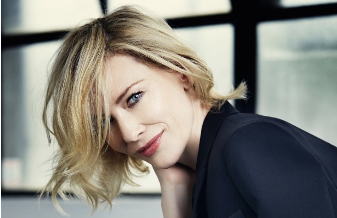
\includegraphics[width=\linewidth,height=0.092\textheight,keepaspectratio]{pic/demo_original.png}\\[-0.08em]
          原图
        \end{minipage}\hfill
        \begin{minipage}[t]{0.485\linewidth}
          \centering
          
\includegraphics[width=\linewidth,height=0.092\textheight,keepaspectratio]{pic/demo_sam_mask.png}\\[-0.08em]
          粗分割结果
        \end{minipage}
        \vspace{0.06em}

        \begin{minipage}[t]{0.485\linewidth}
          \centering
          
\includegraphics[width=\linewidth,height=0.092\textheight,keepaspectratio]{pic/demo_zim_alpha.png}\\[-0.08em]
          精细 alpha
        \end{minipage}\hfill
        \begin{minipage}[t]{0.485\linewidth}
          \centering
          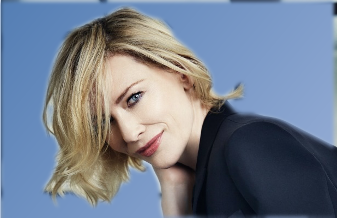
\includegraphics[width=\linewidth,height=0.092\textheight,keepaspectratio]{pic/demo_composite.png}\\[-0.08em]
          背景替换结果
        \end{minipage}
        \vspace{0.06em}

        从左上到右下：输入图像、SAM 粗分割、精细 alpha、换背景结果。
      \end{block}
  \end{columns}
\end{frame}

\section{问题定义}
\begin{frame}[t]{2. 任务流程与关键挑战}
  \footnotesize
  \linespread{0.94}\selectfont
  \begin{columns}[t,onlytextwidth]
    \column{0.55\textwidth}
      \begin{block}{输入输出流程与 Trimap}
        \centering
        \resizebox{0.98\linewidth}{!}{%
        \begin{tikzpicture}[node distance=0.6cm]
          \node[flow, minimum width=2.35cm, minimum height=0.92cm] (inp) {\textbf{图像 / 视频}\\文本提示};
          \node[warn, minimum width=1.95cm, minimum height=0.92cm, right=of inp] (sam) {\textbf{SAM 粗分割}\\文本驱动定位};
          \node[good, minimum width=1.75cm, minimum height=0.92cm, right=of sam] (zim) {\textbf{ZIM alpha}\\精细边界估计};
          \node[accent, minimum width=2.4cm, minimum height=0.92cm, right=of zim] (out) {\textbf{RGBA / 换背景}\\\textbf{/ 视频合成}};
          \draw[arr] (inp) -- (sam);
          \draw[arr] (sam) -- (zim);
          \draw[arr] (zim) -- (out);
        \end{tikzpicture}}

        \vspace{0.5em}
        \raggedright\scriptsize 先 \hilite{粗定位}，再把二值 mask 细化为 \hilite{软 alpha}；图像输出 $\alpha^\star$ / RGBA / 换背景图，视频输出逐帧 alpha 与合成视频。

        \vspace{0.7em}
        \centering
        \resizebox{0.8\linewidth}{!}{%
        
\begin{tikzpicture}[x=1cm,y=1cm]
          \fill[black] (0,0) rectangle (1.7,0.8);
          \fill[black!45] (1.7,0) rectangle (4.0,0.8);
          \fill[white] (4.0,0) rectangle (5.7,0.8);
          \draw[black!55, thick] (0,0) rectangle (5.7,0.8);
          \draw[black!55, thick] (1.7,0) -- (1.7,0.8);
          \draw[black!55, thick] (4.0,0) -- (4.0,0.8);
        \end{tikzpicture}}
        \par\vspace{0.2em}
        {\scriptsize Trimap —— 黑：背景 \quad 灰：不确定边界 \quad 白：前景}
      \end{block}
    \column{0.45\textwidth}
      \begin{block}{关键挑战与策略}
        \begin{itemize}
          \setlength{\itemsep}{0.55em}
          \item \textbf{开放词汇定位：}目标不只限于人，也含宠物、商品、玻璃杯等；
          \item \textbf{精细边界：}头发、毛发、半透明、细结构都不是硬二值边界；
          \item \textbf{零训练限制：}不能依赖大量 GPU 重新训练；
          \item \textbf{视频稳定性：}要避免 $\alpha$ 抖动与边界闪烁。
        \end{itemize}

        \vspace{0.6em}
        \textbf{策略：}不训练大模型，复用开源推理链路并自研 \hilite{边界优化与时序平滑}，形成 \hilite{定位—alpha—合成} 闭环。
      \end{block}
  \end{columns}
\end{frame}

\section{方法实现}
\begin{frame}[t]{3. 相关模块与系统动机}
  \footnotesize
  \linespread{0.92}\selectfont
  \begin{columns}[t,onlytextwidth]
    \column{0.33\textwidth}
      \begin{block}{A. 开放词汇粗分割}
        \centering
        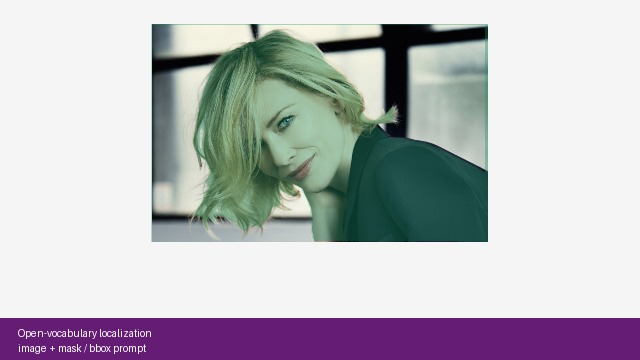
\includegraphics[width=0.92\linewidth,height=0.095\textheight,keepaspectratio]{pic/ext/grounded_sam_2_intro.jpg}

        \scriptsize
        SAM2 / SAM3 / Grounded-SAM-2 负责 \hilite{目标定位与初始分割}，为后续 bbox / points 提供入口。
      \end{block}
    \column{0.33\textwidth}
      \begin{block}{B. 图像 Matting}
        \centering
        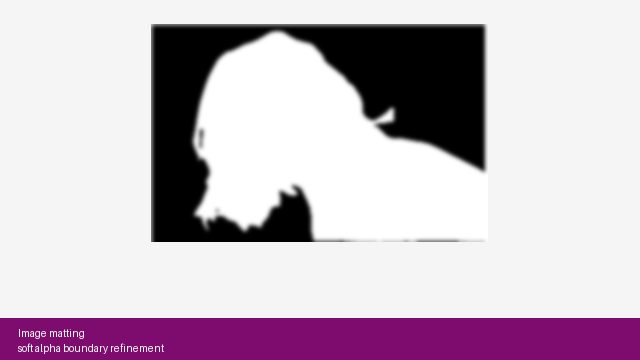
\includegraphics[width=0.92\linewidth,height=0.095\textheight,keepaspectratio]{pic/ext/teaser_arxiv_v2.png}

        \scriptsize
        ZIM 作为最终图像 matting 主线，将粗定位细化为 \hilite{软 alpha}；MAM 仅作为相关方法参考。
      \end{block}
    \column{0.34\textwidth}
      \begin{block}{C. 视频与应用}
        \centering
        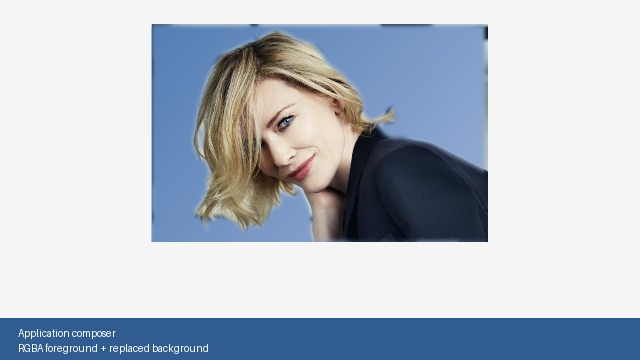
\includegraphics[width=0.92\linewidth,height=0.095\textheight,keepaspectratio]{pic/ext/matanyone2_teaser.jpg}

        \scriptsize
        MatAnyone2 用于 \hilite{人像视频 matting}；OpenCV 支持背景替换与背景虚化，作为系统应用展示。
      \end{block}
  \end{columns}
  \vspace{0.1em}

  \begin{block}{系统串联逻辑}
    \scriptsize
    A、B、C 依次回答“\hilite{目标是谁、在哪}”“\hilite{边界是否够精细}”“\hilite{系统能否演示}”：A 提供稳定的 bbox / points 入口，B 输出可合成的软 alpha，C 延伸到视频合成与背景替换；最终三者串联，并补充 \hilite{候选 mask 选择}、\hilite{边界优化} 与 \hilite{时序稳定} 等工程模块。
  \end{block}
\end{frame}

\begin{frame}[t]{4. 系统实现与方法总览}
  \footnotesize
  \linespread{0.91}\selectfont
  \begin{block}{总体流程}
    \centering
    \resizebox{0.95\linewidth}{!}{%
    \begin{tikzpicture}[
      node distance=4mm and 4mm,
      open/.style={rounded corners=2pt, draw=black!45, thick, fill=black!3, align=center, inner sep=4pt},
      ours/.style={rounded corners=2pt, draw=nankai!90!black, very thick, fill=nankai!14, align=center, inner sep=4pt},
      tag/.style={font=\bfseries\small, text=nankai}
    ]
      \node[tag, anchor=west] at (-0.2,1.55) {主线：图像文本分支};

      \node[open, minimum width=1.5cm, minimum height=0.88cm] (text) at (0,0.55) {文本\\提示};
      \node[open, right=of text, minimum width=1.9cm, minimum height=0.88cm] (sam) {SAM2 / SAM3\\Grounded-SAM-2};
      \node[open, right=of sam, minimum width=1.35cm, minimum height=0.88cm] (cand) {Candidate\\Masks};
      \node[ours, right=of cand, minimum width=1.95cm, minimum height=0.88cm] (rerank) {Prompt Ensemble\\+ Mask Rerank};
      \node[ours, right=of rerank, minimum width=1.9cm, minimum height=0.88cm] (auto) {Auto bbox/points\\+ trimap};
      \node[open, right=of auto, minimum width=1.35cm, minimum height=0.88cm] (mat) {ZIM\\alpha};
      \node[ours, right=of mat, minimum width=1.95cm, minimum height=0.88cm] (fusion) {Flip TTA + GF\\+ BSP};
      \node[ours, right=of fusion, minimum width=1.9cm, minimum height=0.88cm] (compose) {RGBA / Blur BG\\ / Replace BG};

      \draw[arr] (text) -- (sam);
      \draw[arr] (sam) -- (cand);
      \draw[arr] (cand) -- (rerank);
      \draw[arr] (rerank) -- (auto);
      \draw[arr] (auto) -- (mat);
      \draw[arr] (mat) -- (fusion);
      \draw[arr] (fusion) -- (compose);

      \node[tag, anchor=west] at (2.25,-0.9) {视频支线：首帧结果驱动时序一致性};
      \node[open, minimum width=1.75cm, minimum height=0.88cm] (ff) at (2.35,-1.9) {First-frame Mask\\from image branch};
      \node[open, right=of ff, minimum width=1.45cm, minimum height=0.88cm] (matany) {MatAnyone2};
      \node[open, right=of matany, minimum width=1.45cm, minimum height=0.88cm] (avideo) {Alpha\\Video};
      \node[ours, right=of avideo, minimum width=1.9cm, minimum height=0.88cm] (ts) {Boundary-only\\Temporal Smoothing};
      \node[ours, right=of ts, minimum width=1.75cm, minimum height=0.88cm] (vcomp) {Video\\Composition};

      \draw[arr,densely dashed] (fusion.south) |- (ff.north);
      \draw[arr] (ff) -- (matany);
      \draw[arr] (matany) -- (avideo);
      \draw[arr] (avideo) -- (ts);
      \draw[arr] (ts) -- (vcomp);
    \end{tikzpicture}}

    \vspace{0.15em}
    {\scriptsize 灰框表示开源模型或现成推理模块，紫框表示团队自研模块；Flip TTA + GF + BSP 对应 ZIM 精细抠图优化链路。}
  \end{block}

  \vspace{-0.3em}
  \begin{block}{团队实现模块与最终目标}
    \scriptsize
    \textbf{团队自研模块：}
    \texttt{prompt\_ensemble.py}、\texttt{mask\_rerank.py}、\texttt{auto\_prompt.py / trimap.py}

    \texttt{final\_claim\_pipeline.py}、\texttt{box\_prior\_pipeline.py}、\texttt{composer\_demo.py}、\texttt{temporal\_smooth.py}

    \vspace{0.05em}
    \textbf{最终实现目标：}
    保持 \hilite{zero-training} 设定，整合粗定位、精细 alpha、背景编辑与视频稳定，并在 MicroMat official-prompt 评估中验证 ZIM 后端优化。
  \end{block}
\end{frame}

% ===== 队友占位章节：上游开放词汇分割（史傅冠华）=====
% ============================================================================
%  队友章节：上游开放词汇分割   ——   负责人：史傅冠华
% ----------------------------------------------------------------------------
%  · 本文件由主文件 slides.tex 通过 % ============================================================================
%  队友章节：上游开放词汇分割   ——   负责人：史傅冠华
% ----------------------------------------------------------------------------
%  · 本文件由主文件 slides.tex 通过 % ============================================================================
%  队友章节：上游开放词汇分割   ——   负责人：史傅冠华
% ----------------------------------------------------------------------------
%  · 本文件由主文件 slides.tex 通过 \input{sections/sam.tex} 引入，
%    继承主文件导言区的全部宏 / 配色 / 字体，无需自带 \documentclass 或 \begin{document}。
%  · 内容：模型选型 → Prompt Ensemble + Rerank → 多尺度融合 + 消融 → 可视化
% ============================================================================
\section{上游分割}

% ==================== 第 1 页：模型选型与系统定位 ====================
\begin{frame}[t]{1. 上游模型选型：为什么用 SAM2？}
  \footnotesize
  \linespread{0.90}\selectfont

  \begin{columns}[T,onlytextwidth]
    \column{0.50\textwidth}
      \tcard{softorange}{2.00cm}{定位需求分析}{%
        \textbf{系统需求：}给定图像，输出 bbox / points，供 ZIM 做精细 matting。\\
        \textbf{关键约束：}
        \begin{itemize}
          \setlength{\itemsep}{0.02em}
          \item \hilite{zero-training} — 不微调模型参数；
          \item 推理高效 — 单卡秒级；
          \item bbox prompt 原生支持 — 与下游接口统一。
        \end{itemize}
        \vspace{0.02em}
        \textbf{不选 SAM3：}模型更大、推理慢约 2--3 倍，bbox-only 提升有限。\\
        \textbf{不选 Grounded-SAM-2：}额外引入 text encoder，增加显存开销。
      }
    \column{0.50\textwidth}
      \tcard{accentblue}{2.00cm}{SAM2 适配性}{%
        \begin{itemize}
          \setlength{\itemsep}{0.04em}
          \item \textbf{Hiera 架构} — 轻量高效，Hiera-Base+ 仅 80.8M 参数；
          \item \textbf{native bbox + points} — 无需适配层；
          \item \textbf{多候选 mask + IoU 评分} — 为 rerank 提供置信度；
          \item \textbf{实测性能} — A10 上约 1.16 it/s（bbox-only）；
          \item 社区活跃，checkpoint 可下载。
        \end{itemize}
      }
  \end{columns}

  \vspace{0.15em}
  \notestrip{accentblue}{\centering\scriptsize
  \textbf{定位：}SAM2 负责回答 \hilite{``目标在哪''} — 输出 bbox + points + 候选 mask；精细软 alpha 留给下游 ZIM + TTA-GF + BSP。}
\end{frame}

% ==================== 第 2 页：Prompt Ensemble + Mask Rerank ====================
\begin{frame}[t]{2. 核心优化一：Prompt Ensemble 与 IoU 引导重排序}
  \scriptsize
  \linespread{0.90}\selectfont

  \notestrip{deepred}{\tiny
  \textbf{动机：}SAM2 单次 bbox 推理易受局部纹理干扰，可能选到次优 mask。我们提出 \hilite{Prompt Ensemble + IoU 引导重排序}：多组 prompt 策略生成候选 mask，再利用 SAM2 内置 IoU 与结构先验选出最优。}

  \vspace{0.35em}
  \centering
  \resizebox{0.92\linewidth}{!}{%
  \begin{tikzpicture}[
    x=1cm, y=1cm,
    >={Latex[length=2.5mm,width=2mm]},
    every node/.style={font=\tiny},
    softsh/.style={blur shadow={shadow blur steps=5, shadow xshift=0.4pt,
                   shadow yshift=-0.5pt, shadow opacity=24, shadow blur radius=1.5pt}},
    nodebase/.style={softsh, rounded corners=3pt, line width=0.9pt, align=center, inner sep=3pt},
    io/.style={nodebase, draw=black!50, fill=black!5, minimum width=1.5cm, minimum height=0.58cm},
    sam/.style={nodebase, draw=accentblue!82!black, fill=accentblue!14, minimum width=1.55cm, minimum height=0.58cm},
    cand/.style={nodebase, draw=softorange!72!black, fill=softorange!12, minimum width=1.2cm, minimum height=0.58cm},
    ours/.style={nodebase, draw=nankai!88!black, fill=nankai!14, minimum width=1.35cm, minimum height=0.58cm},
    best/.style={nodebase, draw=softgreen!72!black, fill=softgreen!16, minimum width=1.35cm, minimum height=0.58cm,
                 line width=1.2pt},
    pipe/.style={-{Latex[length=2.4mm,width=2mm]}, line width=1pt, draw=nankai!80!black, rounded corners=2pt},
    tag/.style={font=\tiny\bfseries, text=nankai!88!black}
  ]
    % ---- top branch ----
    \node[io]   (img)  at (0,1.15) {\textbf{原图 + bbox}};
    \node[sam]  (sam0) at (2.2,1.15) {\textbf{SAM2}\\[0.5pt]{\tiny bbox-only}};
    \node[cand] (c0)   at (4.2,1.15) {\tiny 3 candidates};

    % ---- bottom branch ----
    \node[io]   (img2) at (0,0) {\textbf{原图 + bbox}\\[0.5pt]{\tiny + positive points}};
    \node[sam]  (sam1) at (2.2,0) {\textbf{SAM2}\\[0.5pt]{\tiny bbox + pos}};
    \node[cand] (c1)   at (4.2,0) {\tiny up to 3 candidates};

    % ---- merge into rerank ----
    \node[ours] (rerank) at (6.3,0.575) {\textbf{Ensemble}\\[0.5pt]{\tiny + Rerank}};
    \node[best] (out)    at (8.3,0.575) {\textbf{最优 mask}\\[0.5pt]{\tiny $\alpha$}};

    % ---- arrows ----
    \draw[pipe] (img)  -- (sam0);
    \draw[pipe] (sam0) -- (c0);
    \draw[pipe] (img2) -- (sam1);
    \draw[pipe] (sam1) -- (c1);
    \draw[pipe] (c0.east) -| (rerank.north);
    \draw[pipe] (c1.east) -| (rerank.south);
    \draw[pipe] (rerank) -- (out);

    % ---- grouping bands ----
    \begin{scope}[on background layer]
      \node[fit=(img)(sam0)(c0)(img2)(sam1)(c1), rounded corners=6pt,
            draw=accentblue!45, line width=0.8pt, fill=accentblue!5, inner sep=8pt] (grpA) {};
      \node[fit=(rerank)(out), rounded corners=6pt,
            draw=nankai!52, line width=0.8pt, fill=nankai!6, inner sep=8pt] (grpB) {};
    \end{scope}
    \node[tag, anchor=south west] at ([xshift=6pt,yshift=-1pt]grpA.north west)
      {多策略候选生成 · Multi-prompt generation};
    \node[tag, anchor=south east] at ([xshift=-6pt,yshift=-1pt]grpB.north east)
      {置信度重排序 · Confidence-aware rerank};
  \end{tikzpicture}}

  \vspace{0.04em}
  \begin{columns}[T,onlytextwidth]
    \column{0.24\textwidth}
      \ccard{nankai}{0.95cm}{%
      {\fontsize{6}{7}\selectfont\textbf{\textcolor{nankai!88!black}{重排序公式}}}\\[1pt]
      {\fontsize{5.5}{6.5}\selectfont $S(m)=0.55\cdot\text{IoU}(m)+0.25\cdot\text{conn}(m)+0.20\cdot\text{bbox\_cov}(m)$}}
    \column{0.25\textwidth}
      \ccard{accentblue}{0.95cm}{%
      {\fontsize{6}{7}\selectfont\textbf{\textcolor{accentblue!85!black}{SAM2 IoU (55\%)}}}\\[1pt]
      {\fontsize{5.5}{6.5}\selectfont 模型自身的 mask 质量置信度；最可靠信号}}
    \column{0.25\textwidth}
      \ccard{softorange}{0.95cm}{%
      {\fontsize{6}{7}\selectfont\textbf{\textcolor{softorange!75!black}{连通性 (25\%)}}}\\[1pt]
      {\fontsize{5.5}{6.5}\selectfont 连通分量数衡量 mask 碎片化；惩罚零散碎片}}
    \column{0.26\textwidth}
      \ccard{softgreen}{0.95cm}{%
      {\fontsize{6}{7}\selectfont\textbf{\textcolor{softgreen!60!black}{bbox 覆盖 (20\%)}}}\\[1pt]
      {\fontsize{5.5}{6.5}\selectfont mask 应填充 bbox 的 10--70\%；偏离的压低}}
  \end{columns}
\end{frame}

% ==================== 第 3 页：多尺度推理 ====================
\begin{frame}[t]{3. 核心优化二：多尺度推理}
  \scriptsize
  \linespread{0.92}\selectfont

  \notestrip{deepred}{\scriptsize
  \textbf{动机：}单尺度 SAM2 推理对图像分辨率敏感，边界处可能产生偏差。我们引入 \hilite{多尺度推理}：在多个尺度分别运行 SAM2，融合结果以降低单尺度偏差。}

  \vspace{0.70em}
  \begin{columns}[T,onlytextwidth]
    \column{0.50\textwidth}
      \tcard{accentblue}{3.20cm}{多尺度推理原理}{%
        \begin{itemize}
          \setlength{\itemsep}{0.08em}
          \item 在 3 个尺度 $\{0.75\times, 1.0\times, 1.25\times\}$ 分别运行 SAM2；
          \item 将各尺度 mask resize 回原图分辨率；
          \item 平均融合：$\alpha_{\text{fused}}=\frac{1}{3}\sum_{s}\alpha_s$；
          \item 单一尺度的边界偏差被多数投票稀释；
          \item 不增加模型参数，纯推理时后处理。
        \end{itemize}
        \vspace{0.10em}
        \textbf{与 Ensemble 叠加：}\hilite{每尺度各自 ensemble rerank}，再跨尺度平均 —— 两阶段互补，进一步提升鲁棒性。}
    \column{0.50\textwidth}
      \tcard{nankai}{3.20cm}{直观理解}{%
        \begin{itemize}
          \setlength{\itemsep}{0.10em}
          \item \textbf{放大（1.25×）：}捕捉更精细的边界细节；
          \item \textbf{原始（1.0×）：}保持模型训练分布下的最优精度；
          \item \textbf{缩小（0.75×）：}获得更大感受野，减少局部歧义。
        \end{itemize}
        \vspace{0.15em}
        三个尺度的 mask 经 resize + 平均后，\hilite{单尺度的随机偏差被平滑}，类似集成学习中 bagging 的思路。

        \vspace{0.12em}
        \textbf{代价：}推理时间约 $\times$3（3 个尺度），但与 ensemble 组合时收益大于开销。}
  \end{columns}
\end{frame}

% ==================== 第 4 页：消融实验设定 ====================
\begin{frame}[t]{4. 消融实验设定}
  \footnotesize
  \linespread{0.92}\selectfont

  \begin{columns}[T,onlytextwidth]
    \column{0.48\textwidth}
      \tcard{softgray}{2.60cm}{数据集与模型}{%
        \begin{itemize}
          \setlength{\itemsep}{0.08em}
          \item \textbf{数据集：}MicroMat-3K valid706 子集
          \begin{itemize}
            \item 706 张图像，64 张基础图像
            \item 每张配有 official bbox + GT alpha
          \end{itemize}
          \item \textbf{模型：}SAM2.1 Hiera-Base+（80.8M 参数）
        \end{itemize}
      }
      \vspace{0.15em}
      \tcard{accentblue}{1.90cm}{评测指标}{%
        \begin{itemize}
          \setlength{\itemsep}{0.06em}
          \item \textbf{SAD}（Sum of Absolute Differences）—— 绝对误差总和
          \item \textbf{MSE} —— 均方误差
          \item \textbf{MAE$\times$1000} —— 平均绝对误差（$\times$1000）
          \item \textbf{Boundary SAD} —— 边界带（5px）SAD，衡量边缘质量
        \end{itemize}
      }
    \column{0.52\textwidth}
      \tcard{nankai}{4.65cm}{消融方法设计（8 种组合）}{%
        \textbf{核心思路：}控制变量法，逐项检验各部分贡献。
        \vspace{0.08em}
        \begin{itemize}
          \setlength{\itemsep}{0.05em}
          \item \textbf{bbox\_binary} — 基线：bbox-only 单次推理 + 硬二值化
          \item \textbf{+ guided} — 单路 + guided filter 边缘平滑
          \item \textbf{+ multiscale} — 单路 + 3 尺度融合
          \item \textbf{+ multiscale\_guided} — 单路 + 多尺度 + guided
          \item \textbf{+ ensemble\_rerank} — 双 prompt 候选 + IoU 重排序
          \item \textbf{+ ensemble\_guided} — ensemble + guided
          \item \textbf{+ ensemble\_multiscale} — ensemble + 多尺度
          \item \textbf{+ ensemble\_multiscale\_guided} — 全部叠加
        \end{itemize}
        \vspace{0.08em}
        从 1 到 8 逐步叠加优化，分析各模块的\hilite{独立贡献与交互效应}。}
  \end{columns}
\end{frame}

% ==================== 第 5 页：消融结果 ====================
\begin{frame}[t]{5. 消融实验结果（valid706）}
  \scriptsize
  \linespread{0.92}\selectfont

  \begin{columns}[T,onlytextwidth]
    \column{0.58\textwidth}
      \begin{block}{完整消融对比表}
        \vspace{-0.3em}
        \centering
        {\fontsize{7}{8}\selectfont
        \setlength{\tabcolsep}{2.2pt}
        \renewcommand{\arraystretch}{1.04}
        \resizebox{0.99\linewidth}{!}{%
        \begin{tabular}{lrrrr}
          \toprule
          \textbf{方法} & \textbf{SAD $\downarrow$} & \textbf{MSE $\downarrow$} & \textbf{MAE$\times$1000 $\downarrow$} & \textbf{Bnd-SAD $\downarrow$} \\
          \midrule
          \textbf{ensemble\_guided (最终)} & \textbf{2774.0} & \textbf{0.000747} & \textbf{0.981} & \textbf{1215.5} \\
          ensemble\_multiscale\_guided & 2915.4 & 0.000742 & 1.033 & 1188.8 \\
          ensemble\_rerank & 2930.9 & 0.000843 & 1.037 & 1380.1 \\
          ensemble\_multiscale & 2997.4 & 0.000796 & 1.062 & 1279.2 \\
          multiscale\_guided & 3145.3 & 0.000828 & 1.089 & 1249.0 \\
          guided & 3161.9 & 0.000845 & 1.095 & 1271.2 \\
          multiscale & 3228.3 & 0.000894 & 1.119 & 1340.7 \\
          \textbf{bbox\_binary (基线)} & \textbf{3313.5} & \textbf{0.000956} & \textbf{1.149} & \textbf{1431.5} \\
          \bottomrule
        \end{tabular}}}
      \end{block}
    \column{0.42\textwidth}
      \tcard{softgreen}{2.05cm}{关键发现}{%
        \begin{itemize}
          \setlength{\itemsep}{0.08em}
          \item \hilite{Ensemble rerank 单点最有效}（SAD$\downarrow$11.5\% vs 基线）
          \item Guided filter 对 Boundary 改善显著（1432$\to$1271）
          \item Multiscale 单独增益有限（3313$\to$3228）
          \item 三者叠加达最优：SAD$\downarrow$16.3\%，MAE$\downarrow$14.6\%
        \end{itemize}
      }

      \vspace{0.25em}
      \tcard{nankai}{1.30cm}{最终提交方法}{%
        \centering
        Ensemble Rerank + Guided Filter}

      \vspace{0.6em}
      \begin{columns}[T,onlytextwidth]
        \column{0.33\textwidth}
          \metricchip{softgreen}{SAD 改善{\tiny\ (vs 基线)}}{$-16.3\%$}
        \column{0.33\textwidth}
          \metricchip{softgreen}{MAE 改善{\tiny\ (vs 基线)}}{$-14.6\%$}
        \column{0.34\textwidth}
          \metricchip{nankai}{Boundary 改善{\tiny\ (vs 基线)}}{$-15.1\%$}
      \end{columns}
  \end{columns}
\end{frame}

% ==================== 第 6 页：可视化案例一 ====================
\begin{frame}[t]{6. 可视化案例一：大型目标（汽车）}
  \footnotesize
  \linespread{0.92}\selectfont

  \vspace{-0.2em}
  \centering
  \fcolorbox{black!25}{white}{%
    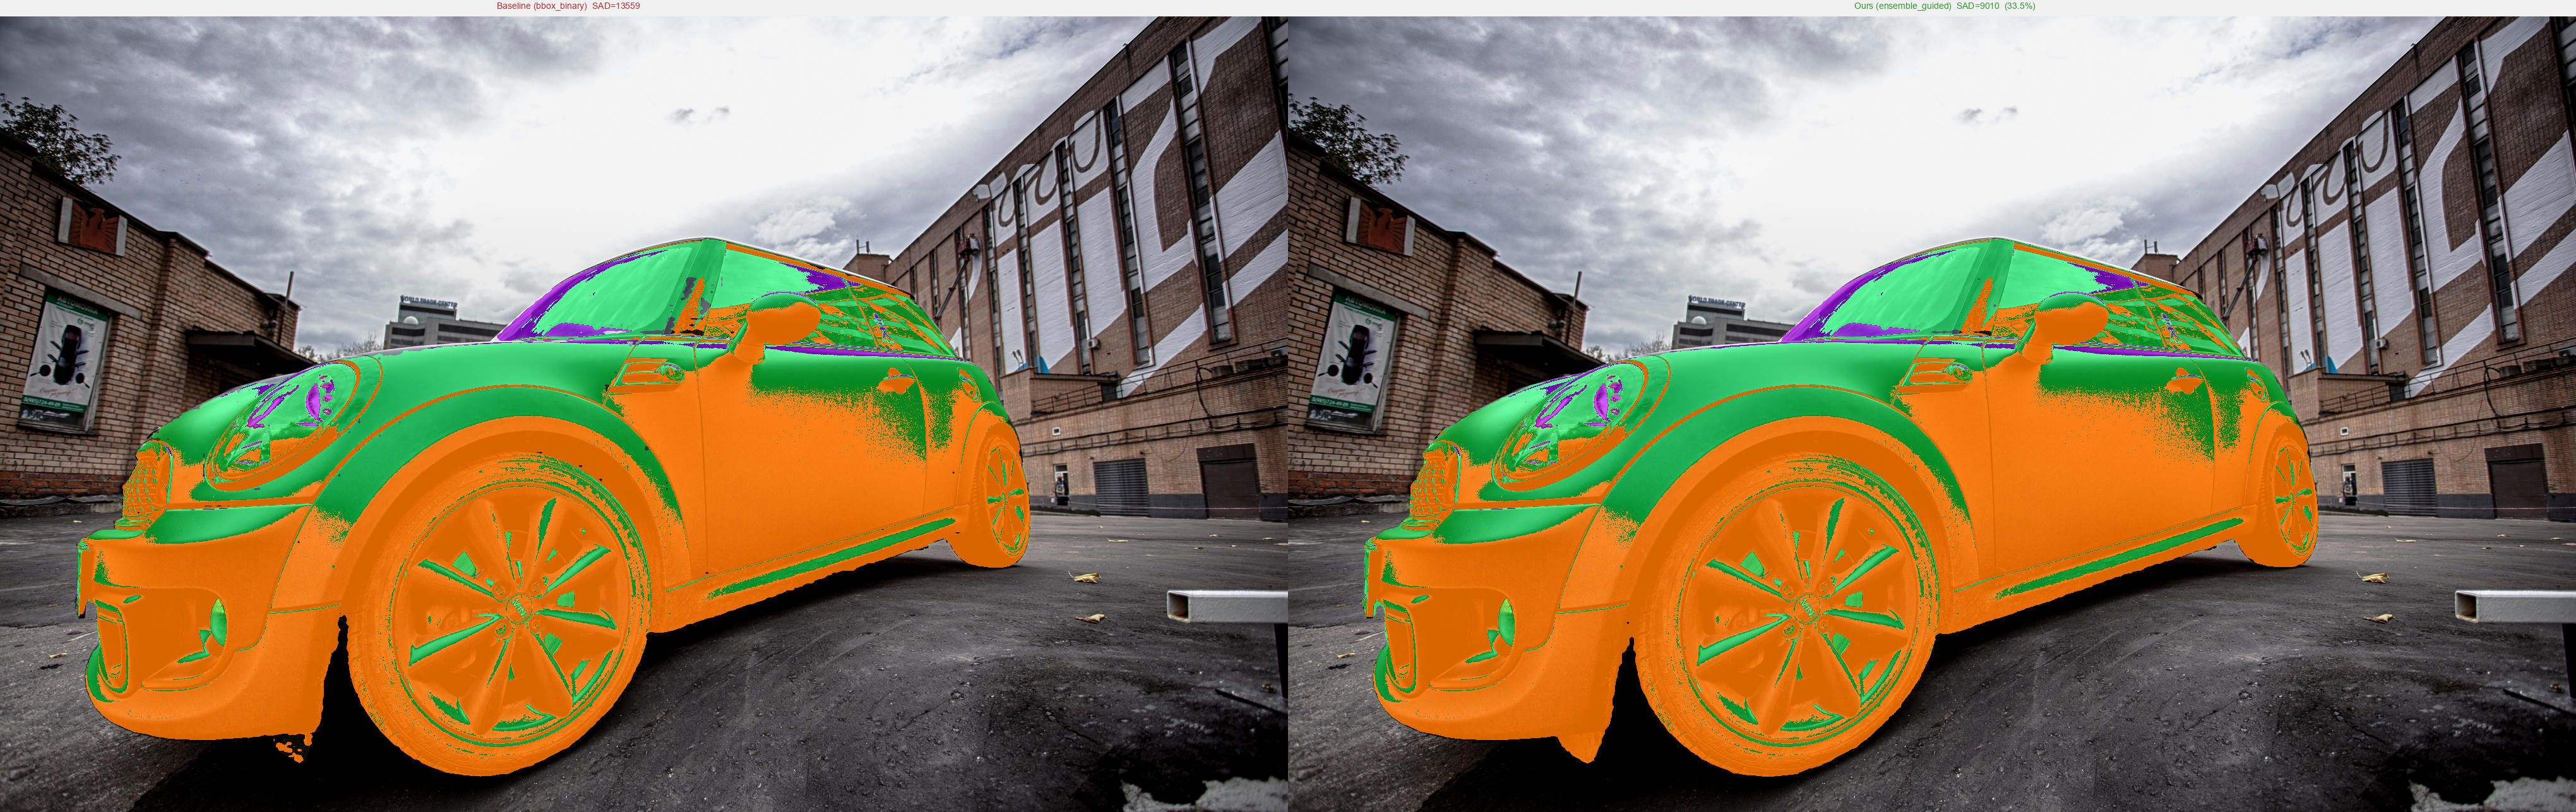
\includegraphics[width=0.92\linewidth,height=0.60\textheight,keepaspectratio]{pic/sam2_case1_compare.png}}

  \vspace{0.12em}
  \begin{columns}[T,onlytextwidth]
    \column{0.50\textwidth}
      \tcard{deepred}{1.10cm}{Baseline 问题}{%
        \small SAD=13559。车轮和车窗边缘有明显的 mask 溢出，导致前景区域偏大。}
    \column{0.50\textwidth}
      \tcard{softgreen}{1.10cm}{优化后改善}{%
        \small SAD=9010（$\downarrow$33.5\%）。边界更贴合车身轮廓，车窗和轮毂区域 mask 精度提升。}
  \end{columns}
\end{frame}

% ==================== 第 7 页：可视化案例二 ====================
\begin{frame}[t]{7. 可视化案例二：小型目标}
  \footnotesize
  \linespread{0.92}\selectfont

  \vspace{-0.2em}
  \centering
  \fcolorbox{black!25}{white}{%
    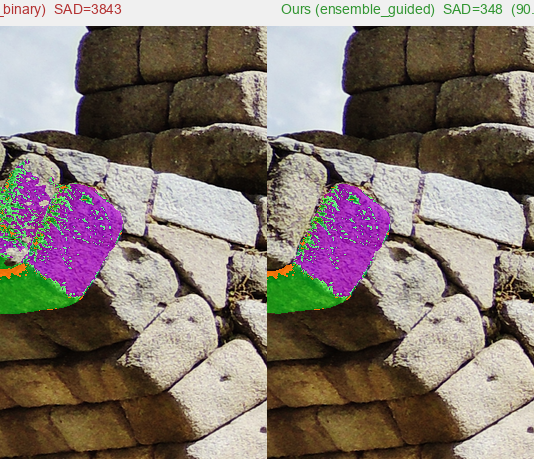
\includegraphics[width=0.80\linewidth,height=0.60\textheight,keepaspectratio]{pic/sam2_case2_compare.png}}

  \vspace{0.12em}
  \begin{columns}[T,onlytextwidth]
    \column{0.50\textwidth}
      \tcard{deepred}{1.10cm}{Baseline 问题}{%
        \small SAD=3843。微小目标（bbox 仅 117$\times$133）容易误选背景区域，mask 几乎全错。}
    \column{0.50\textwidth}
      \tcard{softgreen}{1.10cm}{优化后改善}{%
        \small SAD=348（$\downarrow$90.9\%）。Ensemble 重排序有效纠正了候选选择错误，精确捕获目标。}
  \end{columns}
\end{frame}

% ==================== 第 8 页：可视化案例三 ====================
\begin{frame}[t]{8. 可视化案例三：细结构物体}
  \footnotesize
  \linespread{0.92}\selectfont

  \vspace{-0.2em}
  \centering
  \fcolorbox{black!25}{white}{%
    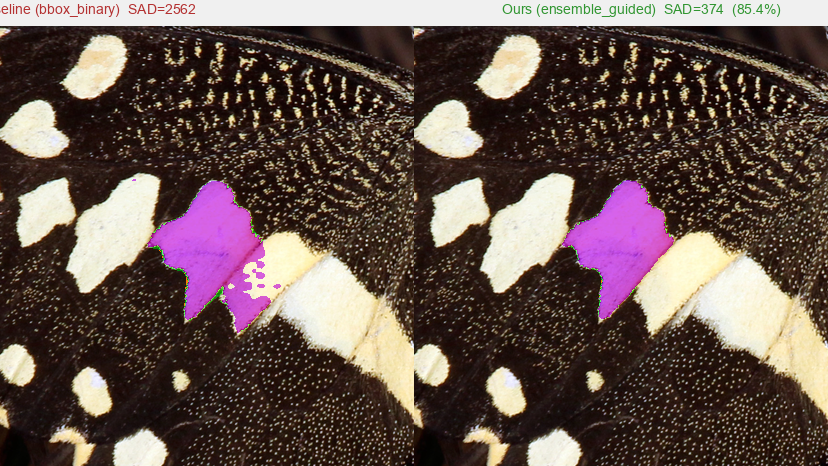
\includegraphics[width=0.80\linewidth,height=0.60\textheight,keepaspectratio]{pic/sam2_case3_compare.png}}

  \vspace{0.12em}
  \begin{columns}[T,onlytextwidth]
    \column{0.50\textwidth}
      \tcard{deepred}{1.10cm}{Baseline 问题}{%
        \small SAD=2562。细结构处有 mask 碎片和空洞，边界不完整。}
    \column{0.50\textwidth}
      \tcard{softgreen}{1.10cm}{优化后改善}{%
        \small SAD=374（$\downarrow$85.4\%）。Mask 更完整，碎片显著减少，细边缘更清晰。}
  \end{columns}
\end{frame}

% ---- 本节结束 ----
 引入，
%    继承主文件导言区的全部宏 / 配色 / 字体，无需自带 \documentclass 或 \begin{document}。
%  · 内容：模型选型 → Prompt Ensemble + Rerank → 多尺度融合 + 消融 → 可视化
% ============================================================================
\section{上游分割}

% ==================== 第 1 页：模型选型与系统定位 ====================
\begin{frame}[t]{1. 上游模型选型：为什么用 SAM2？}
  \footnotesize
  \linespread{0.90}\selectfont

  \begin{columns}[T,onlytextwidth]
    \column{0.50\textwidth}
      \tcard{softorange}{2.00cm}{定位需求分析}{%
        \textbf{系统需求：}给定图像，输出 bbox / points，供 ZIM 做精细 matting。\\
        \textbf{关键约束：}
        \begin{itemize}
          \setlength{\itemsep}{0.02em}
          \item \hilite{zero-training} — 不微调模型参数；
          \item 推理高效 — 单卡秒级；
          \item bbox prompt 原生支持 — 与下游接口统一。
        \end{itemize}
        \vspace{0.02em}
        \textbf{不选 SAM3：}模型更大、推理慢约 2--3 倍，bbox-only 提升有限。\\
        \textbf{不选 Grounded-SAM-2：}额外引入 text encoder，增加显存开销。
      }
    \column{0.50\textwidth}
      \tcard{accentblue}{2.00cm}{SAM2 适配性}{%
        \begin{itemize}
          \setlength{\itemsep}{0.04em}
          \item \textbf{Hiera 架构} — 轻量高效，Hiera-Base+ 仅 80.8M 参数；
          \item \textbf{native bbox + points} — 无需适配层；
          \item \textbf{多候选 mask + IoU 评分} — 为 rerank 提供置信度；
          \item \textbf{实测性能} — A10 上约 1.16 it/s（bbox-only）；
          \item 社区活跃，checkpoint 可下载。
        \end{itemize}
      }
  \end{columns}

  \vspace{0.15em}
  \notestrip{accentblue}{\centering\scriptsize
  \textbf{定位：}SAM2 负责回答 \hilite{``目标在哪''} — 输出 bbox + points + 候选 mask；精细软 alpha 留给下游 ZIM + TTA-GF + BSP。}
\end{frame}

% ==================== 第 2 页：Prompt Ensemble + Mask Rerank ====================
\begin{frame}[t]{2. 核心优化一：Prompt Ensemble 与 IoU 引导重排序}
  \scriptsize
  \linespread{0.90}\selectfont

  \notestrip{deepred}{\tiny
  \textbf{动机：}SAM2 单次 bbox 推理易受局部纹理干扰，可能选到次优 mask。我们提出 \hilite{Prompt Ensemble + IoU 引导重排序}：多组 prompt 策略生成候选 mask，再利用 SAM2 内置 IoU 与结构先验选出最优。}

  \vspace{0.35em}
  \centering
  \resizebox{0.92\linewidth}{!}{%
  \begin{tikzpicture}[
    x=1cm, y=1cm,
    >={Latex[length=2.5mm,width=2mm]},
    every node/.style={font=\tiny},
    softsh/.style={blur shadow={shadow blur steps=5, shadow xshift=0.4pt,
                   shadow yshift=-0.5pt, shadow opacity=24, shadow blur radius=1.5pt}},
    nodebase/.style={softsh, rounded corners=3pt, line width=0.9pt, align=center, inner sep=3pt},
    io/.style={nodebase, draw=black!50, fill=black!5, minimum width=1.5cm, minimum height=0.58cm},
    sam/.style={nodebase, draw=accentblue!82!black, fill=accentblue!14, minimum width=1.55cm, minimum height=0.58cm},
    cand/.style={nodebase, draw=softorange!72!black, fill=softorange!12, minimum width=1.2cm, minimum height=0.58cm},
    ours/.style={nodebase, draw=nankai!88!black, fill=nankai!14, minimum width=1.35cm, minimum height=0.58cm},
    best/.style={nodebase, draw=softgreen!72!black, fill=softgreen!16, minimum width=1.35cm, minimum height=0.58cm,
                 line width=1.2pt},
    pipe/.style={-{Latex[length=2.4mm,width=2mm]}, line width=1pt, draw=nankai!80!black, rounded corners=2pt},
    tag/.style={font=\tiny\bfseries, text=nankai!88!black}
  ]
    % ---- top branch ----
    \node[io]   (img)  at (0,1.15) {\textbf{原图 + bbox}};
    \node[sam]  (sam0) at (2.2,1.15) {\textbf{SAM2}\\[0.5pt]{\tiny bbox-only}};
    \node[cand] (c0)   at (4.2,1.15) {\tiny 3 candidates};

    % ---- bottom branch ----
    \node[io]   (img2) at (0,0) {\textbf{原图 + bbox}\\[0.5pt]{\tiny + positive points}};
    \node[sam]  (sam1) at (2.2,0) {\textbf{SAM2}\\[0.5pt]{\tiny bbox + pos}};
    \node[cand] (c1)   at (4.2,0) {\tiny up to 3 candidates};

    % ---- merge into rerank ----
    \node[ours] (rerank) at (6.3,0.575) {\textbf{Ensemble}\\[0.5pt]{\tiny + Rerank}};
    \node[best] (out)    at (8.3,0.575) {\textbf{最优 mask}\\[0.5pt]{\tiny $\alpha$}};

    % ---- arrows ----
    \draw[pipe] (img)  -- (sam0);
    \draw[pipe] (sam0) -- (c0);
    \draw[pipe] (img2) -- (sam1);
    \draw[pipe] (sam1) -- (c1);
    \draw[pipe] (c0.east) -| (rerank.north);
    \draw[pipe] (c1.east) -| (rerank.south);
    \draw[pipe] (rerank) -- (out);

    % ---- grouping bands ----
    \begin{scope}[on background layer]
      \node[fit=(img)(sam0)(c0)(img2)(sam1)(c1), rounded corners=6pt,
            draw=accentblue!45, line width=0.8pt, fill=accentblue!5, inner sep=8pt] (grpA) {};
      \node[fit=(rerank)(out), rounded corners=6pt,
            draw=nankai!52, line width=0.8pt, fill=nankai!6, inner sep=8pt] (grpB) {};
    \end{scope}
    \node[tag, anchor=south west] at ([xshift=6pt,yshift=-1pt]grpA.north west)
      {多策略候选生成 · Multi-prompt generation};
    \node[tag, anchor=south east] at ([xshift=-6pt,yshift=-1pt]grpB.north east)
      {置信度重排序 · Confidence-aware rerank};
  \end{tikzpicture}}

  \vspace{0.04em}
  \begin{columns}[T,onlytextwidth]
    \column{0.24\textwidth}
      \ccard{nankai}{0.95cm}{%
      {\fontsize{6}{7}\selectfont\textbf{\textcolor{nankai!88!black}{重排序公式}}}\\[1pt]
      {\fontsize{5.5}{6.5}\selectfont $S(m)=0.55\cdot\text{IoU}(m)+0.25\cdot\text{conn}(m)+0.20\cdot\text{bbox\_cov}(m)$}}
    \column{0.25\textwidth}
      \ccard{accentblue}{0.95cm}{%
      {\fontsize{6}{7}\selectfont\textbf{\textcolor{accentblue!85!black}{SAM2 IoU (55\%)}}}\\[1pt]
      {\fontsize{5.5}{6.5}\selectfont 模型自身的 mask 质量置信度；最可靠信号}}
    \column{0.25\textwidth}
      \ccard{softorange}{0.95cm}{%
      {\fontsize{6}{7}\selectfont\textbf{\textcolor{softorange!75!black}{连通性 (25\%)}}}\\[1pt]
      {\fontsize{5.5}{6.5}\selectfont 连通分量数衡量 mask 碎片化；惩罚零散碎片}}
    \column{0.26\textwidth}
      \ccard{softgreen}{0.95cm}{%
      {\fontsize{6}{7}\selectfont\textbf{\textcolor{softgreen!60!black}{bbox 覆盖 (20\%)}}}\\[1pt]
      {\fontsize{5.5}{6.5}\selectfont mask 应填充 bbox 的 10--70\%；偏离的压低}}
  \end{columns}
\end{frame}

% ==================== 第 3 页：多尺度推理 ====================
\begin{frame}[t]{3. 核心优化二：多尺度推理}
  \scriptsize
  \linespread{0.92}\selectfont

  \notestrip{deepred}{\scriptsize
  \textbf{动机：}单尺度 SAM2 推理对图像分辨率敏感，边界处可能产生偏差。我们引入 \hilite{多尺度推理}：在多个尺度分别运行 SAM2，融合结果以降低单尺度偏差。}

  \vspace{0.70em}
  \begin{columns}[T,onlytextwidth]
    \column{0.50\textwidth}
      \tcard{accentblue}{3.20cm}{多尺度推理原理}{%
        \begin{itemize}
          \setlength{\itemsep}{0.08em}
          \item 在 3 个尺度 $\{0.75\times, 1.0\times, 1.25\times\}$ 分别运行 SAM2；
          \item 将各尺度 mask resize 回原图分辨率；
          \item 平均融合：$\alpha_{\text{fused}}=\frac{1}{3}\sum_{s}\alpha_s$；
          \item 单一尺度的边界偏差被多数投票稀释；
          \item 不增加模型参数，纯推理时后处理。
        \end{itemize}
        \vspace{0.10em}
        \textbf{与 Ensemble 叠加：}\hilite{每尺度各自 ensemble rerank}，再跨尺度平均 —— 两阶段互补，进一步提升鲁棒性。}
    \column{0.50\textwidth}
      \tcard{nankai}{3.20cm}{直观理解}{%
        \begin{itemize}
          \setlength{\itemsep}{0.10em}
          \item \textbf{放大（1.25×）：}捕捉更精细的边界细节；
          \item \textbf{原始（1.0×）：}保持模型训练分布下的最优精度；
          \item \textbf{缩小（0.75×）：}获得更大感受野，减少局部歧义。
        \end{itemize}
        \vspace{0.15em}
        三个尺度的 mask 经 resize + 平均后，\hilite{单尺度的随机偏差被平滑}，类似集成学习中 bagging 的思路。

        \vspace{0.12em}
        \textbf{代价：}推理时间约 $\times$3（3 个尺度），但与 ensemble 组合时收益大于开销。}
  \end{columns}
\end{frame}

% ==================== 第 4 页：消融实验设定 ====================
\begin{frame}[t]{4. 消融实验设定}
  \footnotesize
  \linespread{0.92}\selectfont

  \begin{columns}[T,onlytextwidth]
    \column{0.48\textwidth}
      \tcard{softgray}{2.60cm}{数据集与模型}{%
        \begin{itemize}
          \setlength{\itemsep}{0.08em}
          \item \textbf{数据集：}MicroMat-3K valid706 子集
          \begin{itemize}
            \item 706 张图像，64 张基础图像
            \item 每张配有 official bbox + GT alpha
          \end{itemize}
          \item \textbf{模型：}SAM2.1 Hiera-Base+（80.8M 参数）
        \end{itemize}
      }
      \vspace{0.15em}
      \tcard{accentblue}{1.90cm}{评测指标}{%
        \begin{itemize}
          \setlength{\itemsep}{0.06em}
          \item \textbf{SAD}（Sum of Absolute Differences）—— 绝对误差总和
          \item \textbf{MSE} —— 均方误差
          \item \textbf{MAE$\times$1000} —— 平均绝对误差（$\times$1000）
          \item \textbf{Boundary SAD} —— 边界带（5px）SAD，衡量边缘质量
        \end{itemize}
      }
    \column{0.52\textwidth}
      \tcard{nankai}{4.65cm}{消融方法设计（8 种组合）}{%
        \textbf{核心思路：}控制变量法，逐项检验各部分贡献。
        \vspace{0.08em}
        \begin{itemize}
          \setlength{\itemsep}{0.05em}
          \item \textbf{bbox\_binary} — 基线：bbox-only 单次推理 + 硬二值化
          \item \textbf{+ guided} — 单路 + guided filter 边缘平滑
          \item \textbf{+ multiscale} — 单路 + 3 尺度融合
          \item \textbf{+ multiscale\_guided} — 单路 + 多尺度 + guided
          \item \textbf{+ ensemble\_rerank} — 双 prompt 候选 + IoU 重排序
          \item \textbf{+ ensemble\_guided} — ensemble + guided
          \item \textbf{+ ensemble\_multiscale} — ensemble + 多尺度
          \item \textbf{+ ensemble\_multiscale\_guided} — 全部叠加
        \end{itemize}
        \vspace{0.08em}
        从 1 到 8 逐步叠加优化，分析各模块的\hilite{独立贡献与交互效应}。}
  \end{columns}
\end{frame}

% ==================== 第 5 页：消融结果 ====================
\begin{frame}[t]{5. 消融实验结果（valid706）}
  \scriptsize
  \linespread{0.92}\selectfont

  \begin{columns}[T,onlytextwidth]
    \column{0.58\textwidth}
      \begin{block}{完整消融对比表}
        \vspace{-0.3em}
        \centering
        {\fontsize{7}{8}\selectfont
        \setlength{\tabcolsep}{2.2pt}
        \renewcommand{\arraystretch}{1.04}
        \resizebox{0.99\linewidth}{!}{%
        \begin{tabular}{lrrrr}
          \toprule
          \textbf{方法} & \textbf{SAD $\downarrow$} & \textbf{MSE $\downarrow$} & \textbf{MAE$\times$1000 $\downarrow$} & \textbf{Bnd-SAD $\downarrow$} \\
          \midrule
          \textbf{ensemble\_guided (最终)} & \textbf{2774.0} & \textbf{0.000747} & \textbf{0.981} & \textbf{1215.5} \\
          ensemble\_multiscale\_guided & 2915.4 & 0.000742 & 1.033 & 1188.8 \\
          ensemble\_rerank & 2930.9 & 0.000843 & 1.037 & 1380.1 \\
          ensemble\_multiscale & 2997.4 & 0.000796 & 1.062 & 1279.2 \\
          multiscale\_guided & 3145.3 & 0.000828 & 1.089 & 1249.0 \\
          guided & 3161.9 & 0.000845 & 1.095 & 1271.2 \\
          multiscale & 3228.3 & 0.000894 & 1.119 & 1340.7 \\
          \textbf{bbox\_binary (基线)} & \textbf{3313.5} & \textbf{0.000956} & \textbf{1.149} & \textbf{1431.5} \\
          \bottomrule
        \end{tabular}}}
      \end{block}
    \column{0.42\textwidth}
      \tcard{softgreen}{2.05cm}{关键发现}{%
        \begin{itemize}
          \setlength{\itemsep}{0.08em}
          \item \hilite{Ensemble rerank 单点最有效}（SAD$\downarrow$11.5\% vs 基线）
          \item Guided filter 对 Boundary 改善显著（1432$\to$1271）
          \item Multiscale 单独增益有限（3313$\to$3228）
          \item 三者叠加达最优：SAD$\downarrow$16.3\%，MAE$\downarrow$14.6\%
        \end{itemize}
      }

      \vspace{0.25em}
      \tcard{nankai}{1.30cm}{最终提交方法}{%
        \centering
        Ensemble Rerank + Guided Filter}

      \vspace{0.6em}
      \begin{columns}[T,onlytextwidth]
        \column{0.33\textwidth}
          \metricchip{softgreen}{SAD 改善{\tiny\ (vs 基线)}}{$-16.3\%$}
        \column{0.33\textwidth}
          \metricchip{softgreen}{MAE 改善{\tiny\ (vs 基线)}}{$-14.6\%$}
        \column{0.34\textwidth}
          \metricchip{nankai}{Boundary 改善{\tiny\ (vs 基线)}}{$-15.1\%$}
      \end{columns}
  \end{columns}
\end{frame}

% ==================== 第 6 页：可视化案例一 ====================
\begin{frame}[t]{6. 可视化案例一：大型目标（汽车）}
  \footnotesize
  \linespread{0.92}\selectfont

  \vspace{-0.2em}
  \centering
  \fcolorbox{black!25}{white}{%
    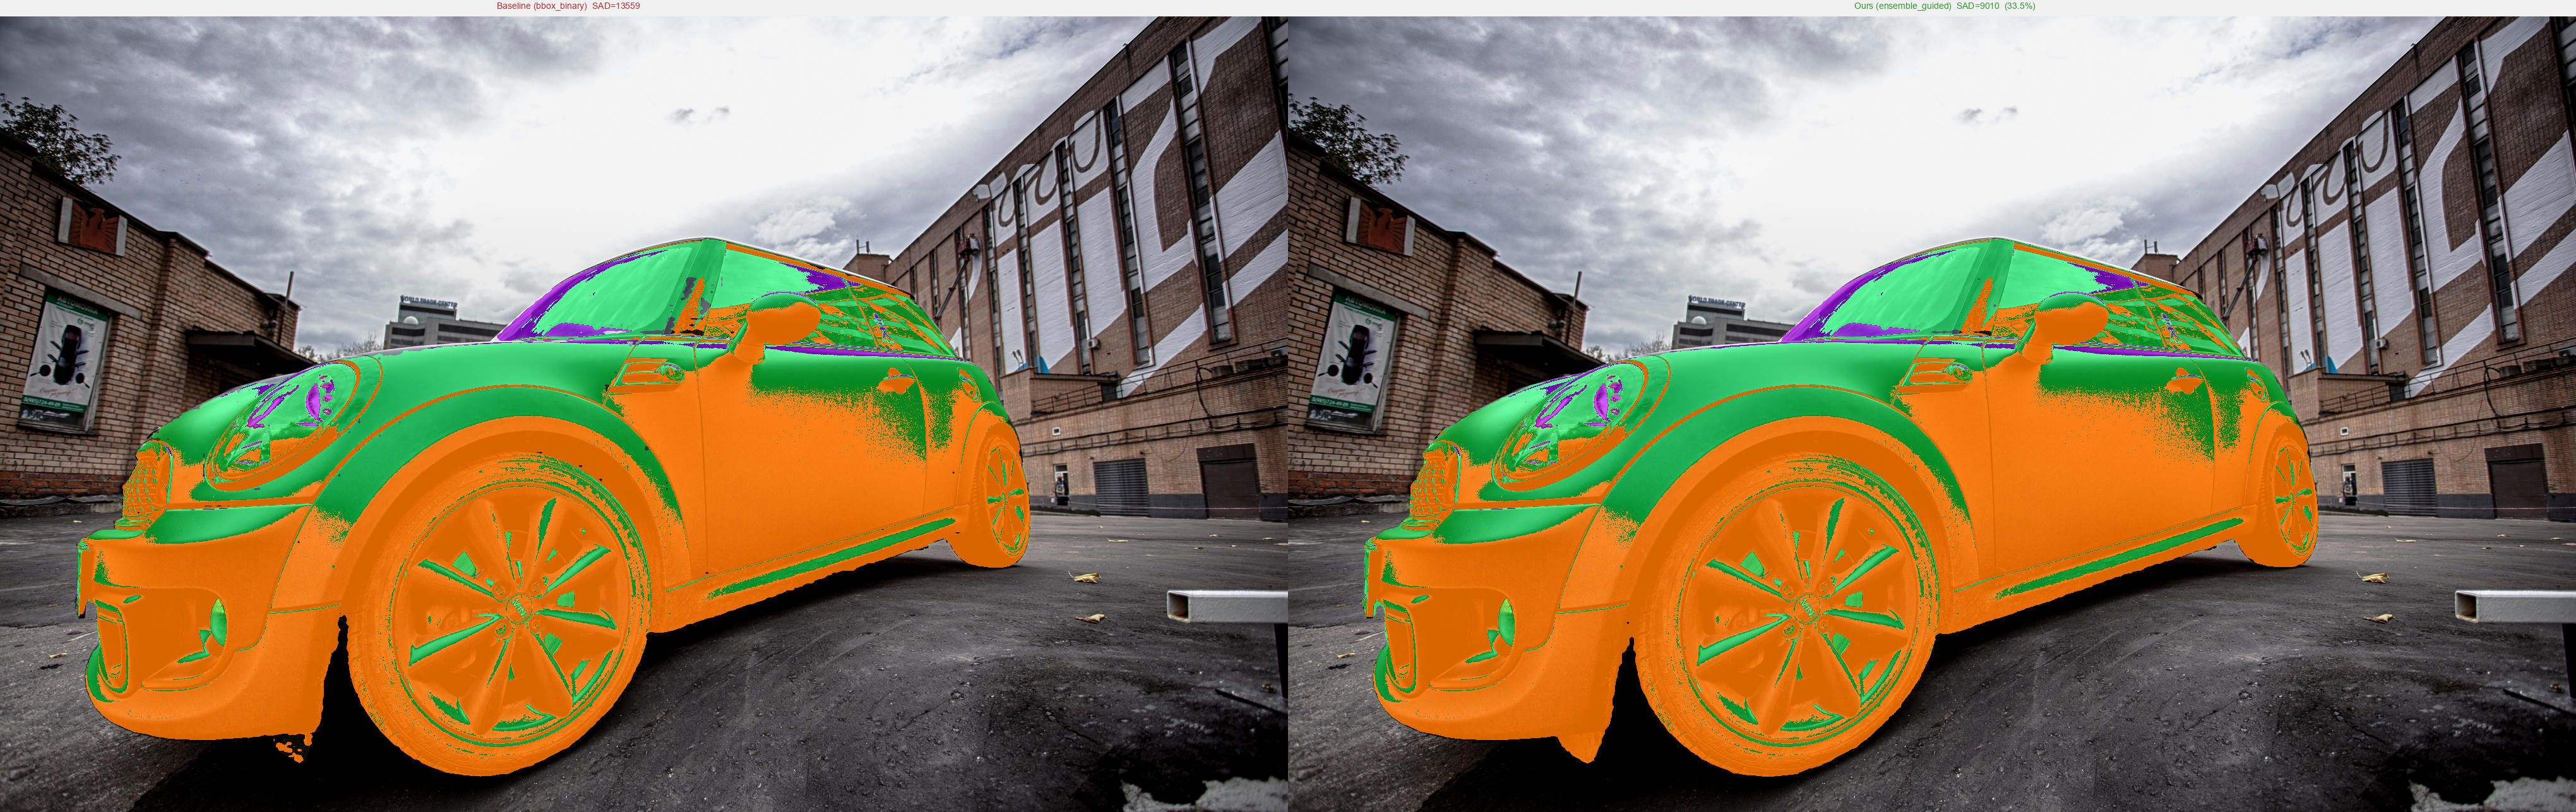
\includegraphics[width=0.92\linewidth,height=0.60\textheight,keepaspectratio]{pic/sam2_case1_compare.png}}

  \vspace{0.12em}
  \begin{columns}[T,onlytextwidth]
    \column{0.50\textwidth}
      \tcard{deepred}{1.10cm}{Baseline 问题}{%
        \small SAD=13559。车轮和车窗边缘有明显的 mask 溢出，导致前景区域偏大。}
    \column{0.50\textwidth}
      \tcard{softgreen}{1.10cm}{优化后改善}{%
        \small SAD=9010（$\downarrow$33.5\%）。边界更贴合车身轮廓，车窗和轮毂区域 mask 精度提升。}
  \end{columns}
\end{frame}

% ==================== 第 7 页：可视化案例二 ====================
\begin{frame}[t]{7. 可视化案例二：小型目标}
  \footnotesize
  \linespread{0.92}\selectfont

  \vspace{-0.2em}
  \centering
  \fcolorbox{black!25}{white}{%
    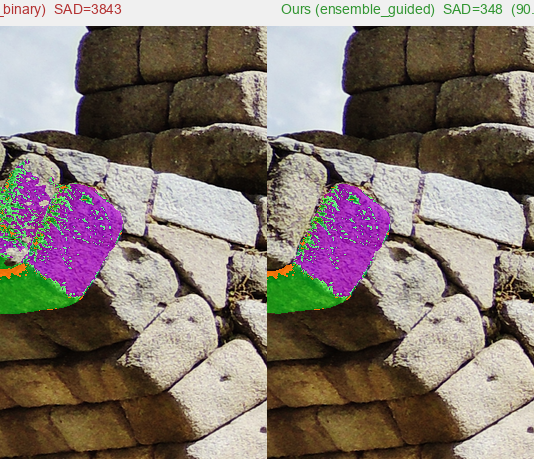
\includegraphics[width=0.80\linewidth,height=0.60\textheight,keepaspectratio]{pic/sam2_case2_compare.png}}

  \vspace{0.12em}
  \begin{columns}[T,onlytextwidth]
    \column{0.50\textwidth}
      \tcard{deepred}{1.10cm}{Baseline 问题}{%
        \small SAD=3843。微小目标（bbox 仅 117$\times$133）容易误选背景区域，mask 几乎全错。}
    \column{0.50\textwidth}
      \tcard{softgreen}{1.10cm}{优化后改善}{%
        \small SAD=348（$\downarrow$90.9\%）。Ensemble 重排序有效纠正了候选选择错误，精确捕获目标。}
  \end{columns}
\end{frame}

% ==================== 第 8 页：可视化案例三 ====================
\begin{frame}[t]{8. 可视化案例三：细结构物体}
  \footnotesize
  \linespread{0.92}\selectfont

  \vspace{-0.2em}
  \centering
  \fcolorbox{black!25}{white}{%
    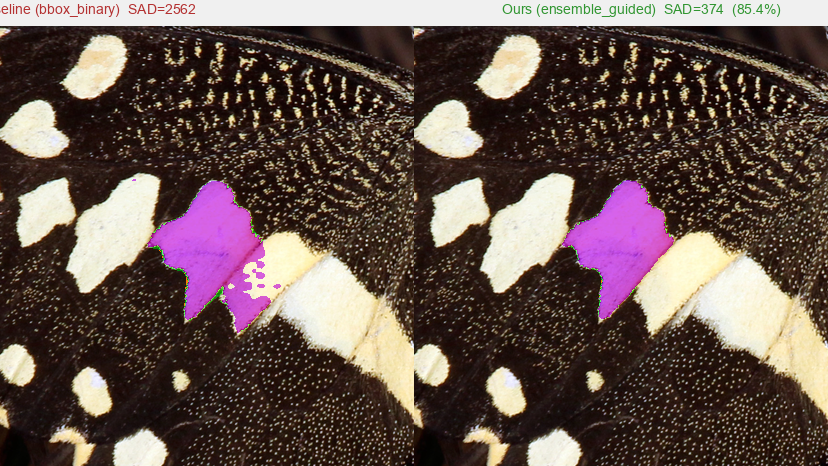
\includegraphics[width=0.80\linewidth,height=0.60\textheight,keepaspectratio]{pic/sam2_case3_compare.png}}

  \vspace{0.12em}
  \begin{columns}[T,onlytextwidth]
    \column{0.50\textwidth}
      \tcard{deepred}{1.10cm}{Baseline 问题}{%
        \small SAD=2562。细结构处有 mask 碎片和空洞，边界不完整。}
    \column{0.50\textwidth}
      \tcard{softgreen}{1.10cm}{优化后改善}{%
        \small SAD=374（$\downarrow$85.4\%）。Mask 更完整，碎片显著减少，细边缘更清晰。}
  \end{columns}
\end{frame}

% ---- 本节结束 ----
 引入，
%    继承主文件导言区的全部宏 / 配色 / 字体，无需自带 \documentclass 或 \begin{document}。
%  · 内容：模型选型 → Prompt Ensemble + Rerank → 多尺度融合 + 消融 → 可视化
% ============================================================================
\section{上游分割}

% ==================== 第 1 页：模型选型与系统定位 ====================
\begin{frame}[t]{1. 上游模型选型：为什么用 SAM2？}
  \footnotesize
  \linespread{0.90}\selectfont

  \begin{columns}[T,onlytextwidth]
    \column{0.50\textwidth}
      \tcard{softorange}{2.00cm}{定位需求分析}{%
        \textbf{系统需求：}给定图像，输出 bbox / points，供 ZIM 做精细 matting。\\
        \textbf{关键约束：}
        \begin{itemize}
          \setlength{\itemsep}{0.02em}
          \item \hilite{zero-training} — 不微调模型参数；
          \item 推理高效 — 单卡秒级；
          \item bbox prompt 原生支持 — 与下游接口统一。
        \end{itemize}
        \vspace{0.02em}
        \textbf{不选 SAM3：}模型更大、推理慢约 2--3 倍，bbox-only 提升有限。\\
        \textbf{不选 Grounded-SAM-2：}额外引入 text encoder，增加显存开销。
      }
    \column{0.50\textwidth}
      \tcard{accentblue}{2.00cm}{SAM2 适配性}{%
        \begin{itemize}
          \setlength{\itemsep}{0.04em}
          \item \textbf{Hiera 架构} — 轻量高效，Hiera-Base+ 仅 80.8M 参数；
          \item \textbf{native bbox + points} — 无需适配层；
          \item \textbf{多候选 mask + IoU 评分} — 为 rerank 提供置信度；
          \item \textbf{实测性能} — A10 上约 1.16 it/s（bbox-only）；
          \item 社区活跃，checkpoint 可下载。
        \end{itemize}
      }
  \end{columns}

  \vspace{0.15em}
  \notestrip{accentblue}{\centering\scriptsize
  \textbf{定位：}SAM2 负责回答 \hilite{``目标在哪''} — 输出 bbox + points + 候选 mask；精细软 alpha 留给下游 ZIM + TTA-GF + BSP。}
\end{frame}

% ==================== 第 2 页：Prompt Ensemble + Mask Rerank ====================
\begin{frame}[t]{2. 核心优化一：Prompt Ensemble 与 IoU 引导重排序}
  \scriptsize
  \linespread{0.90}\selectfont

  \notestrip{deepred}{\tiny
  \textbf{动机：}SAM2 单次 bbox 推理易受局部纹理干扰，可能选到次优 mask。我们提出 \hilite{Prompt Ensemble + IoU 引导重排序}：多组 prompt 策略生成候选 mask，再利用 SAM2 内置 IoU 与结构先验选出最优。}

  \vspace{0.35em}
  \centering
  \resizebox{0.92\linewidth}{!}{%
  \begin{tikzpicture}[
    x=1cm, y=1cm,
    >={Latex[length=2.5mm,width=2mm]},
    every node/.style={font=\tiny},
    softsh/.style={blur shadow={shadow blur steps=5, shadow xshift=0.4pt,
                   shadow yshift=-0.5pt, shadow opacity=24, shadow blur radius=1.5pt}},
    nodebase/.style={softsh, rounded corners=3pt, line width=0.9pt, align=center, inner sep=3pt},
    io/.style={nodebase, draw=black!50, fill=black!5, minimum width=1.5cm, minimum height=0.58cm},
    sam/.style={nodebase, draw=accentblue!82!black, fill=accentblue!14, minimum width=1.55cm, minimum height=0.58cm},
    cand/.style={nodebase, draw=softorange!72!black, fill=softorange!12, minimum width=1.2cm, minimum height=0.58cm},
    ours/.style={nodebase, draw=nankai!88!black, fill=nankai!14, minimum width=1.35cm, minimum height=0.58cm},
    best/.style={nodebase, draw=softgreen!72!black, fill=softgreen!16, minimum width=1.35cm, minimum height=0.58cm,
                 line width=1.2pt},
    pipe/.style={-{Latex[length=2.4mm,width=2mm]}, line width=1pt, draw=nankai!80!black, rounded corners=2pt},
    tag/.style={font=\tiny\bfseries, text=nankai!88!black}
  ]
    % ---- top branch ----
    \node[io]   (img)  at (0,1.15) {\textbf{原图 + bbox}};
    \node[sam]  (sam0) at (2.2,1.15) {\textbf{SAM2}\\[0.5pt]{\tiny bbox-only}};
    \node[cand] (c0)   at (4.2,1.15) {\tiny 3 candidates};

    % ---- bottom branch ----
    \node[io]   (img2) at (0,0) {\textbf{原图 + bbox}\\[0.5pt]{\tiny + positive points}};
    \node[sam]  (sam1) at (2.2,0) {\textbf{SAM2}\\[0.5pt]{\tiny bbox + pos}};
    \node[cand] (c1)   at (4.2,0) {\tiny up to 3 candidates};

    % ---- merge into rerank ----
    \node[ours] (rerank) at (6.3,0.575) {\textbf{Ensemble}\\[0.5pt]{\tiny + Rerank}};
    \node[best] (out)    at (8.3,0.575) {\textbf{最优 mask}\\[0.5pt]{\tiny $\alpha$}};

    % ---- arrows ----
    \draw[pipe] (img)  -- (sam0);
    \draw[pipe] (sam0) -- (c0);
    \draw[pipe] (img2) -- (sam1);
    \draw[pipe] (sam1) -- (c1);
    \draw[pipe] (c0.east) -| (rerank.north);
    \draw[pipe] (c1.east) -| (rerank.south);
    \draw[pipe] (rerank) -- (out);

    % ---- grouping bands ----
    \begin{scope}[on background layer]
      \node[fit=(img)(sam0)(c0)(img2)(sam1)(c1), rounded corners=6pt,
            draw=accentblue!45, line width=0.8pt, fill=accentblue!5, inner sep=8pt] (grpA) {};
      \node[fit=(rerank)(out), rounded corners=6pt,
            draw=nankai!52, line width=0.8pt, fill=nankai!6, inner sep=8pt] (grpB) {};
    \end{scope}
    \node[tag, anchor=south west] at ([xshift=6pt,yshift=-1pt]grpA.north west)
      {多策略候选生成 · Multi-prompt generation};
    \node[tag, anchor=south east] at ([xshift=-6pt,yshift=-1pt]grpB.north east)
      {置信度重排序 · Confidence-aware rerank};
  \end{tikzpicture}}

  \vspace{0.04em}
  \begin{columns}[T,onlytextwidth]
    \column{0.24\textwidth}
      \ccard{nankai}{0.95cm}{%
      {\fontsize{6}{7}\selectfont\textbf{\textcolor{nankai!88!black}{重排序公式}}}\\[1pt]
      {\fontsize{5.5}{6.5}\selectfont $S(m)=0.55\cdot\text{IoU}(m)+0.25\cdot\text{conn}(m)+0.20\cdot\text{bbox\_cov}(m)$}}
    \column{0.25\textwidth}
      \ccard{accentblue}{0.95cm}{%
      {\fontsize{6}{7}\selectfont\textbf{\textcolor{accentblue!85!black}{SAM2 IoU (55\%)}}}\\[1pt]
      {\fontsize{5.5}{6.5}\selectfont 模型自身的 mask 质量置信度；最可靠信号}}
    \column{0.25\textwidth}
      \ccard{softorange}{0.95cm}{%
      {\fontsize{6}{7}\selectfont\textbf{\textcolor{softorange!75!black}{连通性 (25\%)}}}\\[1pt]
      {\fontsize{5.5}{6.5}\selectfont 连通分量数衡量 mask 碎片化；惩罚零散碎片}}
    \column{0.26\textwidth}
      \ccard{softgreen}{0.95cm}{%
      {\fontsize{6}{7}\selectfont\textbf{\textcolor{softgreen!60!black}{bbox 覆盖 (20\%)}}}\\[1pt]
      {\fontsize{5.5}{6.5}\selectfont mask 应填充 bbox 的 10--70\%；偏离的压低}}
  \end{columns}
\end{frame}

% ==================== 第 3 页：多尺度推理 ====================
\begin{frame}[t]{3. 核心优化二：多尺度推理}
  \scriptsize
  \linespread{0.92}\selectfont

  \notestrip{deepred}{\scriptsize
  \textbf{动机：}单尺度 SAM2 推理对图像分辨率敏感，边界处可能产生偏差。我们引入 \hilite{多尺度推理}：在多个尺度分别运行 SAM2，融合结果以降低单尺度偏差。}

  \vspace{0.70em}
  \begin{columns}[T,onlytextwidth]
    \column{0.50\textwidth}
      \tcard{accentblue}{3.20cm}{多尺度推理原理}{%
        \begin{itemize}
          \setlength{\itemsep}{0.08em}
          \item 在 3 个尺度 $\{0.75\times, 1.0\times, 1.25\times\}$ 分别运行 SAM2；
          \item 将各尺度 mask resize 回原图分辨率；
          \item 平均融合：$\alpha_{\text{fused}}=\frac{1}{3}\sum_{s}\alpha_s$；
          \item 单一尺度的边界偏差被多数投票稀释；
          \item 不增加模型参数，纯推理时后处理。
        \end{itemize}
        \vspace{0.10em}
        \textbf{与 Ensemble 叠加：}\hilite{每尺度各自 ensemble rerank}，再跨尺度平均 —— 两阶段互补，进一步提升鲁棒性。}
    \column{0.50\textwidth}
      \tcard{nankai}{3.20cm}{直观理解}{%
        \begin{itemize}
          \setlength{\itemsep}{0.10em}
          \item \textbf{放大（1.25×）：}捕捉更精细的边界细节；
          \item \textbf{原始（1.0×）：}保持模型训练分布下的最优精度；
          \item \textbf{缩小（0.75×）：}获得更大感受野，减少局部歧义。
        \end{itemize}
        \vspace{0.15em}
        三个尺度的 mask 经 resize + 平均后，\hilite{单尺度的随机偏差被平滑}，类似集成学习中 bagging 的思路。

        \vspace{0.12em}
        \textbf{代价：}推理时间约 $\times$3（3 个尺度），但与 ensemble 组合时收益大于开销。}
  \end{columns}
\end{frame}

% ==================== 第 4 页：消融实验设定 ====================
\begin{frame}[t]{4. 消融实验设定}
  \footnotesize
  \linespread{0.92}\selectfont

  \begin{columns}[T,onlytextwidth]
    \column{0.48\textwidth}
      \tcard{softgray}{2.60cm}{数据集与模型}{%
        \begin{itemize}
          \setlength{\itemsep}{0.08em}
          \item \textbf{数据集：}MicroMat-3K valid706 子集
          \begin{itemize}
            \item 706 张图像，64 张基础图像
            \item 每张配有 official bbox + GT alpha
          \end{itemize}
          \item \textbf{模型：}SAM2.1 Hiera-Base+（80.8M 参数）
        \end{itemize}
      }
      \vspace{0.15em}
      \tcard{accentblue}{1.90cm}{评测指标}{%
        \begin{itemize}
          \setlength{\itemsep}{0.06em}
          \item \textbf{SAD}（Sum of Absolute Differences）—— 绝对误差总和
          \item \textbf{MSE} —— 均方误差
          \item \textbf{MAE$\times$1000} —— 平均绝对误差（$\times$1000）
          \item \textbf{Boundary SAD} —— 边界带（5px）SAD，衡量边缘质量
        \end{itemize}
      }
    \column{0.52\textwidth}
      \tcard{nankai}{4.65cm}{消融方法设计（8 种组合）}{%
        \textbf{核心思路：}控制变量法，逐项检验各部分贡献。
        \vspace{0.08em}
        \begin{itemize}
          \setlength{\itemsep}{0.05em}
          \item \textbf{bbox\_binary} — 基线：bbox-only 单次推理 + 硬二值化
          \item \textbf{+ guided} — 单路 + guided filter 边缘平滑
          \item \textbf{+ multiscale} — 单路 + 3 尺度融合
          \item \textbf{+ multiscale\_guided} — 单路 + 多尺度 + guided
          \item \textbf{+ ensemble\_rerank} — 双 prompt 候选 + IoU 重排序
          \item \textbf{+ ensemble\_guided} — ensemble + guided
          \item \textbf{+ ensemble\_multiscale} — ensemble + 多尺度
          \item \textbf{+ ensemble\_multiscale\_guided} — 全部叠加
        \end{itemize}
        \vspace{0.08em}
        从 1 到 8 逐步叠加优化，分析各模块的\hilite{独立贡献与交互效应}。}
  \end{columns}
\end{frame}

% ==================== 第 5 页：消融结果 ====================
\begin{frame}[t]{5. 消融实验结果（valid706）}
  \scriptsize
  \linespread{0.92}\selectfont

  \begin{columns}[T,onlytextwidth]
    \column{0.58\textwidth}
      \begin{block}{完整消融对比表}
        \vspace{-0.3em}
        \centering
        {\fontsize{7}{8}\selectfont
        \setlength{\tabcolsep}{2.2pt}
        \renewcommand{\arraystretch}{1.04}
        \resizebox{0.99\linewidth}{!}{%
        \begin{tabular}{lrrrr}
          \toprule
          \textbf{方法} & \textbf{SAD $\downarrow$} & \textbf{MSE $\downarrow$} & \textbf{MAE$\times$1000 $\downarrow$} & \textbf{Bnd-SAD $\downarrow$} \\
          \midrule
          \textbf{ensemble\_guided (最终)} & \textbf{2774.0} & \textbf{0.000747} & \textbf{0.981} & \textbf{1215.5} \\
          ensemble\_multiscale\_guided & 2915.4 & 0.000742 & 1.033 & 1188.8 \\
          ensemble\_rerank & 2930.9 & 0.000843 & 1.037 & 1380.1 \\
          ensemble\_multiscale & 2997.4 & 0.000796 & 1.062 & 1279.2 \\
          multiscale\_guided & 3145.3 & 0.000828 & 1.089 & 1249.0 \\
          guided & 3161.9 & 0.000845 & 1.095 & 1271.2 \\
          multiscale & 3228.3 & 0.000894 & 1.119 & 1340.7 \\
          \textbf{bbox\_binary (基线)} & \textbf{3313.5} & \textbf{0.000956} & \textbf{1.149} & \textbf{1431.5} \\
          \bottomrule
        \end{tabular}}}
      \end{block}
    \column{0.42\textwidth}
      \tcard{softgreen}{2.05cm}{关键发现}{%
        \begin{itemize}
          \setlength{\itemsep}{0.08em}
          \item \hilite{Ensemble rerank 单点最有效}（SAD$\downarrow$11.5\% vs 基线）
          \item Guided filter 对 Boundary 改善显著（1432$\to$1271）
          \item Multiscale 单独增益有限（3313$\to$3228）
          \item 三者叠加达最优：SAD$\downarrow$16.3\%，MAE$\downarrow$14.6\%
        \end{itemize}
      }

      \vspace{0.25em}
      \tcard{nankai}{1.30cm}{最终提交方法}{%
        \centering
        Ensemble Rerank + Guided Filter}

      \vspace{0.6em}
      \begin{columns}[T,onlytextwidth]
        \column{0.33\textwidth}
          \metricchip{softgreen}{SAD 改善{\tiny\ (vs 基线)}}{$-16.3\%$}
        \column{0.33\textwidth}
          \metricchip{softgreen}{MAE 改善{\tiny\ (vs 基线)}}{$-14.6\%$}
        \column{0.34\textwidth}
          \metricchip{nankai}{Boundary 改善{\tiny\ (vs 基线)}}{$-15.1\%$}
      \end{columns}
  \end{columns}
\end{frame}

% ==================== 第 6 页：可视化案例一 ====================
\begin{frame}[t]{6. 可视化案例一：大型目标（汽车）}
  \footnotesize
  \linespread{0.92}\selectfont

  \vspace{-0.2em}
  \centering
  \fcolorbox{black!25}{white}{%
    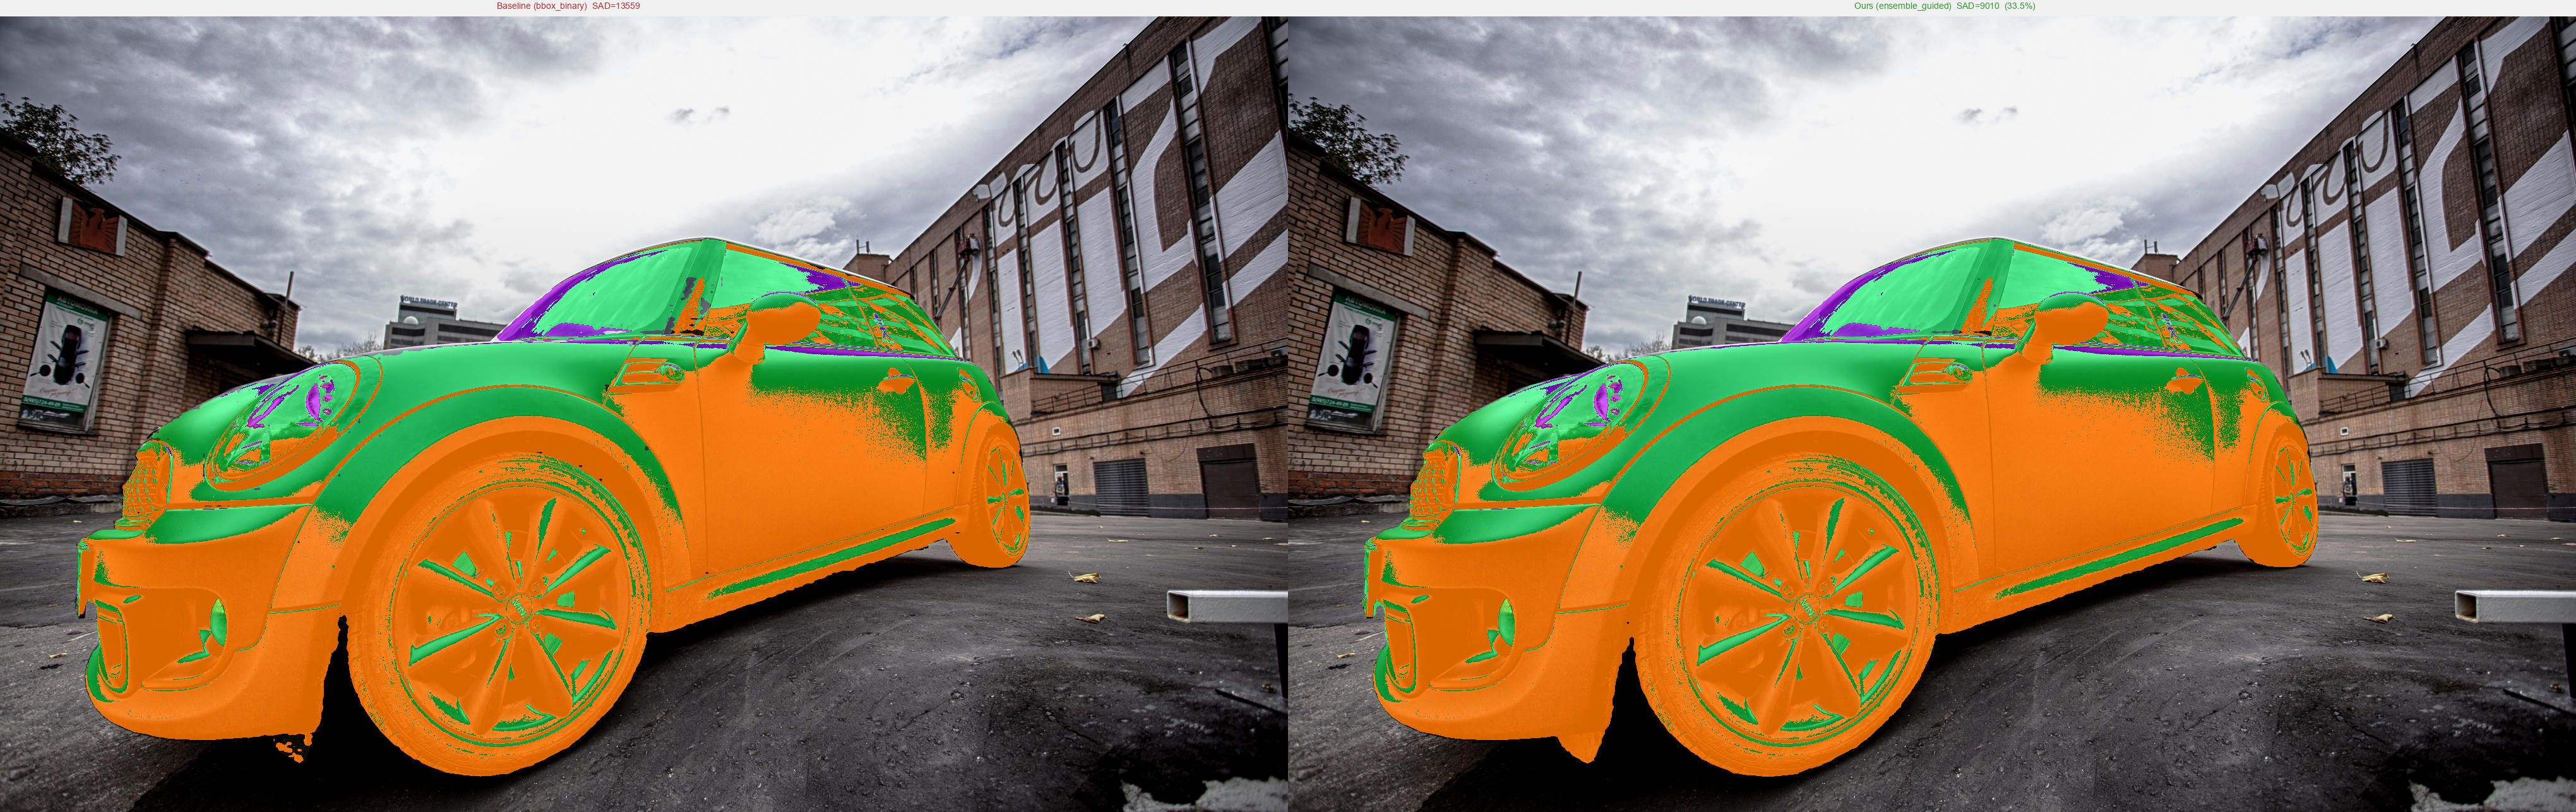
\includegraphics[width=0.92\linewidth,height=0.60\textheight,keepaspectratio]{pic/sam2_case1_compare.png}}

  \vspace{0.12em}
  \begin{columns}[T,onlytextwidth]
    \column{0.50\textwidth}
      \tcard{deepred}{1.10cm}{Baseline 问题}{%
        \small SAD=13559。车轮和车窗边缘有明显的 mask 溢出，导致前景区域偏大。}
    \column{0.50\textwidth}
      \tcard{softgreen}{1.10cm}{优化后改善}{%
        \small SAD=9010（$\downarrow$33.5\%）。边界更贴合车身轮廓，车窗和轮毂区域 mask 精度提升。}
  \end{columns}
\end{frame}

% ==================== 第 7 页：可视化案例二 ====================
\begin{frame}[t]{7. 可视化案例二：小型目标}
  \footnotesize
  \linespread{0.92}\selectfont

  \vspace{-0.2em}
  \centering
  \fcolorbox{black!25}{white}{%
    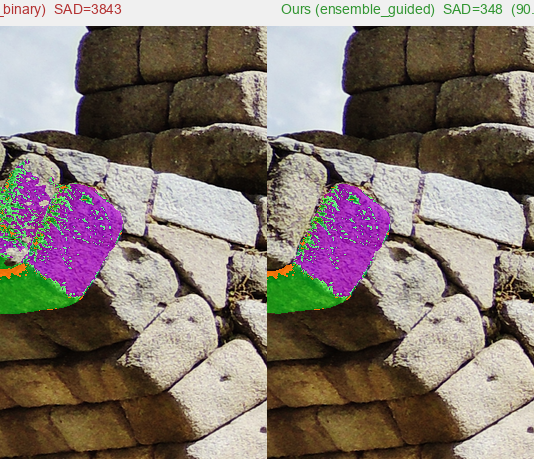
\includegraphics[width=0.80\linewidth,height=0.60\textheight,keepaspectratio]{pic/sam2_case2_compare.png}}

  \vspace{0.12em}
  \begin{columns}[T,onlytextwidth]
    \column{0.50\textwidth}
      \tcard{deepred}{1.10cm}{Baseline 问题}{%
        \small SAD=3843。微小目标（bbox 仅 117$\times$133）容易误选背景区域，mask 几乎全错。}
    \column{0.50\textwidth}
      \tcard{softgreen}{1.10cm}{优化后改善}{%
        \small SAD=348（$\downarrow$90.9\%）。Ensemble 重排序有效纠正了候选选择错误，精确捕获目标。}
  \end{columns}
\end{frame}

% ==================== 第 8 页：可视化案例三 ====================
\begin{frame}[t]{8. 可视化案例三：细结构物体}
  \footnotesize
  \linespread{0.92}\selectfont

  \vspace{-0.2em}
  \centering
  \fcolorbox{black!25}{white}{%
    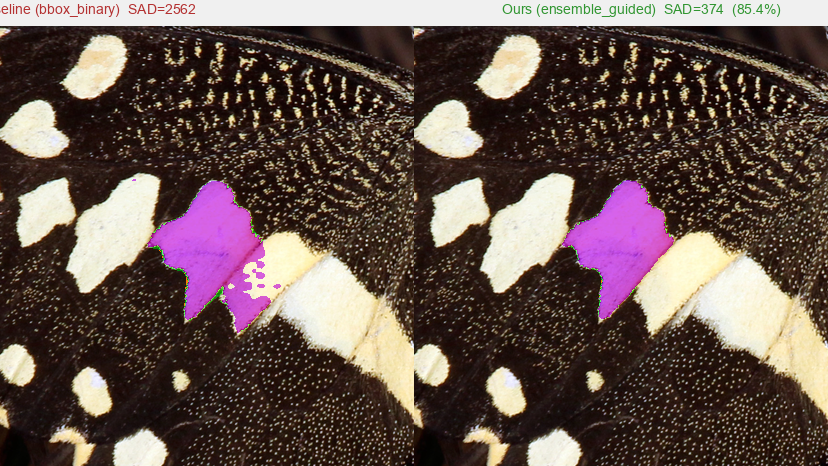
\includegraphics[width=0.80\linewidth,height=0.60\textheight,keepaspectratio]{pic/sam2_case3_compare.png}}

  \vspace{0.12em}
  \begin{columns}[T,onlytextwidth]
    \column{0.50\textwidth}
      \tcard{deepred}{1.10cm}{Baseline 问题}{%
        \small SAD=2562。细结构处有 mask 碎片和空洞，边界不完整。}
    \column{0.50\textwidth}
      \tcard{softgreen}{1.10cm}{优化后改善}{%
        \small SAD=374（$\downarrow$85.4\%）。Mask 更完整，碎片显著减少，细边缘更清晰。}
  \end{columns}
\end{frame}

% ---- 本节结束 ----


\section{精细抠图与实验}
\begin{frame}[t]{5. 从粗分割到精细 Alpha}
  \footnotesize
  \linespread{0.93}\selectfont
  \begin{columns}[T,onlytextwidth]
    \column{0.32\textwidth}
      \tcard{softgray}{2.55cm}{1. 上游定位}{%
        SAM2 / SAM3~{\scriptsize[1,\,2]} 更擅长回答“目标在哪里”，输出接近二值 mask：
        \[ M(x)\in\{0,1\}. \]
        边界处容易硬切，难以直接用于换背景。}
    \column{0.34\textwidth}
      \tcard{softorange}{2.55cm}{2. 统一 prompt}{%
        把粗定位转成 bbox / points，让后端 matting 共用同一套输入接口：
        \[ b=[x_1,y_1,x_2,y_2]. \]
        该步骤只界定空间范围，不生成最终 alpha。}
    \column{0.34\textwidth}
      \tcard{nankai}{2.55cm}{3. 精细 matting}{%
        ZIM 输出连续透明度：
        \[ \alpha(x)\in[0,1],\quad C=\alpha F+(1-\alpha)B. \]
        alpha 才能刻画毛边、透明与半透明边界。}
  \end{columns}

  \vspace{0.5em}
  \centering
  \resizebox{0.96\linewidth}{!}{%
  \begin{tikzpicture}[
    >={Latex[length=3mm,width=2.4mm]},
    node distance=7mm,
    every node/.style={font=\footnotesize},
    pcard/.style={softcardsh, rounded corners=3pt, line width=1pt, align=center, inner sep=5pt,
                  minimum width=2.45cm, minimum height=1.0cm},
    pgray/.style={pcard, draw=softgray!70!black, fill=softgray!10},
    porange/.style={pcard, draw=softorange!85!black, fill=softorange!16},
    ppurple/.style={pcard, draw=nankai!88!black, fill=nankai!14},
    pgreen/.style={pcard, draw=softgreen!72!black, fill=softgreen!15},
    pblue/.style={pcard, draw=accentblue!85!black, fill=accentblue!15},
    parrow/.style={-{Latex[length=2.8mm,width=2.3mm]}, line width=1.3pt, draw=nankai!80!black}
  ]
    \node[pgray] (sam) {\textbf{SAM2 / SAM3}\\[1pt]{\scriptsize 粗 mask}};
    \node[porange, right=of sam] (bbox) {\textbf{bbox / points}\\[1pt]{\scriptsize 标准接口}};
    \node[ppurple, right=of bbox] (zim) {\textbf{ZIM ViT-B}\\[1pt]{\scriptsize official bbox}};
    \node[pgreen, right=of zim] (ours) {\textbf{TTA-GF + BSP}\\[1pt]{\scriptsize 后端 refinement}};
    \node[pblue, right=of ours] (rgba) {\textbf{RGBA / Composer}\\[1pt]{\scriptsize 应用输出}};
    \draw[parrow] (sam) -- (bbox);
    \draw[parrow] (bbox) -- (zim);
    \draw[parrow] (zim) -- (ours);
    \draw[parrow] (ours) -- (rgba);
  \end{tikzpicture}}

  \vspace{0.45em}
  \notestrip{nankai}{\centering\scriptsize
  \textbf{关键转折：}SAM 系列负责\hilite{定位}，ZIM 负责从同一 bbox prompt 估计\hilite{软 alpha}；后续优化只改推理后处理，\hilite{不重新训练模型}。}
\end{frame}

\begin{frame}[t]{6. ZIM 的基本原理}
  \scriptsize
  \linespread{0.90}\selectfont
  \begin{block}{ZIM: Zero-Shot Image Matting for Anything}
    ZIM~{\scriptsize[5]} 面向零样本 matting：保留 SAM 式 \hilite{图像 + point / box prompt} 交互，但输出从二值 mask 变为连续的 \hilite{soft matte}，用于表达边缘像素中“前景占多少”。
  \end{block}

  \vspace{-0.18em}
  \centering
  \fcolorbox{black!25}{white}{%
  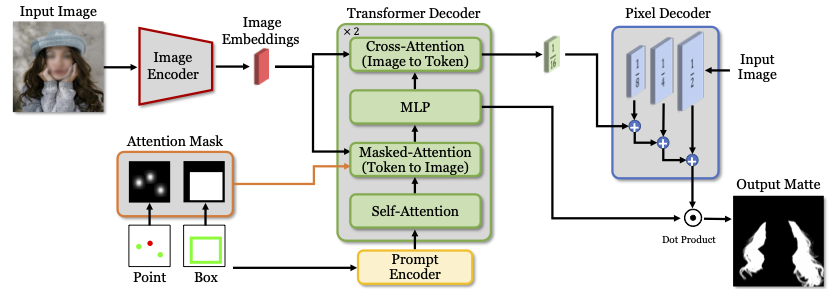
\includegraphics[width=0.98\linewidth,height=0.325\textheight,keepaspectratio]{pic/zim_method_overview.png}}

  \vspace{-0.05em}
  {\tiny Figure source: ZIM official project / Kim et al., \emph{ZIM: Zero-Shot Image Matting for Anything}, ICCV 2025.}

  \vspace{0.12em}
  \begin{columns}[T,onlytextwidth]
    \column{0.245\textwidth}
      \tcard{nankai}{1.45cm}{1. 输入图像与提示}{原图提供外观信息；点 / 框提示指定模型关注的目标位置。}
    \column{0.255\textwidth}
      \tcard{softorange}{1.45cm}{2. 提取两类特征}{图像编码器提取视觉特征；提示编码器把点 / 框转成提示特征与注意力掩码。}
    \column{0.255\textwidth}
      \tcard{softgreen}{1.45cm}{3. 提示引导解码}{解码器融合图像与提示特征，并借掩码注意力聚焦目标区域。}
    \column{0.245\textwidth}
      \tcard{accentblue}{1.45cm}{4. 输出 soft matte}{像素解码器融合多尺度特征并逐步上采样，得到连续 soft matte。}
  \end{columns}
\end{frame}

\begin{frame}[t]{7. 优化一：PromptMatte-TTA-GF}
  \footnotesize
  \linespread{0.92}\selectfont

  \notestrip{deepred}{\scriptsize
  ZIM 的单次 alpha 预测在边界处容易受到视角方向和局部纹理影响。PromptMatte-TTA-GF 将这个缺口建模为 \hilite{提示保持的等变一致性 ＋ 图像边缘投影}（Guided Filter~{\scriptsize[8]}），在不更新权重的情况下细化边界。}

  \vspace{0.04em}
  \centering
  \resizebox{\linewidth}{!}{%
  \begin{tikzpicture}[
    x=1cm, y=1cm,
    >={Latex[length=3mm,width=2.4mm]},
    every node/.style={font=\scriptsize},
    softsh/.style={blur shadow={shadow blur steps=6, shadow xshift=0.5pt,
                   shadow yshift=-0.7pt, shadow opacity=32, shadow blur radius=2pt}},
    nodebase/.style={softsh, rounded corners=3pt, line width=1pt, align=center, inner sep=5pt},
    io/.style={nodebase, draw=black!50, fill=black!5, line width=0.9pt},
    net/.style={nodebase, draw=nankai!85!black, fill=nankai!13},
    amap/.style={nodebase, draw=accentblue!82!black, fill=accentblue!14},
    flipb/.style={nodebase, draw=softorange!85!black, fill=softorange!17},
    fuse/.style={nodebase, draw=nankai!90!black, fill=nankai!18},
    gfilt/.style={nodebase, draw=softgreen!72!black, fill=softgreen!17},
    sumop/.style={softsh, circle, draw=nankai!90!black, line width=1.1pt, fill=nankai!16, inner sep=2.2pt},
    pipe/.style={-{Latex[length=2.8mm,width=2.3mm]}, line width=1.3pt, draw=nankai!80!black, rounded corners=2.5pt},
    guide/.style={-{Latex[length=2.6mm,width=2.1mm]}, line width=1.05pt,
                  draw=softgreen!62!black, dash pattern=on 3.2pt off 2.2pt},
    tab/.style={softsh, rounded corners=3pt, inner xsep=6pt, inner ysep=2.6pt, font=\tiny\bfseries}
  ]
    % ---- top branch: original prediction ----
    \node[io,   minimum width=1.78cm, minimum height=0.76cm] (orig) at (1.05,2.05) {\textbf{Original}\\$(\mathcal{I},b)$};
    \node[net,  minimum width=1.26cm, minimum height=0.76cm] (zim0) at (3.30,2.05) {\textbf{ZIM}\\$f_\theta$};
    \node[amap, minimum width=1.02cm, minimum height=0.76cm] (a0)   at (5.10,2.05) {\footnotesize$\alpha_0$};

    % ---- bottom branch: flip-equivariant prediction ----
    \node[io,    minimum width=1.78cm, minimum height=0.76cm] (flip) at (1.05,0.55) {\textbf{Flip}\\$(F(\mathcal{I}),F(b))$};
    \node[net,   minimum width=1.26cm, minimum height=0.76cm] (zim1) at (3.30,0.55) {\textbf{ZIM}\\$f_\theta$};
    \node[flipb, minimum width=1.32cm, minimum height=0.76cm] (fb)   at (5.20,0.55) {\textbf{Flip back}\\$F^{-1}$};
    \node[amap,  minimum width=1.02cm, minimum height=0.76cm] (a1)   at (7.05,0.55) {\footnotesize$\alpha_1$};

    % ---- fusion + edge-aware projection ----
    \node[sumop] (merge) at (8.35,1.30) {\footnotesize$\boldsymbol{+}$};
    \node[fuse,  minimum width=1.55cm, minimum height=0.84cm] (avg)    at (10.65,1.30) {\textbf{Average}\\$\alpha_T$};
    \node[gfilt, minimum width=1.84cm, minimum height=0.84cm] (filter) at (13.05,1.30) {\textbf{Guided Filter}\\{\tiny RGB guidance}};
    \node[amap,  minimum width=1.48cm, minimum height=0.84cm, fill=accentblue!20,
          draw=accentblue!90!black, line width=1.2pt] (out) at (15.40,1.30) {\textbf{Output}\\$\alpha_G$};

    % ---- pipeline arrows ----
    \draw[pipe] (orig) -- (zim0);
    \draw[pipe] (zim0) -- (a0);
    \draw[pipe] (flip) -- (zim1);
    \draw[pipe] (zim1) -- (fb);
    \draw[pipe] (fb)   -- (a1);
    \draw[pipe] (a0.east) -| (merge.north);
    \draw[pipe] (a1.east) -| (merge.south);
    \draw[pipe] (merge) -- (avg);
    \draw[pipe] (avg) -- (filter);
    \draw[pipe] (filter) -- (out);

    % ---- edge guidance: original RGB image guides the filter ----
    \draw[guide] (orig.north) .. controls (5.6,2.55) and (11.0,3.5) ..
      node[pos=0.55, fill=white, fill opacity=0.92, text opacity=1, rounded corners=2pt,
           inner xsep=3pt, inner ysep=1.6pt, text=softgreen!58!black, font=\tiny\bfseries] {edge guidance}
      (filter.north);

    % ---- phase grouping bands (drawn behind everything) ----
    \begin{scope}[on background layer]
      \node[fit=(orig)(flip)(a1)(merge), rounded corners=7pt,
            draw=nankai!45, line width=1pt, fill=nankai!5, inner sep=10pt] (grpA) {};
      \node[fit=(avg)(out), rounded corners=7pt,
            draw=softgreen!52!black, line width=1pt, fill=softgreen!6, inner sep=10pt] (grpB) {};
    \end{scope}

    % ---- phase tab labels sitting just above the band borders ----
    \node[tab, draw=nankai!58, fill=nankai!14, text=nankai!90!black, anchor=south west]
      at ([xshift=10pt,yshift=-1.5pt]grpA.north west) {翻转等变一致性 · Flip consistency};
    \node[tab, draw=softgreen!58!black, fill=softgreen!15, text=softgreen!52!black, anchor=south east]
      at ([xshift=-10pt,yshift=-1.5pt]grpB.north east) {边缘感知投影 · Edge-aware projection};
  \end{tikzpicture}}

  \vspace{0.12em}
  \begin{columns}[T,onlytextwidth]
    \column{0.30\textwidth}
      \ccard{accentblue}{1.04cm}{%
      {\scriptsize\textbf{\textcolor{accentblue!85!black}{Original prediction}}}\\[1pt]
      {\fontsize{7.6}{8.2}\selectfont $\alpha_0=f_\theta(\mathcal{I},b)$}\\[1pt]
      {\tiny 原图分支的 soft matte}}
    \column{0.40\textwidth}
      \ccard{nankai}{1.04cm}{%
      {\scriptsize\textbf{\textcolor{nankai!88!black}{Flip-consistent estimate}}}\\[1pt]
      {\fontsize{7.4}{8.0}\selectfont $\alpha_1=F^{-1}\!\left(f_\theta(F(\mathcal{I}),F(b))\right),\quad \alpha_T=\tfrac{\alpha_0+\alpha_1}{2}$}\\[1pt]
      {\tiny 对齐后平均，降低方向敏感误差}}
    \column{0.30\textwidth}
      \ccard{softgreen}{1.04cm}{%
      {\scriptsize\textbf{\textcolor{softgreen!60!black}{Edge-aware projection}}}\\[1pt]
      {\fontsize{7.6}{8.2}\selectfont $\alpha_G=\mathrm{GF}(\mathcal{I},\alpha_T)$}\\[1pt]
      {\tiny RGB guidance 保边平滑}}
  \end{columns}
\end{frame}

\begin{frame}[t]{8. 优化二：Box-Support Prior}
  \footnotesize
  \linespread{0.92}\selectfont

  \notestrip{nankai}{\scriptsize
  \textbf{动机：}TTA-GF 之后，少数样本仍会在 official bbox 之外出现轻微 alpha 泄漏。\hilite{Box-Support Prior（BSP）} 以检测框作为空间先验，对框外做温和抑制——一项\hilite{保守的稳定化后处理}。}

  \vspace{0.2em}
  \centering
  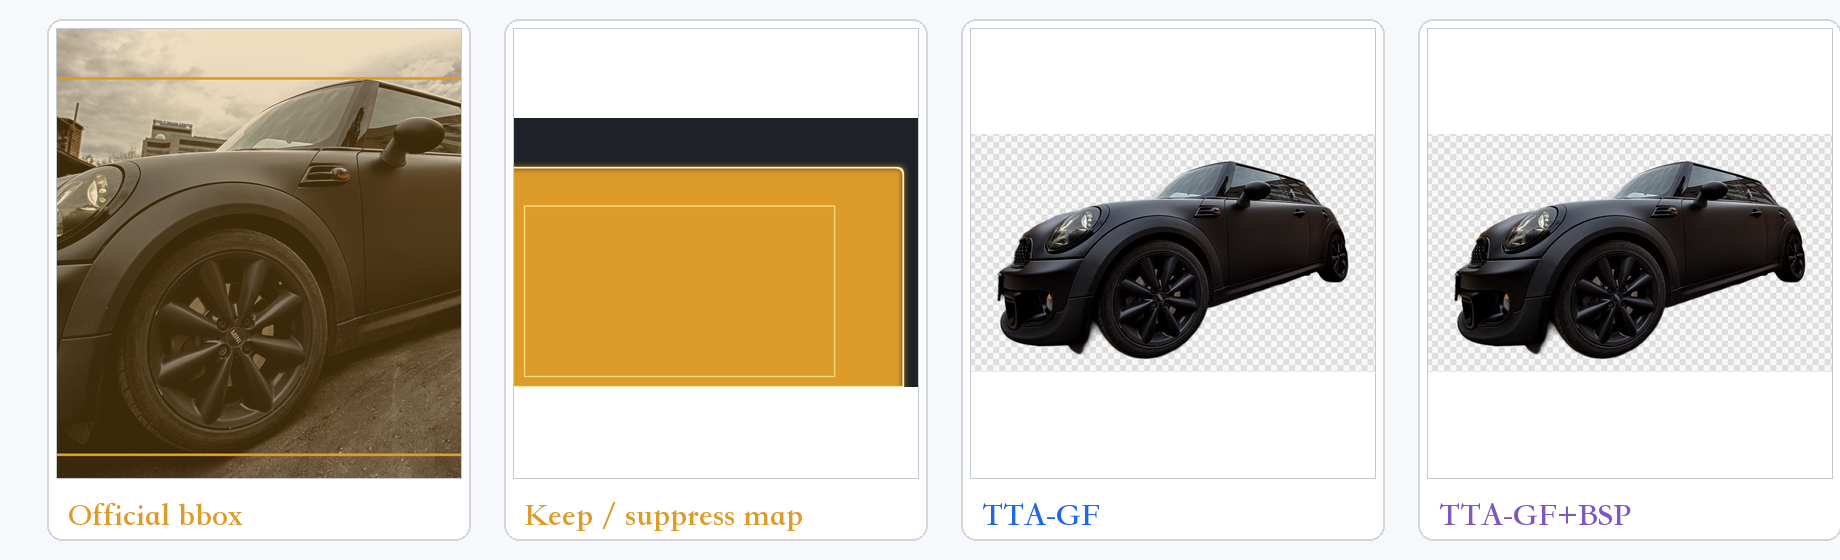
\includegraphics[width=\linewidth,height=0.345\textheight,keepaspectratio]{pic/final/slides/06_box_support_prior_cards.png}

  \vspace{0.24em}
  \begin{columns}[T,onlytextwidth]
    \column{0.34\textwidth}
      \tcard{softorange}{1.55cm}{bbox support map}{%
        official bbox 作为空间支持：框内保留、框外温和抑制。\par\vspace{2pt}%
        {\centering$G(x)=S(x)+\bigl(1-S(x)\bigr)\eta$\par}}
    \column{0.34\textwidth}
      \tcard{nankai}{1.55cm}{alpha re-weight}{%
        对 TTA-GF 输出轻量重加权，抑制框外泄漏：\par\vspace{2pt}%
        {\centering$\alpha_B(x)=\alpha_G(x)\bigl(1-\lambda+\lambda G(x)\bigr)$\par}}
    \column{0.32\textwidth}
      \tcard{softgreen}{1.55cm}{稳定化效果}{%
        框外泄漏被进一步抑制、主体边界更稳定；作为 TTA-GF 之上的轻量补充，整体更稳健。}
  \end{columns}
\end{frame}

\begin{frame}[t]{9. valid706 主表结果}
  \footnotesize
  \linespread{0.92}\selectfont
  \begin{columns}[T,onlytextwidth]
    \column{0.5\textwidth}
      \notestrip{softgray}{\scriptsize
      \textbf{数据集 · valid706：}取自 MicroMat 验证集中带 \emph{official text prompt} 的 \textbf{706} 张图像子集；每张都配有官方 bbox / points 提示与高质量 GT alpha，便于在\hilite{统一提示输入}下做公平、可复现的对比。}
    \column{0.5\textwidth}
      \notestrip{softgray}{\scriptsize
      \textbf{评测方法：}baseline 与各优化方法均使用\hilite{同一 official bbox}推理，再用同一脚本统一评分（Composer demo 不计入）；四项指标均\hilite{越低越好}（$\downarrow$）。}
  \end{columns}

  \vspace{0.04em}
  {\centering
  \scriptsize
  \setlength{\tabcolsep}{3.5pt}
  \renewcommand{\arraystretch}{1.0}
  \resizebox{0.97\linewidth}{!}{%
  \begin{tabular}{lrrrr}
    \toprule
    Method & SAD $\downarrow$ & MSE $\downarrow$ & MAE$_{\times1000}\downarrow$ & Boundary SAD $\downarrow$ \\
    \midrule
    ZIM bbox baseline & 2.320107 & 0.000579536 & 0.825480 & 0.736623 \\
    PromptMatte-TTA-GF & 2.123826 & 0.000445816 & 0.753268 & 0.638556 \\
    \textbf{PromptMatte-TTA-GF+BSP} & \textbf{2.122658} & \textbf{0.000445414} & \textbf{0.752814} & \textbf{0.638283} \\
    \bottomrule
  \end{tabular}}\par}

  \vspace{0.5em}
  \begin{columns}[T,onlytextwidth]
    \column{0.24\textwidth}
      \metricchip{softgreen}{SAD\,$\downarrow$\\{\tiny 绝对误差和}}{$-8.51\%$}
    \column{0.24\textwidth}
      \metricchip{softgreen}{MSE\,$\downarrow$\\{\tiny 均方误差}}{$-23.14\%$}
    \column{0.24\textwidth}
      \metricchip{softgreen}{MAE$_{\times1000}$\,$\downarrow$\\{\tiny 平均绝对误差}}{$-8.80\%$}
    \column{0.28\textwidth}
      \metricchip{nankai}{Boundary SAD\,$\downarrow$\\{\tiny 边界带误差}}{$-13.35\%$}
  \end{columns}

  \vspace{0.06em}
  \notestrip{nankai}{\scriptsize
  \textbf{结论：}我们的方法（PromptMatte-TTA-GF\,+\,BSP）在 SAD、MSE、MAE、Boundary SAD \hilite{四项指标上全面优于 ZIM bbox baseline}。}
\end{frame}

\begin{frame}[t,label=vis-car]{10. 可视化案例一：整车目标}
  \footnotesize
  \linespread{0.92}\selectfont
  \centering
  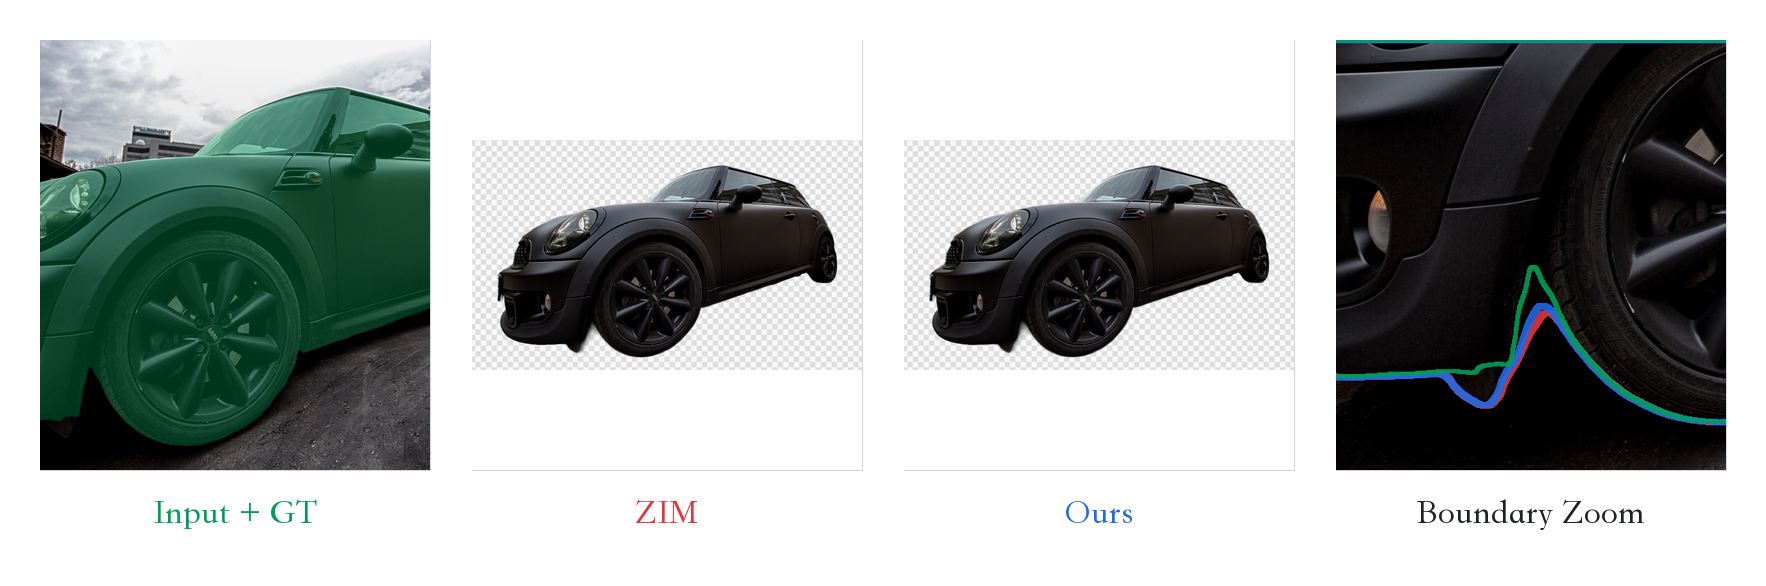
\includegraphics[width=0.98\linewidth,height=0.55\textheight,keepaspectratio]{pic/final/clean/01_0100_1_clean_comparison.png}

  \vspace{0.36em}
  \mpill[nankai]{Boundary SAD}{$-13.35\%$}\quad\mpill[softgray]{SAD}{$-8.51\%$}\quad\mpill[softgray]{MSE}{$-23.14\%$}\quad\mpill[softgray]{MAE$_{\times1000}$}{$-8.80\%$}

  \vspace{0.38em}
  \notestrip{nankai}{\scriptsize
  车轮弧线和车身外沿是这一例最明显的差异：ZIM 的红色轮廓在轮胎附近有局部外扩，和 GT 绿线存在偏移；我们的蓝色轮廓更贴近车轮外轮廓，车身硬边的外溢也更少。}
\end{frame}

\begin{frame}[t,label=vis-device]{11. 可视化案例二：设备部件}
  \footnotesize
  \linespread{0.92}\selectfont
  \centering
  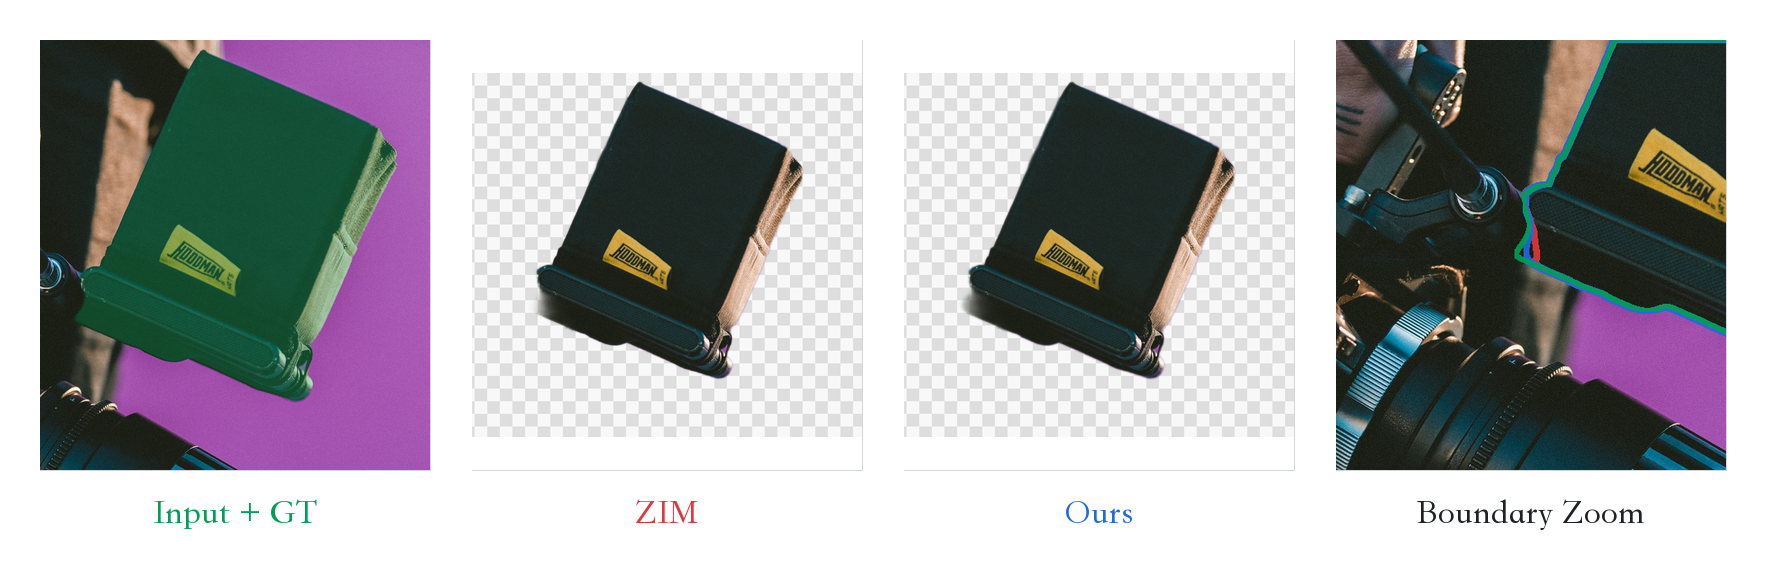
\includegraphics[width=0.98\linewidth,height=0.55\textheight,keepaspectratio]{pic/final/clean/02_0067_2_clean_comparison.png}

  \vspace{0.36em}
  \mpill[nankai]{MSE}{$-23.14\%$}\quad\mpill[softgray]{Boundary SAD}{$-13.35\%$}\quad\mpill[softgray]{SAD}{$-8.51\%$}\quad\mpill[softgray]{MAE$_{\times1000}$}{$-8.80\%$}

  \vspace{0.38em}
  \notestrip{nankai}{\scriptsize
  设备斜边和下方支架区域更容易暴露边界问题：ZIM 在边缘处有轻微毛刺和背景残留；我们的结果沿斜边更平直，支架附近更干净，主体轮廓也更完整。}
\end{frame}

\begin{frame}[t,label=vis-balloon]{12. 可视化案例三：热气球}
  \footnotesize
  \linespread{0.92}\selectfont
  \centering
  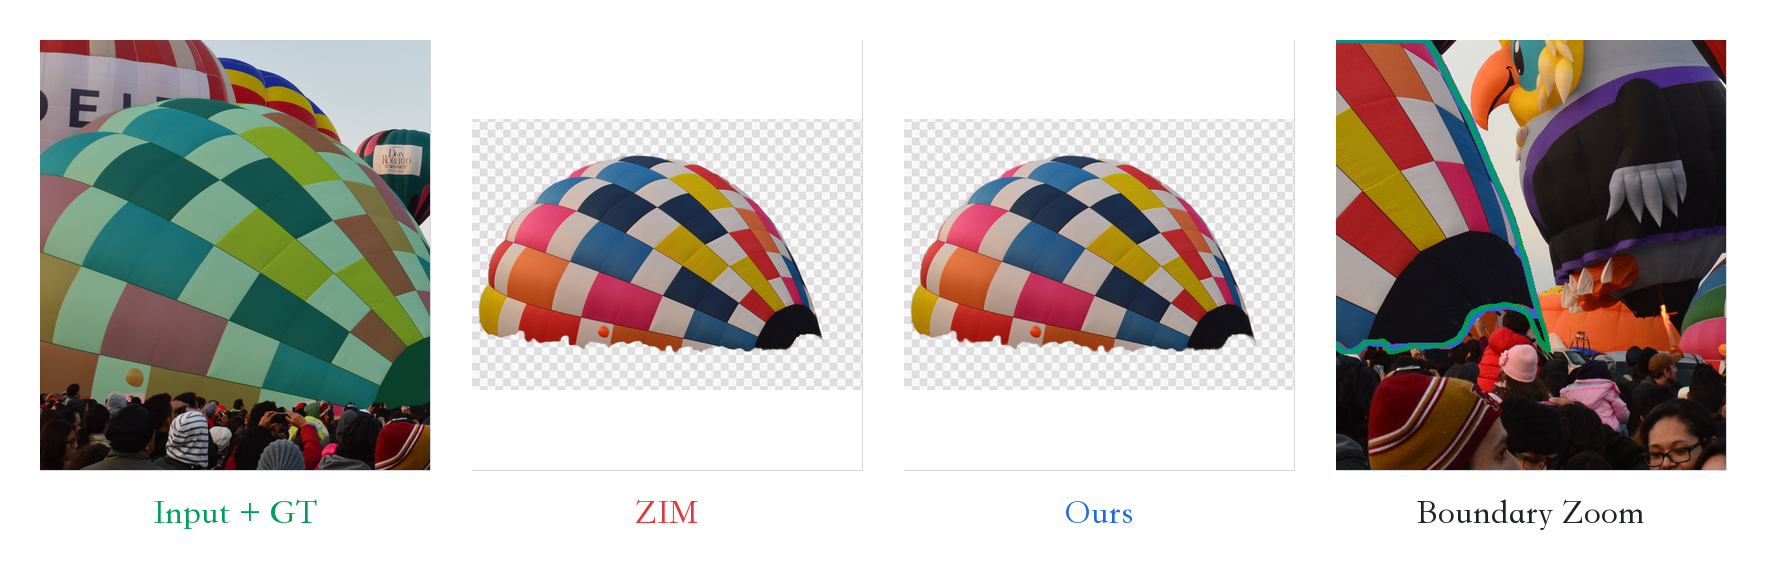
\includegraphics[width=0.98\linewidth,height=0.55\textheight,keepaspectratio]{pic/final/clean/03_0085_0_clean_comparison.png}

  \vspace{0.36em}
  \mpill[nankai]{SAD}{$-8.51\%$}\quad\mpill[softgray]{MAE$_{\times1000}$}{$-8.80\%$}\quad\mpill[softgray]{MSE}{$-23.14\%$}\quad\mpill[softgray]{Boundary SAD}{$-13.35\%$}

  \vspace{0.38em}
  \notestrip{nankai}{\scriptsize
  热气球的弧形边界和彩色拼接纹理对抠图很敏感。ZIM 在局部弧线处会出现偏移，容易吞掉前景或带入人群背景；我们的蓝色边界更接近 GT，气球布边缘更连续、更稳定。}
\end{frame}

\begin{frame}[t]{13. RGBA / Composer 是什么}
  \footnotesize
  \linespread{0.92}\selectfont
  \begin{block}{从 alpha 到透明前景}
    把前面优化得到的 \hilite{软 alpha} 变成可编辑的透明前景，再接到换背景和背景虚化流程中，检查最终合成边缘是否干净。
  \end{block}

  \vspace{-0.12em}
  \begin{columns}[T,onlytextwidth]
    \column{0.57\textwidth}
      \centering
      \begin{tikzpicture}[
        >={Latex[length=2.8mm,width=2.3mm]},
        node distance=3mm,
        every node/.style={font=\scriptsize},
        vcard/.style={softcardsh, rounded corners=3pt, line width=1pt, align=center, inner sep=3pt,
                      minimum width=4.4cm, minimum height=0.7cm},
        vblue/.style={vcard, draw=accentblue!82!black, fill=accentblue!13},
        vpurple/.style={vcard, draw=nankai!88!black, fill=nankai!13},
        vgreen/.style={vcard, draw=softgreen!72!black, fill=softgreen!15},
        varrow/.style={-{Latex[length=2.8mm,width=2.3mm]}, line width=1.3pt, draw=nankai!80!black}
      ]
        \node[vblue] (alpha) {\textbf{1. Soft Alpha}\\[1pt]{\scriptsize 每个像素的前景透明度 $\alpha(x)$}};
        \node[vpurple, below=of alpha] (rgba) {\textbf{2. RGBA Foreground}\\[1pt]{\scriptsize 主体颜色 $F$ ＋ 透明通道 $\alpha$}};
        \node[vgreen, below=of rgba] (out) {\textbf{3. Composer Output}\\[1pt]{\scriptsize 透明 PNG / Replace BG / Blur BG}};
        \draw[varrow] (alpha) -- (rgba);
        \draw[varrow] (rgba) -- (out);
      \end{tikzpicture}

      \vspace{0.08em}
      \ccard{nankai}{0.98cm}{\scriptsize
      $\mathrm{RGBA}(x)=\bigl(F_R(x),F_G(x),F_B(x),\alpha(x)\bigr)$\\[2pt]
      $C(x)=\alpha(x)F(x)+\bigl(1-\alpha(x)\bigr)B(x)$}

    \column{0.41\textwidth}
      \begin{block}{关键概念}
        \textbf{前景 $F$：}要保留的主体颜色，来自原图。\\
        \textbf{Alpha：}透明度，不是硬二值 mask。\\
        \textbf{RGBA：}RGB 存颜色，A 存透明度。
      \end{block}

      \vspace{-0.1em}
      \begin{block}{Composer 输出与边界检查}
        Composer 使用优化后的 alpha 完成透明 PNG、换背景和背景虚化。合成结果会放大边界问题：白边、黑边、漏洞或残影都会直接暴露；该模块不重新预测目标，也不参与 valid706。
      \end{block}
  \end{columns}
\end{frame}

\begin{frame}[t]{14. RGBA / Composer 案例一}
  \small
  \linespread{0.94}\selectfont
  \centering
  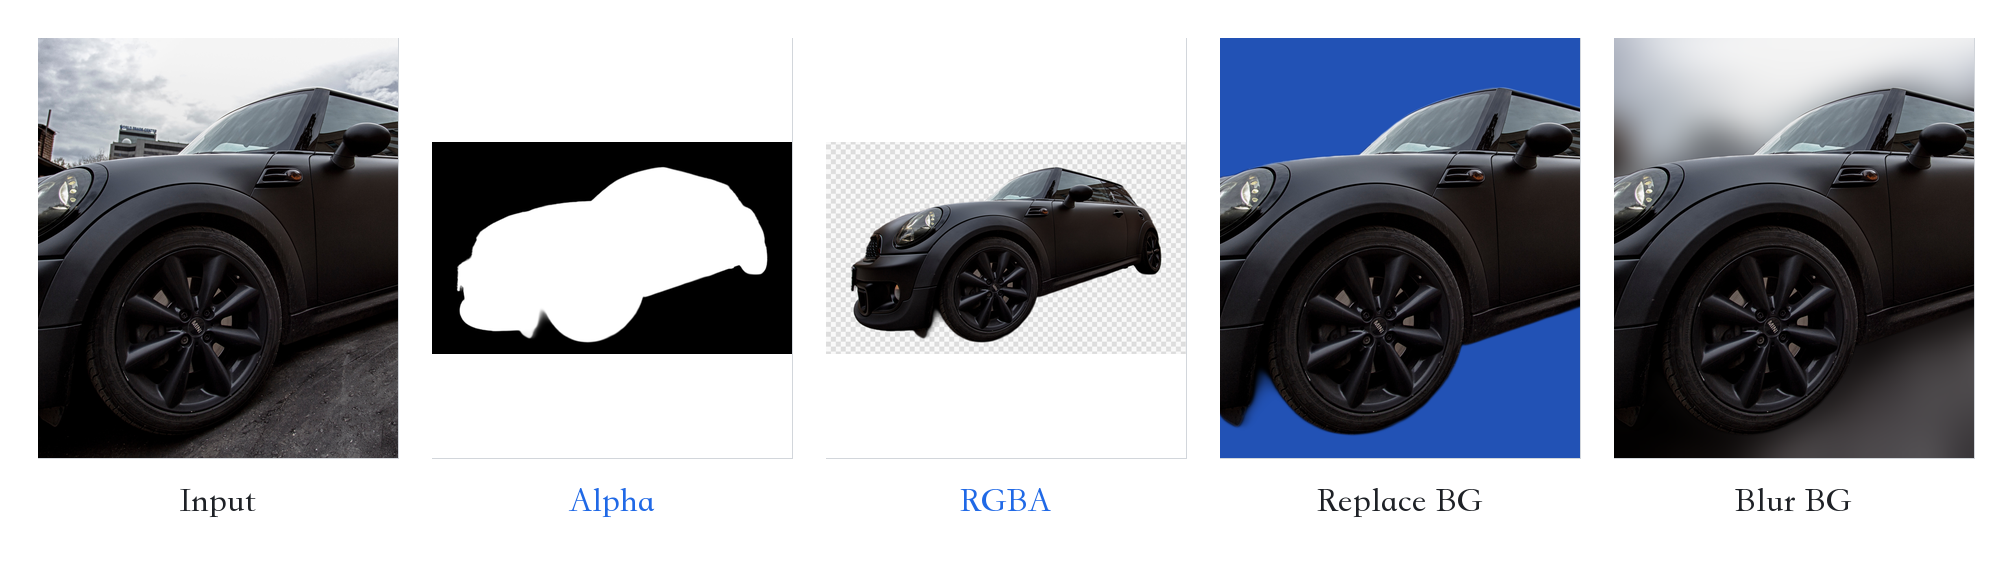
\includegraphics[width=0.98\linewidth,height=0.53\textheight,keepaspectratio]{pic/final/clean/04_0100_1_clean_alpha_composer.png}

  \vspace{0.3em}
  \notestrip{nankai}{\scriptsize
  \hilite{alpha 即 RGBA 的透明通道}，通过 alpha blending 即可完成\hilite{换背景}与\hilite{背景虚化}。图中车轮和车身边缘在两种合成结果中仍\hilite{保持贴合}，没有明显白边、黑边或缺口，说明边界优化不仅改善指标，也\hilite{提升了最终编辑效果}。}
\end{frame}

\begin{frame}[t]{15. RGBA / Composer 案例二}
  \small
  \linespread{0.94}\selectfont
  \centering
  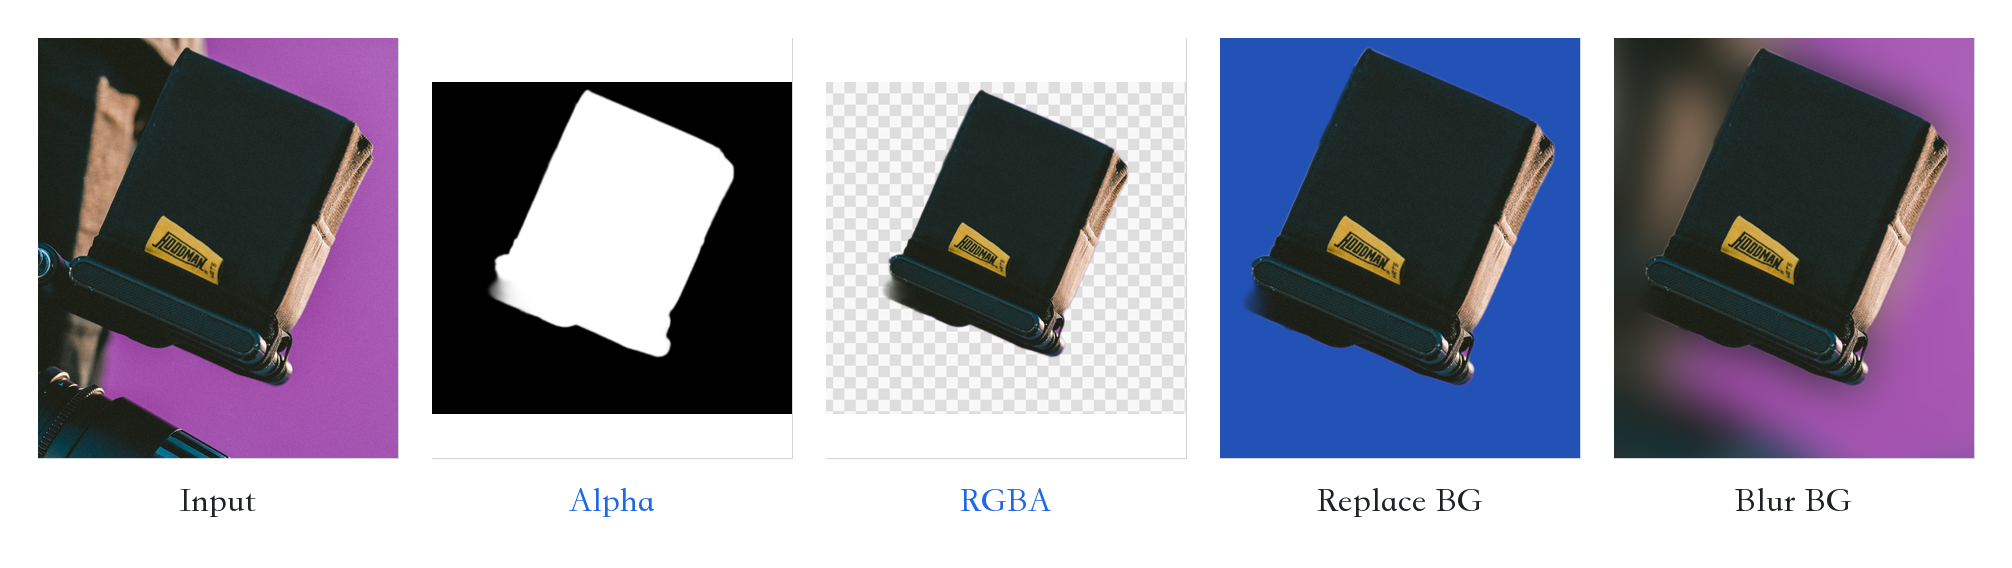
\includegraphics[width=0.98\linewidth,height=0.53\textheight,keepaspectratio]{pic/final/clean/05_0067_2_clean_alpha_composer.png}

  \vspace{0.3em}
  \notestrip{nankai}{\scriptsize
  \hilite{设备斜边与下方支架}是最容易暴露 alpha 不稳定的区域；边界偏移会在换背景后表现为毛边、残影或背景漏入。图中 \hilite{RGBA 前景、蓝底替换、虚化背景} 的轮廓基本一致，说明优化后的 alpha 能\hilite{稳定接入后续编辑流程}。}
\end{frame}

% ===== 队友占位章节：视频 matting 与应用（张竣翔）=====
% !TeX program = xelatex
% ============================================================================
%  队友章节：视频 matting 与应用   ——   负责人：张竣翔
% ----------------------------------------------------------------------------
%  · 本文件由主文件 slides.tex 通过 % !TeX program = xelatex
% ============================================================================
%  队友章节：视频 matting 与应用   ——   负责人：张竣翔
% ----------------------------------------------------------------------------
%  · 本文件由主文件 slides.tex 通过 % !TeX program = xelatex
% ============================================================================
%  队友章节：视频 matting 与应用   ——   负责人：张竣翔
% ----------------------------------------------------------------------------
%  · 本文件由主文件 slides.tex 通过 \input{sections/video.tex} 引入，
%    继承主文件导言区的全部宏 / 配色 / 字体，无需自带 \documentclass 或 \begin{document}。
%  · 直接在下面增删 \begin{frame}[t]{标题} ... \end{frame} 即可。
%  · 可复用样式：
%       \hilite{} \tcard{} \ccard{} \notestrip{} \metricchip{} \mpill[] \pill[]
%     可选 accent：nankai、accentblue、softgreen、softorange、softgray、deepred
% ============================================================================

\section{视频与应用}

\begin{frame}[t]{视频抠图与时序平滑}
  \scriptsize
  \linespread{0.98}\selectfont
  
  \begin{columns}[T,onlytextwidth]
    \column{0.48\textwidth}
      \begin{block}{问题：视频 alpha 抖动}
        \begin{itemize}
          \setlength{\itemsep}{0.2em}
          \item MatAnyone2~{\scriptsize[7]} 逐帧推理时，alpha 存在帧间\hilite{抖动与边界闪烁}；
          \item 直接替换背景会放大这些不稳定，导致视觉不自然；
          \item 需要一种\hilite{保持细节}的时序平滑策略。
        \end{itemize}
      \end{block}
      
      \vspace{0.2em}
      \begin{block}{解决方案：边界带时序平滑}
        \centering
        \resizebox{0.95\linewidth}{!}{%
        \begin{tikzpicture}[
          >={Latex[length=2.5mm,width=2mm]},
          node distance=3mm,
          every node/.style={font=\scriptsize},
          vcard/.style={rounded corners=2pt, line width=0.8pt, align=center, inner sep=3pt},
          vblue/.style={vcard, draw=accentblue!82!black, fill=accentblue!12},
          vpurple/.style={vcard, draw=nankai!88!black, fill=nankai!12},
          vgreen/.style={vcard, draw=softgreen!72!black, fill=softgreen!14},
          varrow/.style={-{Latex[length=2.5mm,width=2mm]}, line width=1.2pt, draw=nankai!80!black}
        ]
          \node[vblue] (input) {\textbf{输入}\\alpha video};
          \node[vpurple, right=of input] (detect) {\textbf{边界检测}\\$0.05<\alpha<0.95$};
          \node[vgreen, right=of detect] (smooth) {\textbf{时序平滑}\\EMA / Bidirectional};
          \node[vblue, right=of smooth] (output) {\textbf{输出}\\稳定 alpha};
          \draw[varrow] (input) -- (detect);
          \draw[varrow] (detect) -- (smooth);
          \draw[varrow] (smooth) -- (output);
        \end{tikzpicture}}
        
        \vspace{0.2em}
        \scriptsize
        仅在边界区域（$\alpha\in[0.05,0.95]$）施加平滑，\hilite{保护前景核区与背景}，避免过度模糊。
      \end{block}
      
    \column{0.48\textwidth}
      \begin{block}{7 种平滑策略对比}
        \centering
        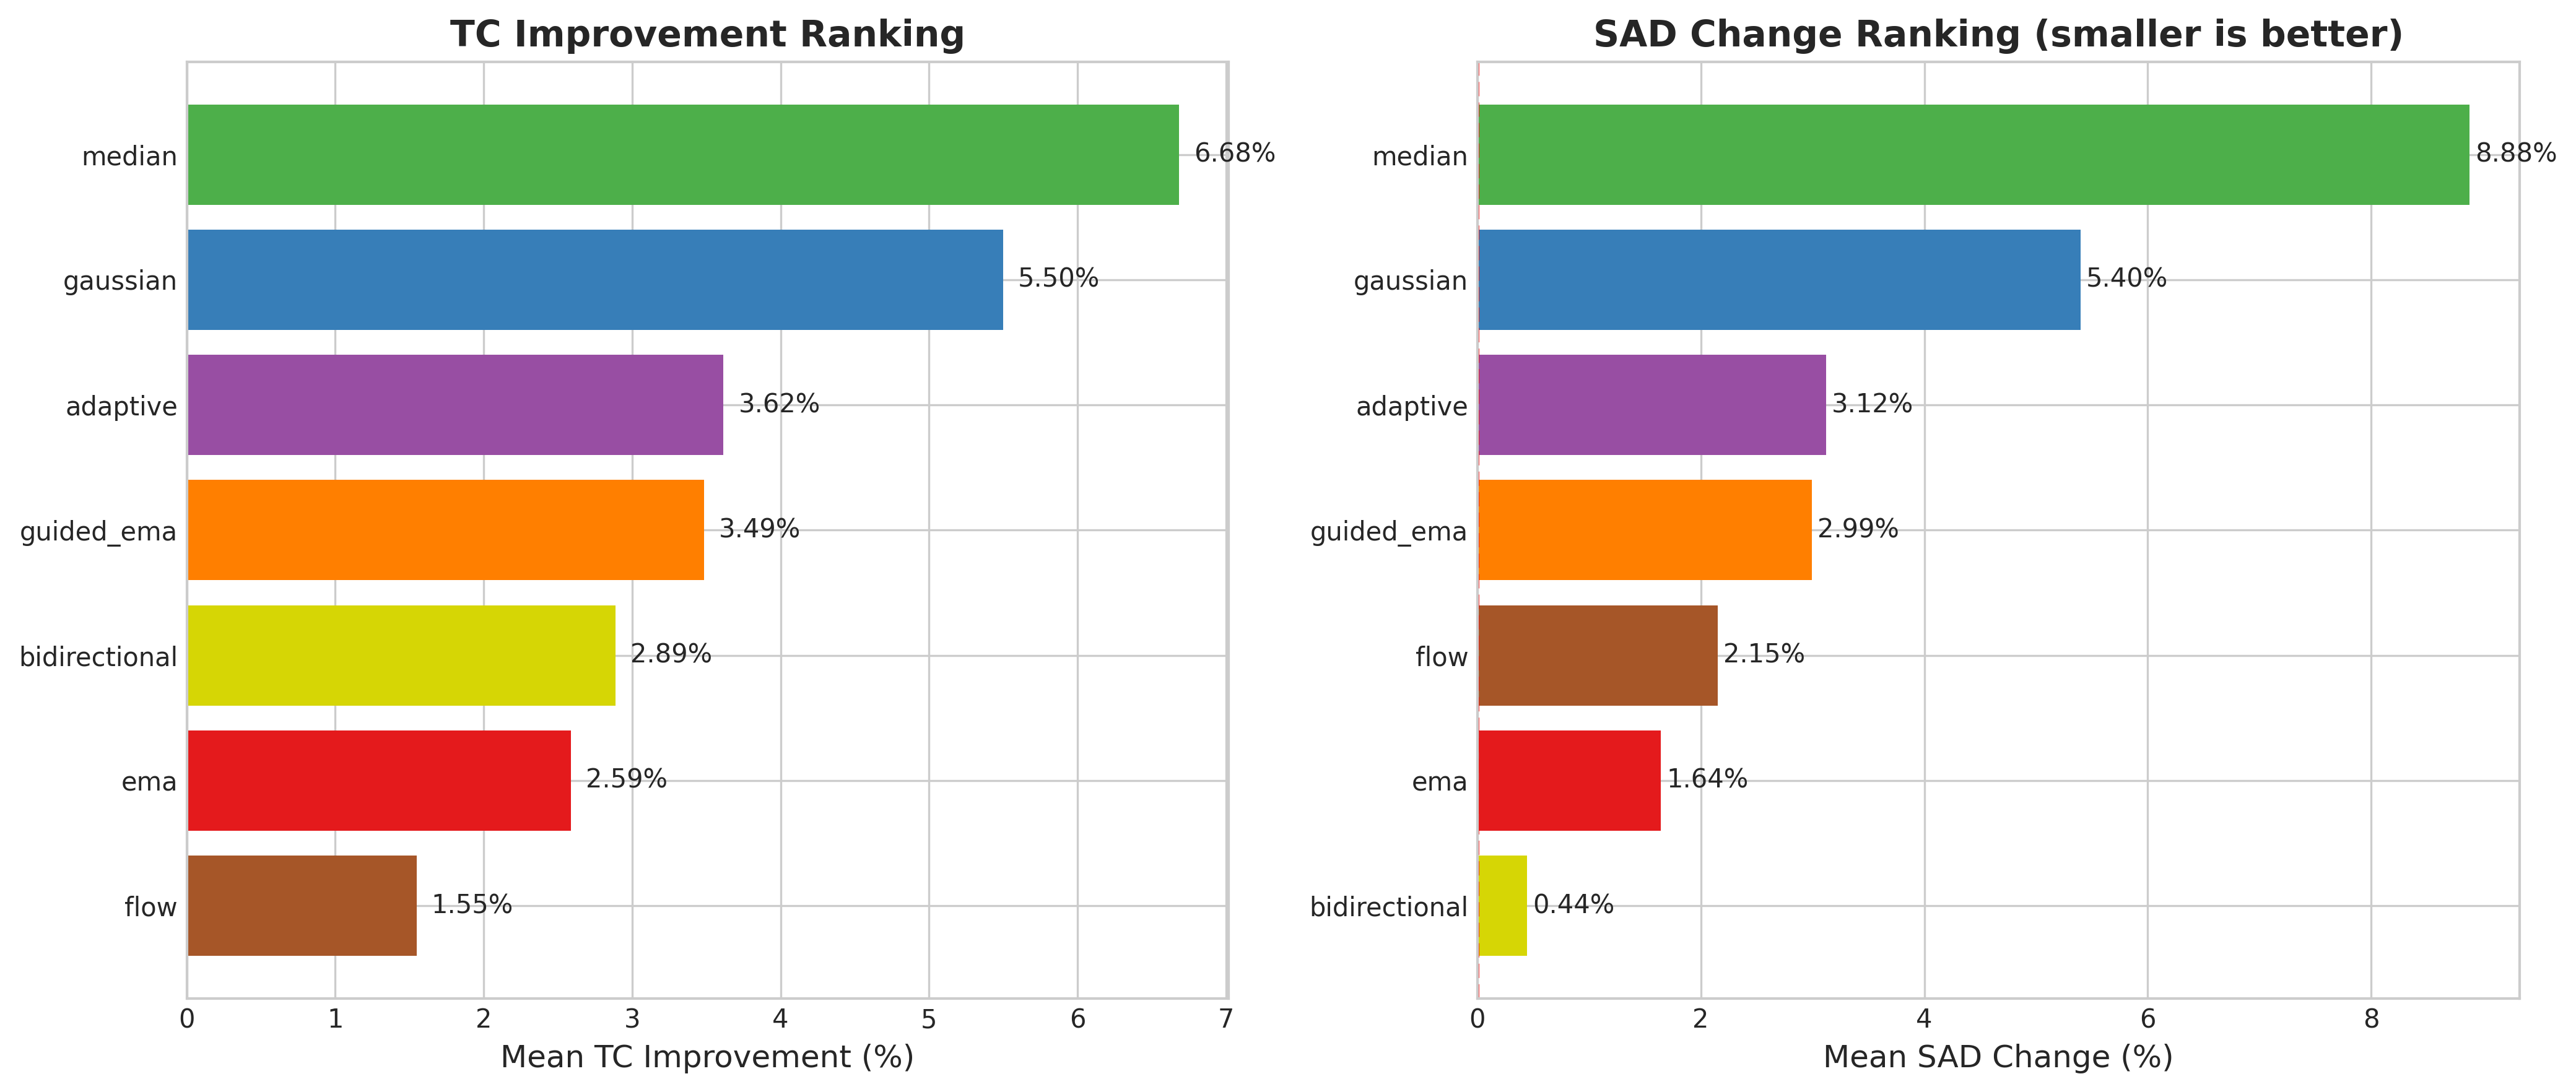
\includegraphics[width=0.95\linewidth]{pic/figure6_performance_ranking.png}
        \vspace{0.1em}
        {\scriptsize TC 提升排名（左）与 SAD 变化排名（右）}
      \end{block}
  \end{columns}
\end{frame}

\begin{frame}[t]{7 种平滑策略性能评估}
  \scriptsize
  \linespread{0.50}\selectfont
  
  \begin{block}{实验设置}
    \scriptsize
    \begin{itemize}
      \setlength{\itemsep}{0.1em}
      \item \textbf{数据集：}YouTubeMatte (10 视频) + VideoMatt (10 视频)，共 20 个测试视频；
      \item \textbf{评估指标：}TC（时序一致性）、SAD（绝对误差和）、MSE、Gradient；
      \item \textbf{方法：}EMA、Gaussian、Median、Adaptive、Guided EMA、Bidirectional、Flow。
    \end{itemize}
  \end{block}
  
  \vspace{0.1em}
  \centering
  \resizebox{0.9\linewidth}{!}{%
  \begin{tabular}{lcccc}
    \toprule
    \textbf{方法} & \textbf{TC 提升 (\%)} & \textbf{SAD 变化 (\%)} & \textbf{MSE 变化 (\%)} & \textbf{细节保留} \\
    \midrule
    Median & 6.68 & +8.88 & +23.91 & Poor \\
    Gaussian & 5.50 & +5.40 & +11.42 & Fair \\
    Adaptive & 3.62 & +3.12 & +5.88 & Fair \\
    Guided EMA & 3.49 & +2.99 & +5.28 & Fair \\
    \textbf{Bidirectional} & \textbf{2.89} & \textbf{+0.44} & \textbf{-0.12} & \textbf{Excellent} \\
    EMA & 2.59 & +1.64 & +2.40 & Good \\
    Flow & 1.55 & +2.15 & +3.62 & Fair \\
    \bottomrule
  \end{tabular}}
  
  
  \vspace{0.1em}
  \notestrip{nankai}{\scriptsize
  \textbf{关键发现：}Bidirectional 是\hilite{唯一能同时改善 TC 和保持精度}的方法，细节保留最佳。
  }
\end{frame}

\begin{frame}[t]{方法对比散点图}
  \scriptsize
  \linespread{0.92}\selectfont
  
  \begin{columns}[T,onlytextwidth]
    \column{0.60\textwidth}
      \centering
      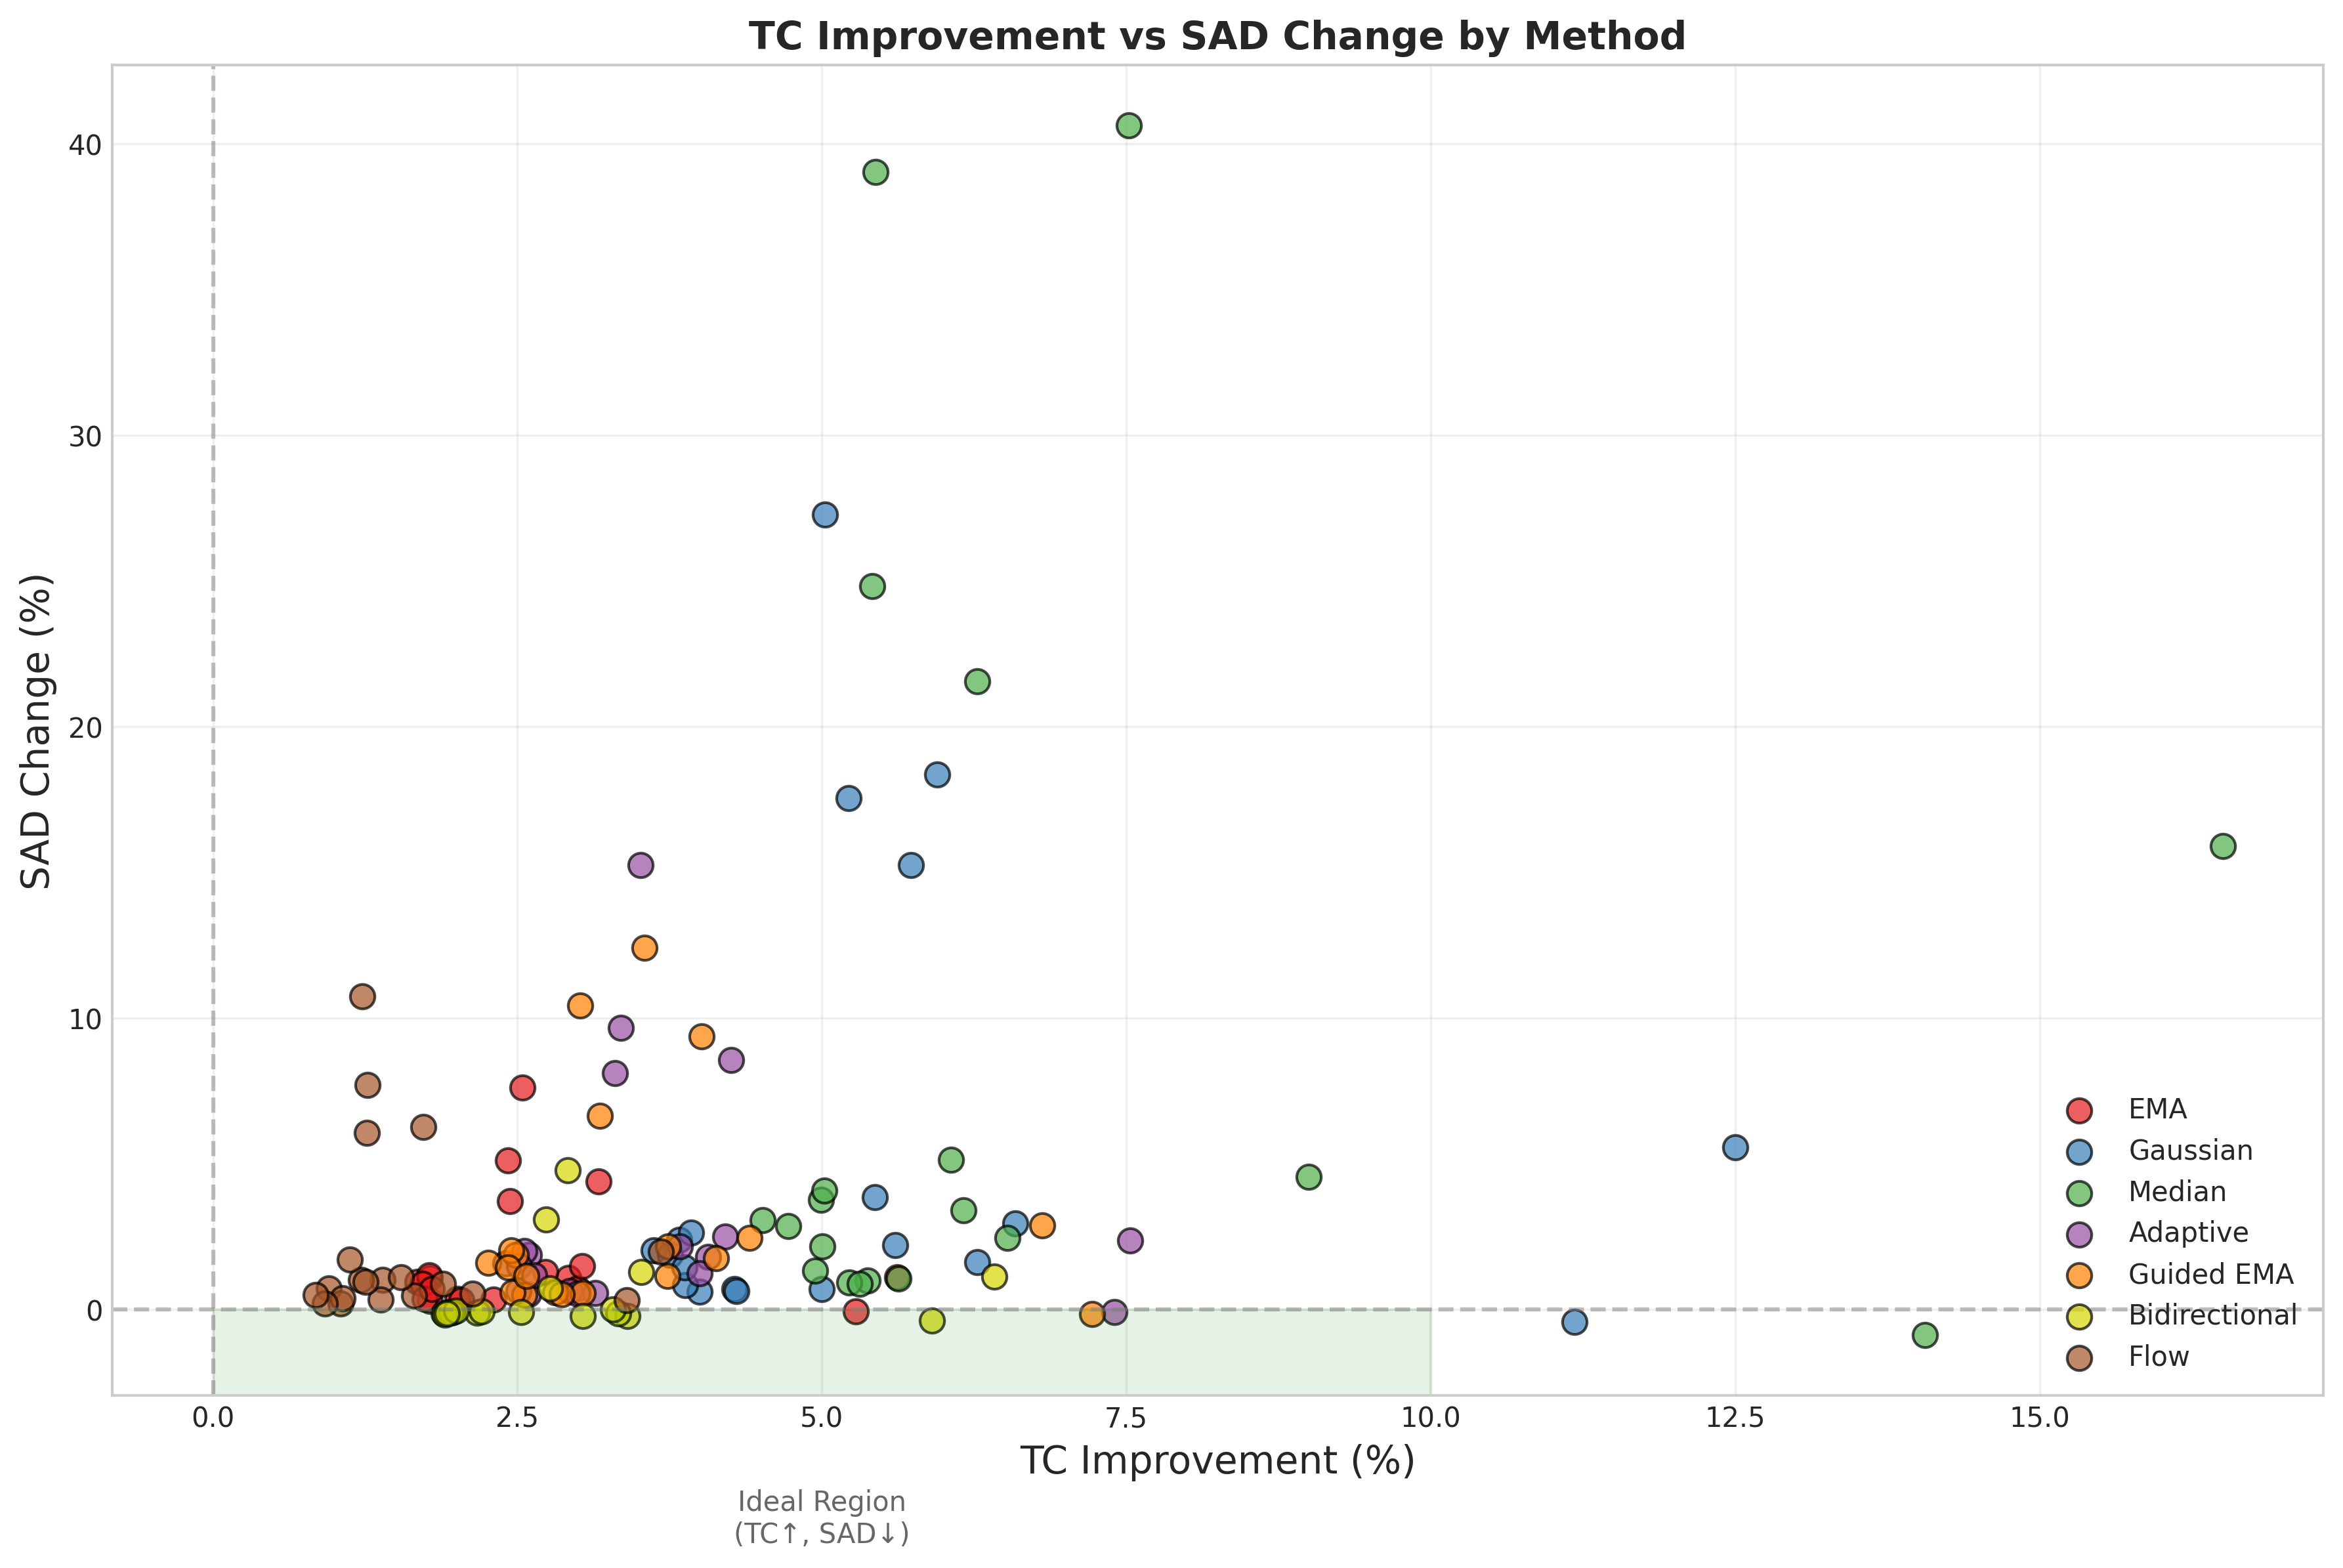
\includegraphics[width=\linewidth]{pic/figure1_tc_vs_sad_scatter.png}
      \vspace{0.1em}
      {\scriptsize  每个点代表一个视频的最佳结果}
      
    \column{0.4\textwidth}
      \begin{block}{解读}
        \begin{itemize}
          \setlength{\itemsep}{0.2em}
          \item 绿色区域：理想方向（TC↑，SAD↓）
          \item \textbf{Bidirectional}：最接近理想区域
          \item Median：TC 提升最大，但 SAD 增加显著
        \end{itemize}
      \end{block}
      
      \vspace{0.3em}
      \begin{block}{最佳参数}
        \scriptsize
        \begin{tabular}{ll}
          \toprule
          \textbf{方法} & \textbf{最佳参数} \\
          \midrule
          Median & window=7 \\
          Gaussian & sigma=2.0, window=7 \\
          \textbf{Bidirectional} & \textbf{alpha=0.7} \\
          \bottomrule
        \end{tabular}
      \end{block}
  \end{columns}
\end{frame}

\begin{frame}[t]{各方法性能分布箱线图}
  \scriptsize
  \linespread{0.98}\selectfont
  
  \begin{columns}[T,onlytextwidth]
    \column{0.7\textwidth}
      \centering
      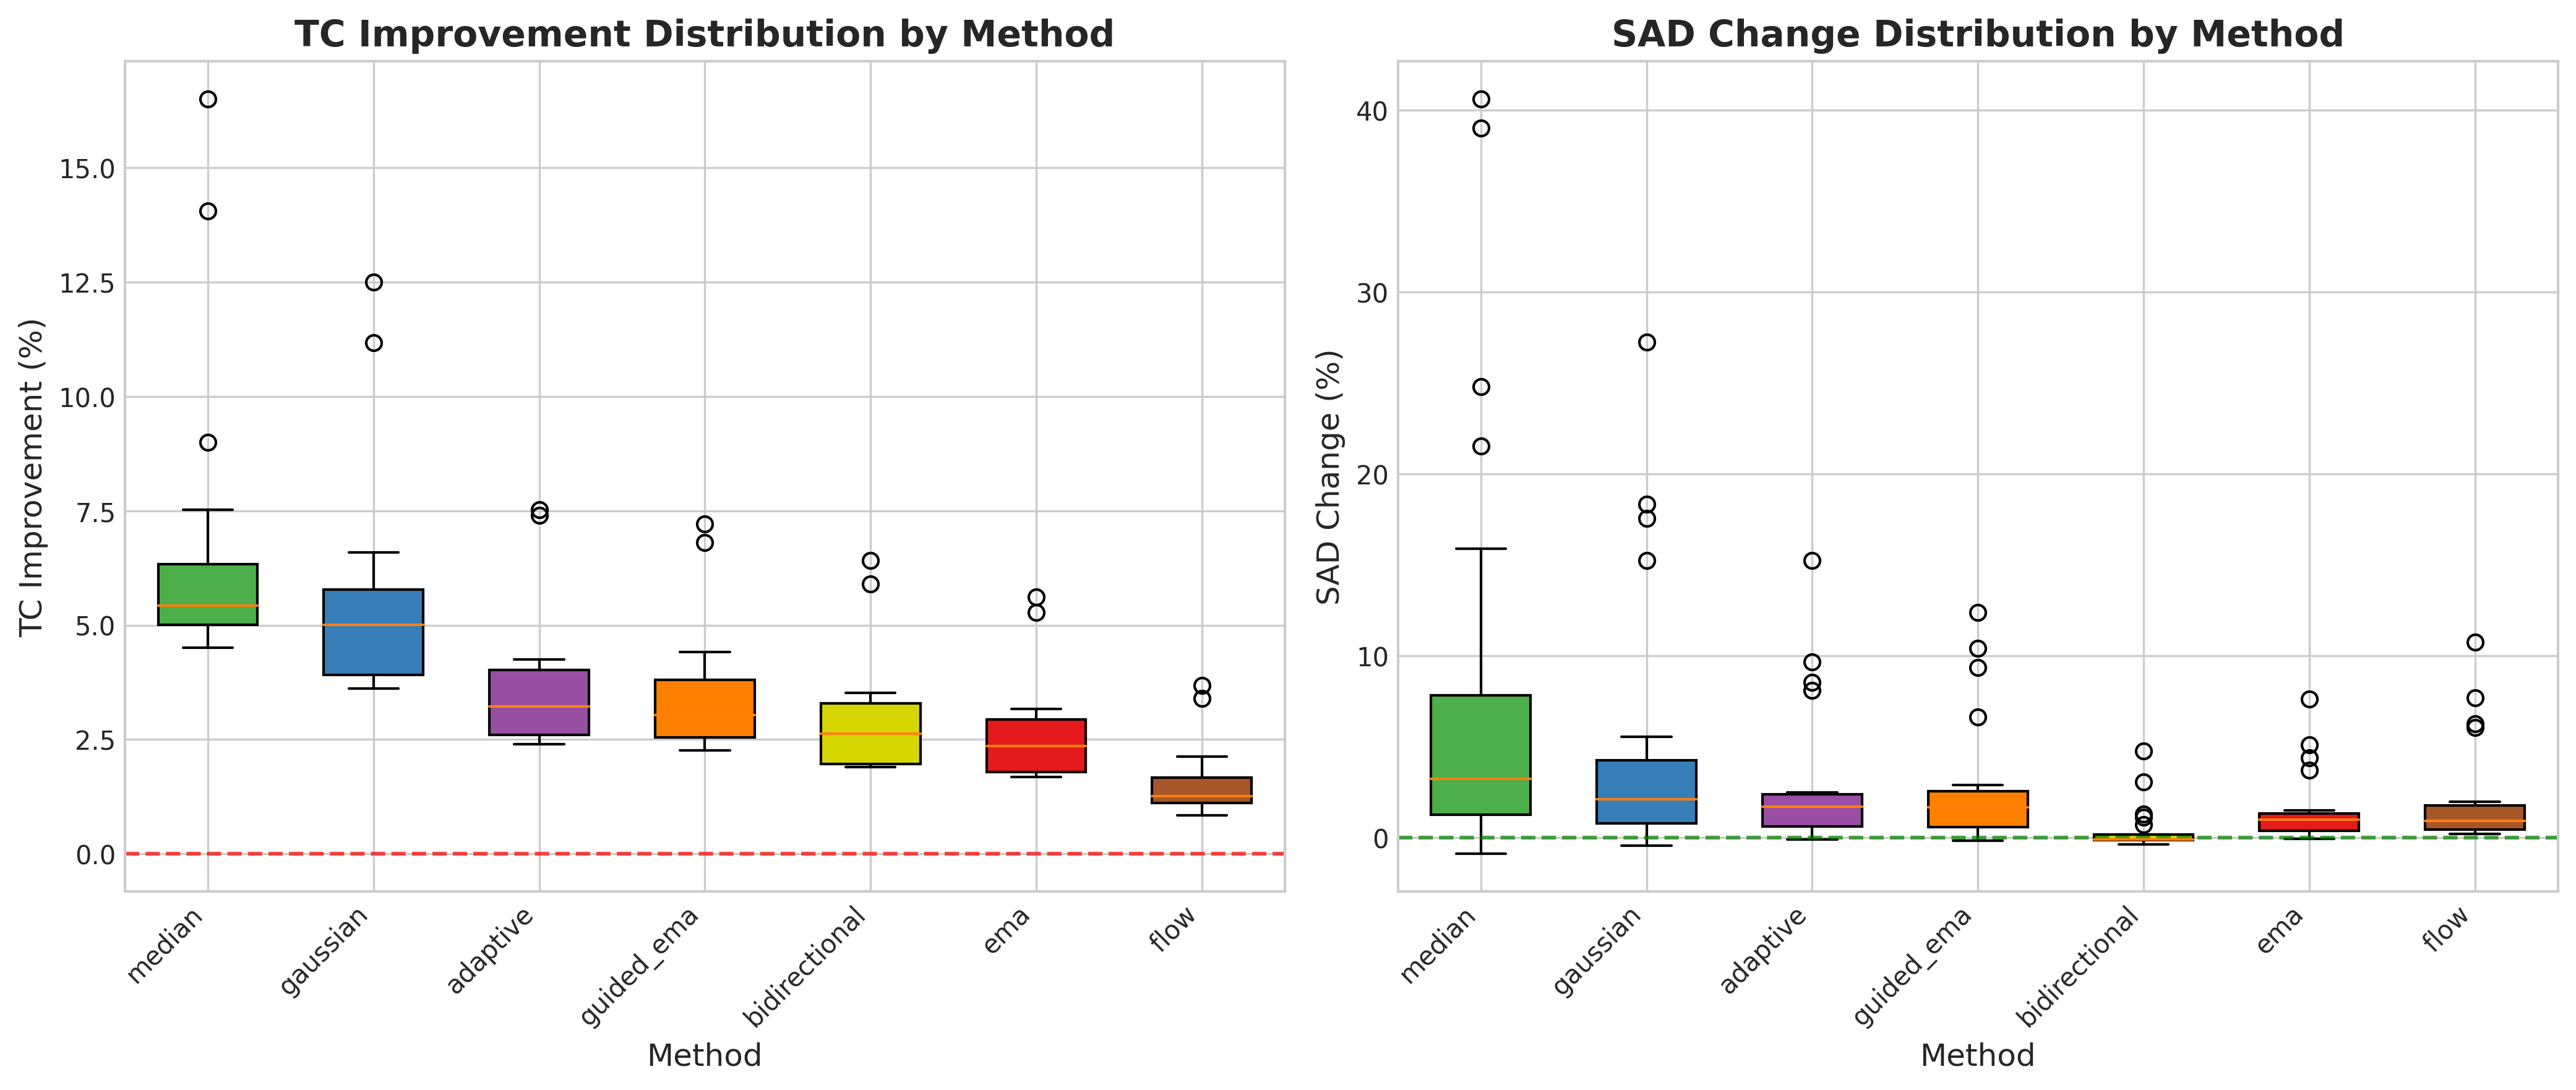
\includegraphics[width=\linewidth]{pic/figure2_method_comparison_boxplot.png}
      \vspace{0.1em}
      {\scriptsize 左：TC 提升分布 \quad | \quad 右：SAD 变化分布}
      
    \column{0.32\textwidth}
      \begin{block}{箱线图解读}
        \begin{itemize}
          \setlength{\itemsep}{0.2em}
          \item 箱体 = 四分位距（50\% 数据）
          \item 横线 = 中位数
          \item 圆形 = 异常值
        \end{itemize}
      \end{block}
      
      \vspace{0.3em}
      \begin{block}{关键观察}
        \begin{itemize}
          \setlength{\itemsep}{0.2em}
          \item \textbf{Bidirectional}：SAD 分布最集中，异常值最少
          \item \textbf{Median}：TC 提升高但波动大
          \item \textbf{Gaussian}：TC 提升分布较稳定
        \end{itemize}
      \end{block}
  \end{columns}
  
  \vspace{0.1em}
  \notestrip{nankai}{\scriptsize
  \textbf{结论：}Bidirectional 的 SAD 变化分布最集中，说明其精度表现\hilite{最稳定}，不同视频间差异最小。
  }
\end{frame}

\begin{frame}[t]{Bidirectional 平滑效果对比}
  \scriptsize
  \linespread{0.98}\selectfont
  
  \begin{columns}[T,onlytextwidth]
    \column{0.55\textwidth}
      \centering
      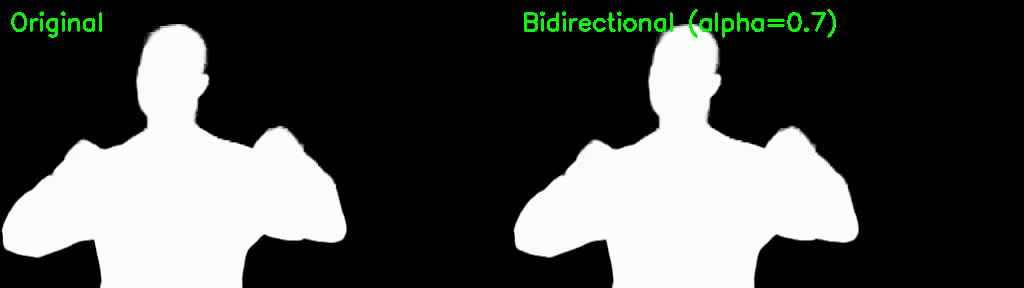
\includegraphics[width=0.98\linewidth]{pic/gif_frames/frame_0001.png}
      \vspace{0.1em}
      {\tiny 左：原始 alpha \quad | \quad 右：Bidirectional 平滑后}
      
      \vspace{0.2em}
      \href{run:pic/youtubematte_motion_0016_bidirectional_comparison_slow_hq.gif}{%
        \color{accentblue}{\underline{[Click] 点击播放动画效果 (GIF)}}%
      }
      
      \vspace{0.3em}
      \begin{block}{视觉效果}
        \begin{itemize}
          \setlength{\itemsep}{0.2em}
          \item 发丝细节\hilite{无明显模糊}
          \item 边缘抖动\hilite{明显减弱}
          \item 背景替换后\hilite{闪烁减少}
        \end{itemize}
      \end{block}
      
    \column{0.42\textwidth}
      \begin{block}{性能指标}
        \scriptsize
        \begin{tabular}{lcc}
          \toprule
          \textbf{指标} & \textbf{数值} & \textbf{评价} \\
          \midrule
          TC 提升 & 2.89\% & 提升 \\
          SAD 变化 & +0.44\% & 几乎无损 \\
          MSE 变化 & -0.12\% & 改善 \\
          \bottomrule
        \end{tabular}
      \end{block}
      
      \vspace{0.3em}
      \begin{block}{优劣分析}
        \scriptsize
        \begin{itemize}
          \setlength{\itemsep}{0.1em}
          \item \textbf{优点：}精度几乎无损，发丝细节保留完整
          \item \textbf{缺点：}TC 提升幅度相对较小
        \end{itemize}
      \end{block}
  \end{columns}
  
  \vspace{0.2em}
  \notestrip{softgreen}{\scriptsize
  \textbf{结论：}Bidirectional 在\hilite{保持视觉质量的同时}实现时序一致性提升，是精度无损场景的最佳选择。
  }
\end{frame}

\begin{frame}[t]{Median 平滑效果对比}
  \scriptsize
  \linespread{0.98}\selectfont
  
  \begin{columns}[T,onlytextwidth]
    \column{0.55\textwidth}
      \centering
      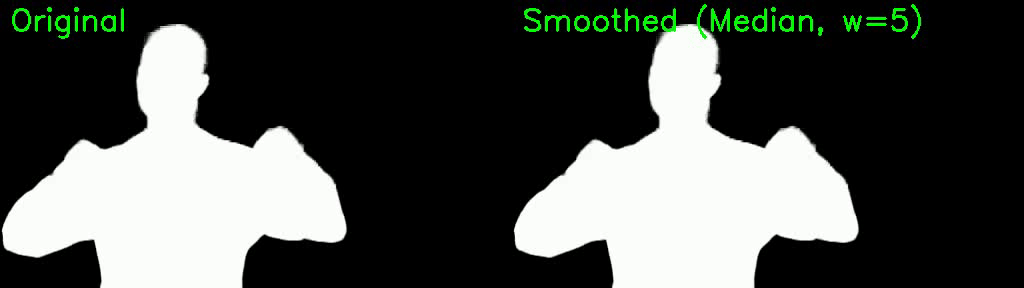
\includegraphics[width=0.98\linewidth]{pic/median_frames/median_frame_0001.png}
      \vspace{0.1em}
      {\tiny 左：原始 alpha \quad | \quad 右：Median 平滑后}
      
      \vspace{0.2em}
      \href{run:pic/youtubematte_motion_0016_comparison_slow_hq.gif}{%
        \color{accentblue}{\underline{[Click] 点击播放动画效果 (GIF)}}%
      }
      
      \vspace{0.3em}
      \begin{block}{视觉效果}
        \begin{itemize}
          \setlength{\itemsep}{0.2em}
          \item 发丝细节\hilite{明显模糊}
          \item 边缘抖动\hilite{减少但细节丢失}
          \item 背景替换后\hilite{毛边明显}
        \end{itemize}
      \end{block}
      
    \column{0.42\textwidth}
      \begin{block}{性能指标}
        \scriptsize
        \begin{tabular}{lcc}
          \toprule
          \textbf{指标} & \textbf{数值} & \textbf{评价} \\
          \midrule
          TC 提升 & 6.68\% & 提升最大 \\
          SAD 变化 & +8.88\% & 恶化严重 \\
          MSE 变化 & +23.91\% & 恶化严重 \\
          \bottomrule
        \end{tabular}
      \end{block}
      
      \vspace{0.3em}
      \begin{block}{优劣分析}
        \scriptsize
        \begin{itemize}
          \setlength{\itemsep}{0.1em}
          \item \textbf{优点：}TC 提升最大（6.68\%），时序稳定性最好
          \item \textbf{缺点：}发丝模糊严重，视觉损失不可接受
        \end{itemize}
      \end{block}
  \end{columns}
  
  \vspace{0.2em}
  \notestrip{softorange}{\scriptsize
  \textbf{结论：}Median 数值最优但\hilite{视觉损失严重}，不适合需要精细边缘的实际应用。
  }
\end{frame}


\begin{frame}[t]{Gaussian 平滑效果对比}
  \scriptsize
  \linespread{0.98}\selectfont
  
  \begin{columns}[T,onlytextwidth]
    \column{0.55\textwidth}
      \centering
      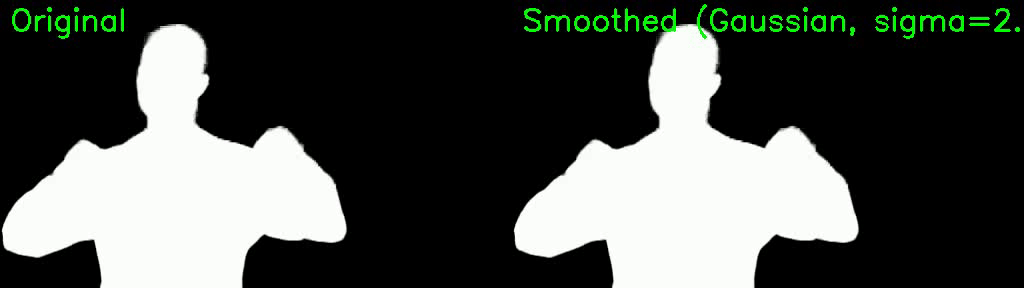
\includegraphics[width=0.98\linewidth]{pic/gaussian_frames/gaussian_frame_0001.png}
      \vspace{0.1em}
      {\tiny 左：原始 alpha \quad | \quad 右：Gaussian 平滑后 (sigma=2.0)}
      
      \vspace{0.2em}
      \href{run:pic/youtubematte_motion_0016_gaussian_comparison_slow_hq.gif}{%
        \color{accentblue}{\underline{[Click] 点击播放动画效果 (GIF)}}%
      }
      
      \vspace{0.3em}
      \begin{block}{视觉效果}
        \begin{itemize}
          \setlength{\itemsep}{0.2em}
          \item 发丝细节\hilite{轻微模糊}
          \item 边缘抖动\hilite{明显减少}
          \item 整体\hilite{平衡性较好}
        \end{itemize}
      \end{block}
      
    \column{0.42\textwidth}
      \begin{block}{性能指标}
        \scriptsize
        \begin{tabular}{lcc}
          \toprule
          \textbf{指标} & \textbf{数值} & \textbf{评价} \\
          \midrule
          TC 提升 & 4.0\% & 提升显著 \\
          SAD 变化 & +2.4\% & 轻微恶化 \\
          MSE 变化 & +3.0\% & 轻微恶化 \\
          \bottomrule
        \end{tabular}
      \end{block}
      
      \vspace{0.3em}
      \begin{block}{优劣分析}
        \scriptsize
        \begin{itemize}
          \setlength{\itemsep}{0.1em}
          \item \textbf{优点：}TC 提升显著（4.0\%），是 TC 和精度的最佳平衡点
          \item \textbf{缺点：}发丝有轻微模糊，精度略有下降
        \end{itemize}
      \end{block}
  \end{columns}
  
  \vspace{0.2em}
  \notestrip{accentblue}{\scriptsize
  \textbf{建议：}追求平衡可选 Gaussian (sigma=2.0, window=5)；追求精度无损可选 Bidirectional (alpha=0.7)。
  }
\end{frame}


\begin{frame}[t]{两个数据集上的性能对比}
  \scriptsize
  \linespread{0.98}\selectfont
  
  \begin{columns}[T,onlytextwidth]
    \column{0.7\textwidth}
      \centering
      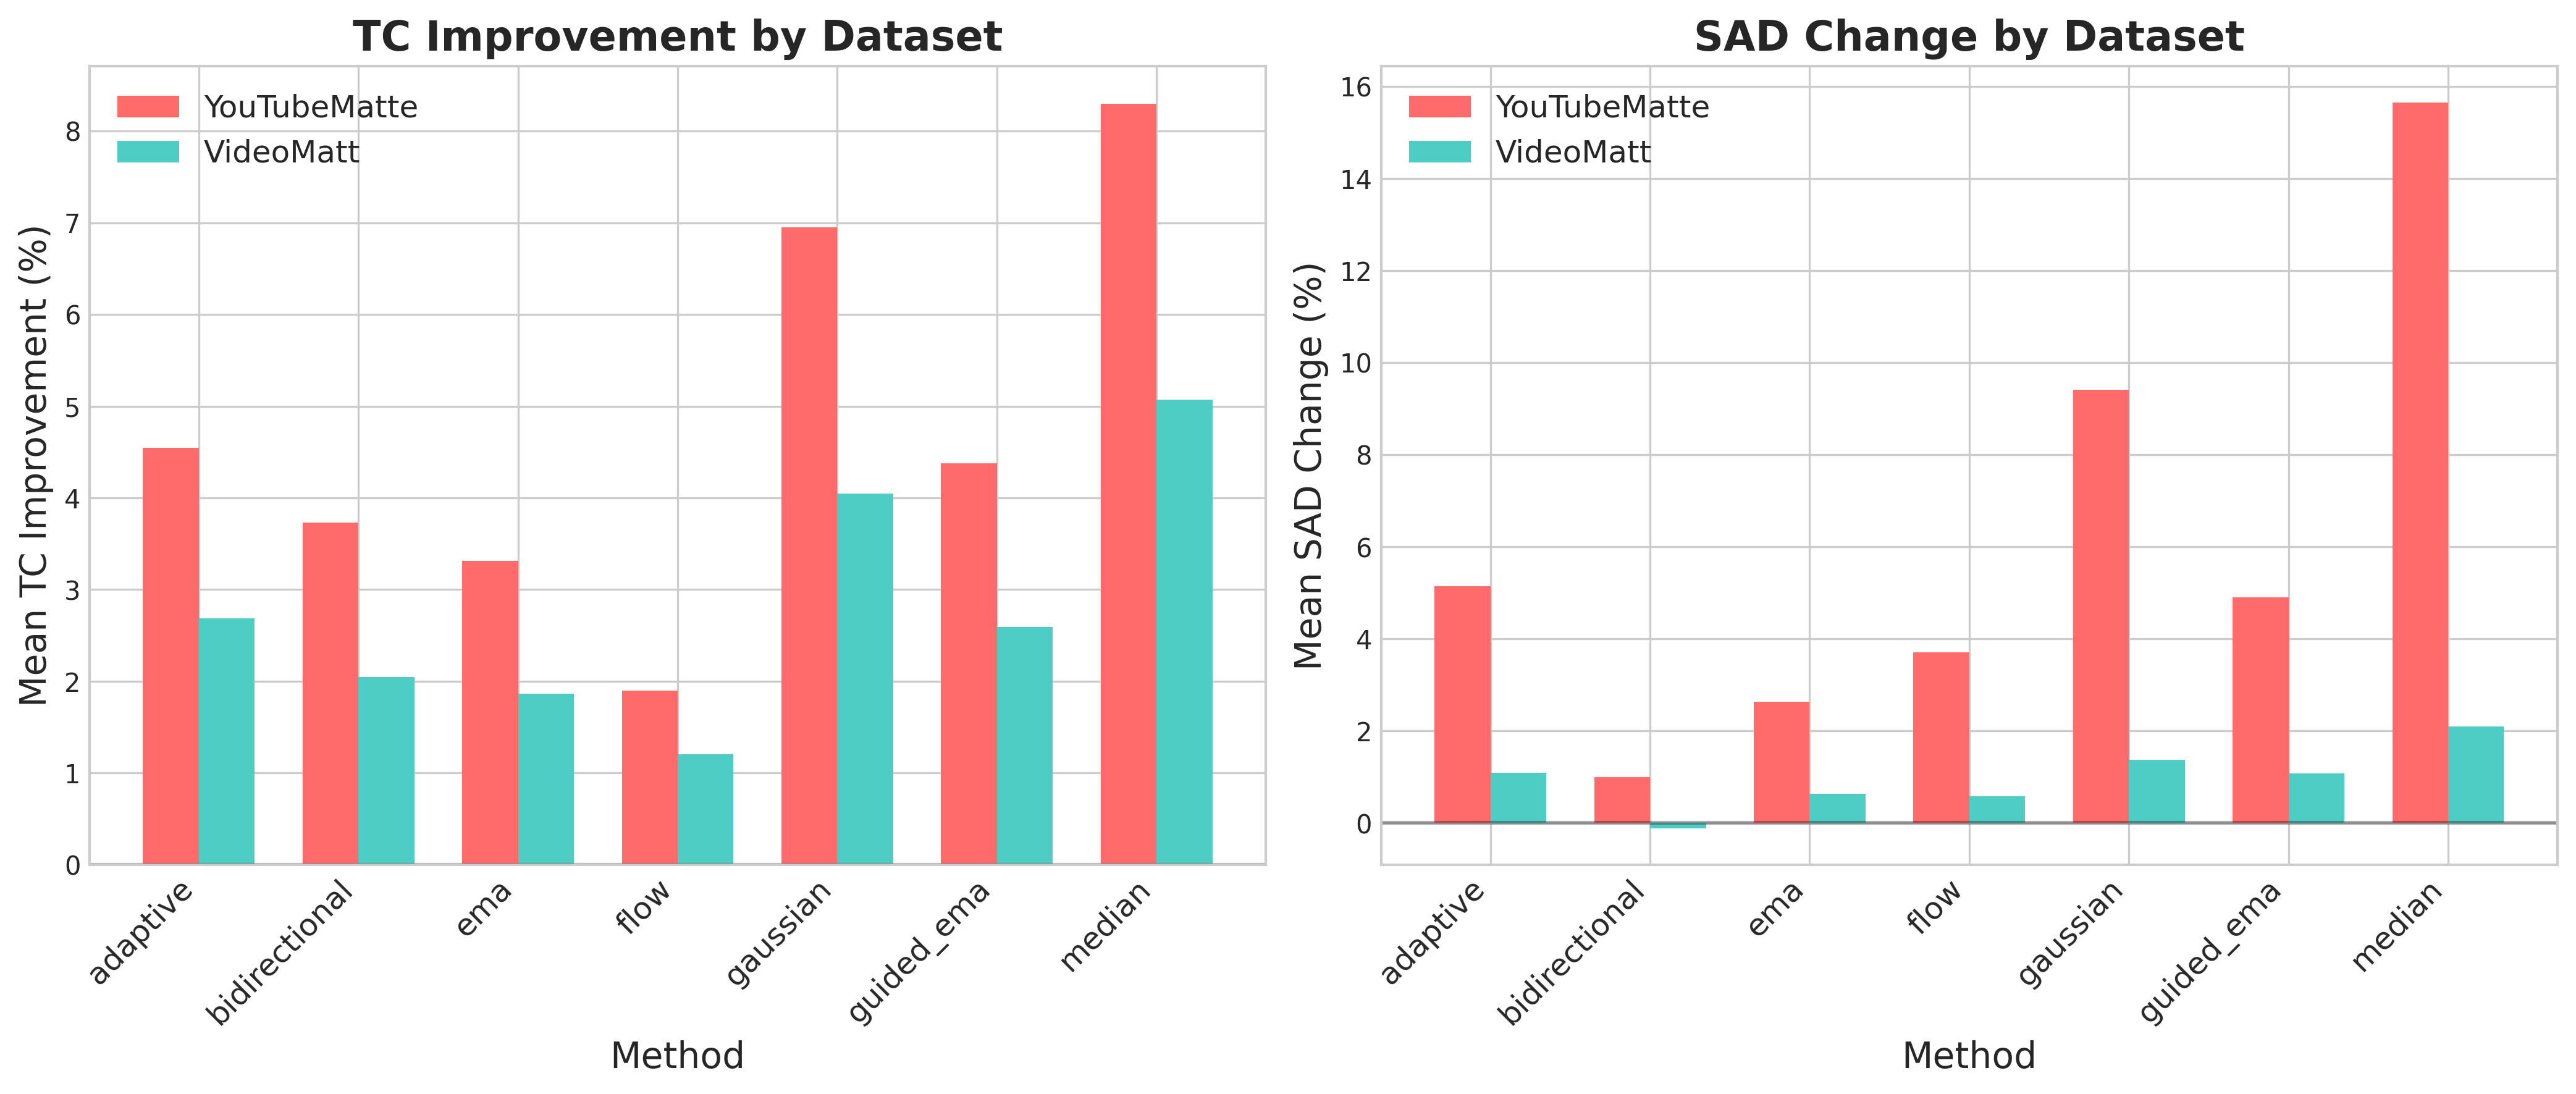
\includegraphics[width=0.98\linewidth]{pic/figure3_dataset_comparison.png}
      \vspace{0.1em}
      {\scriptsize 左：TC 提升对比 \quad | \quad 右：SAD 变化对比}
      
    \column{0.32\textwidth}
      \begin{block}{关键观察}
        \begin{itemize}
          \setlength{\itemsep}{0.2em}
          \item YouTubeMatte 上效果\hilite{普遍更好}
          \item VideoMatt 更具挑战性
          \item \textbf{Bidirectional} 表现\hilite{最稳定}
        \end{itemize}
      \end{block}
      
      \vspace{0.5em}
      \begin{block}{差异分析}
        \scriptsize
        VideoMatt 包含更多\hilite{复杂运动}和\hilite{精细结构}，平滑难度更高。
      \end{block}
    \end{columns}
   \vspace{0.1em}
  \notestrip{accentblue}{\scriptsize
  \textbf{结论：}Bidirectional 在两个数据集上表现最稳定，适合不同场景的视频抠图任务。
  }
\end{frame}

\begin{frame}[t]{Gaussian 参数敏感性分析}
  \vspace{-0.5cm}
  \scriptsize
  \linespread{0.98}\selectfont
  
  \begin{columns}[T,onlytextwidth]
    \column{0.65\textwidth}
      \centering
      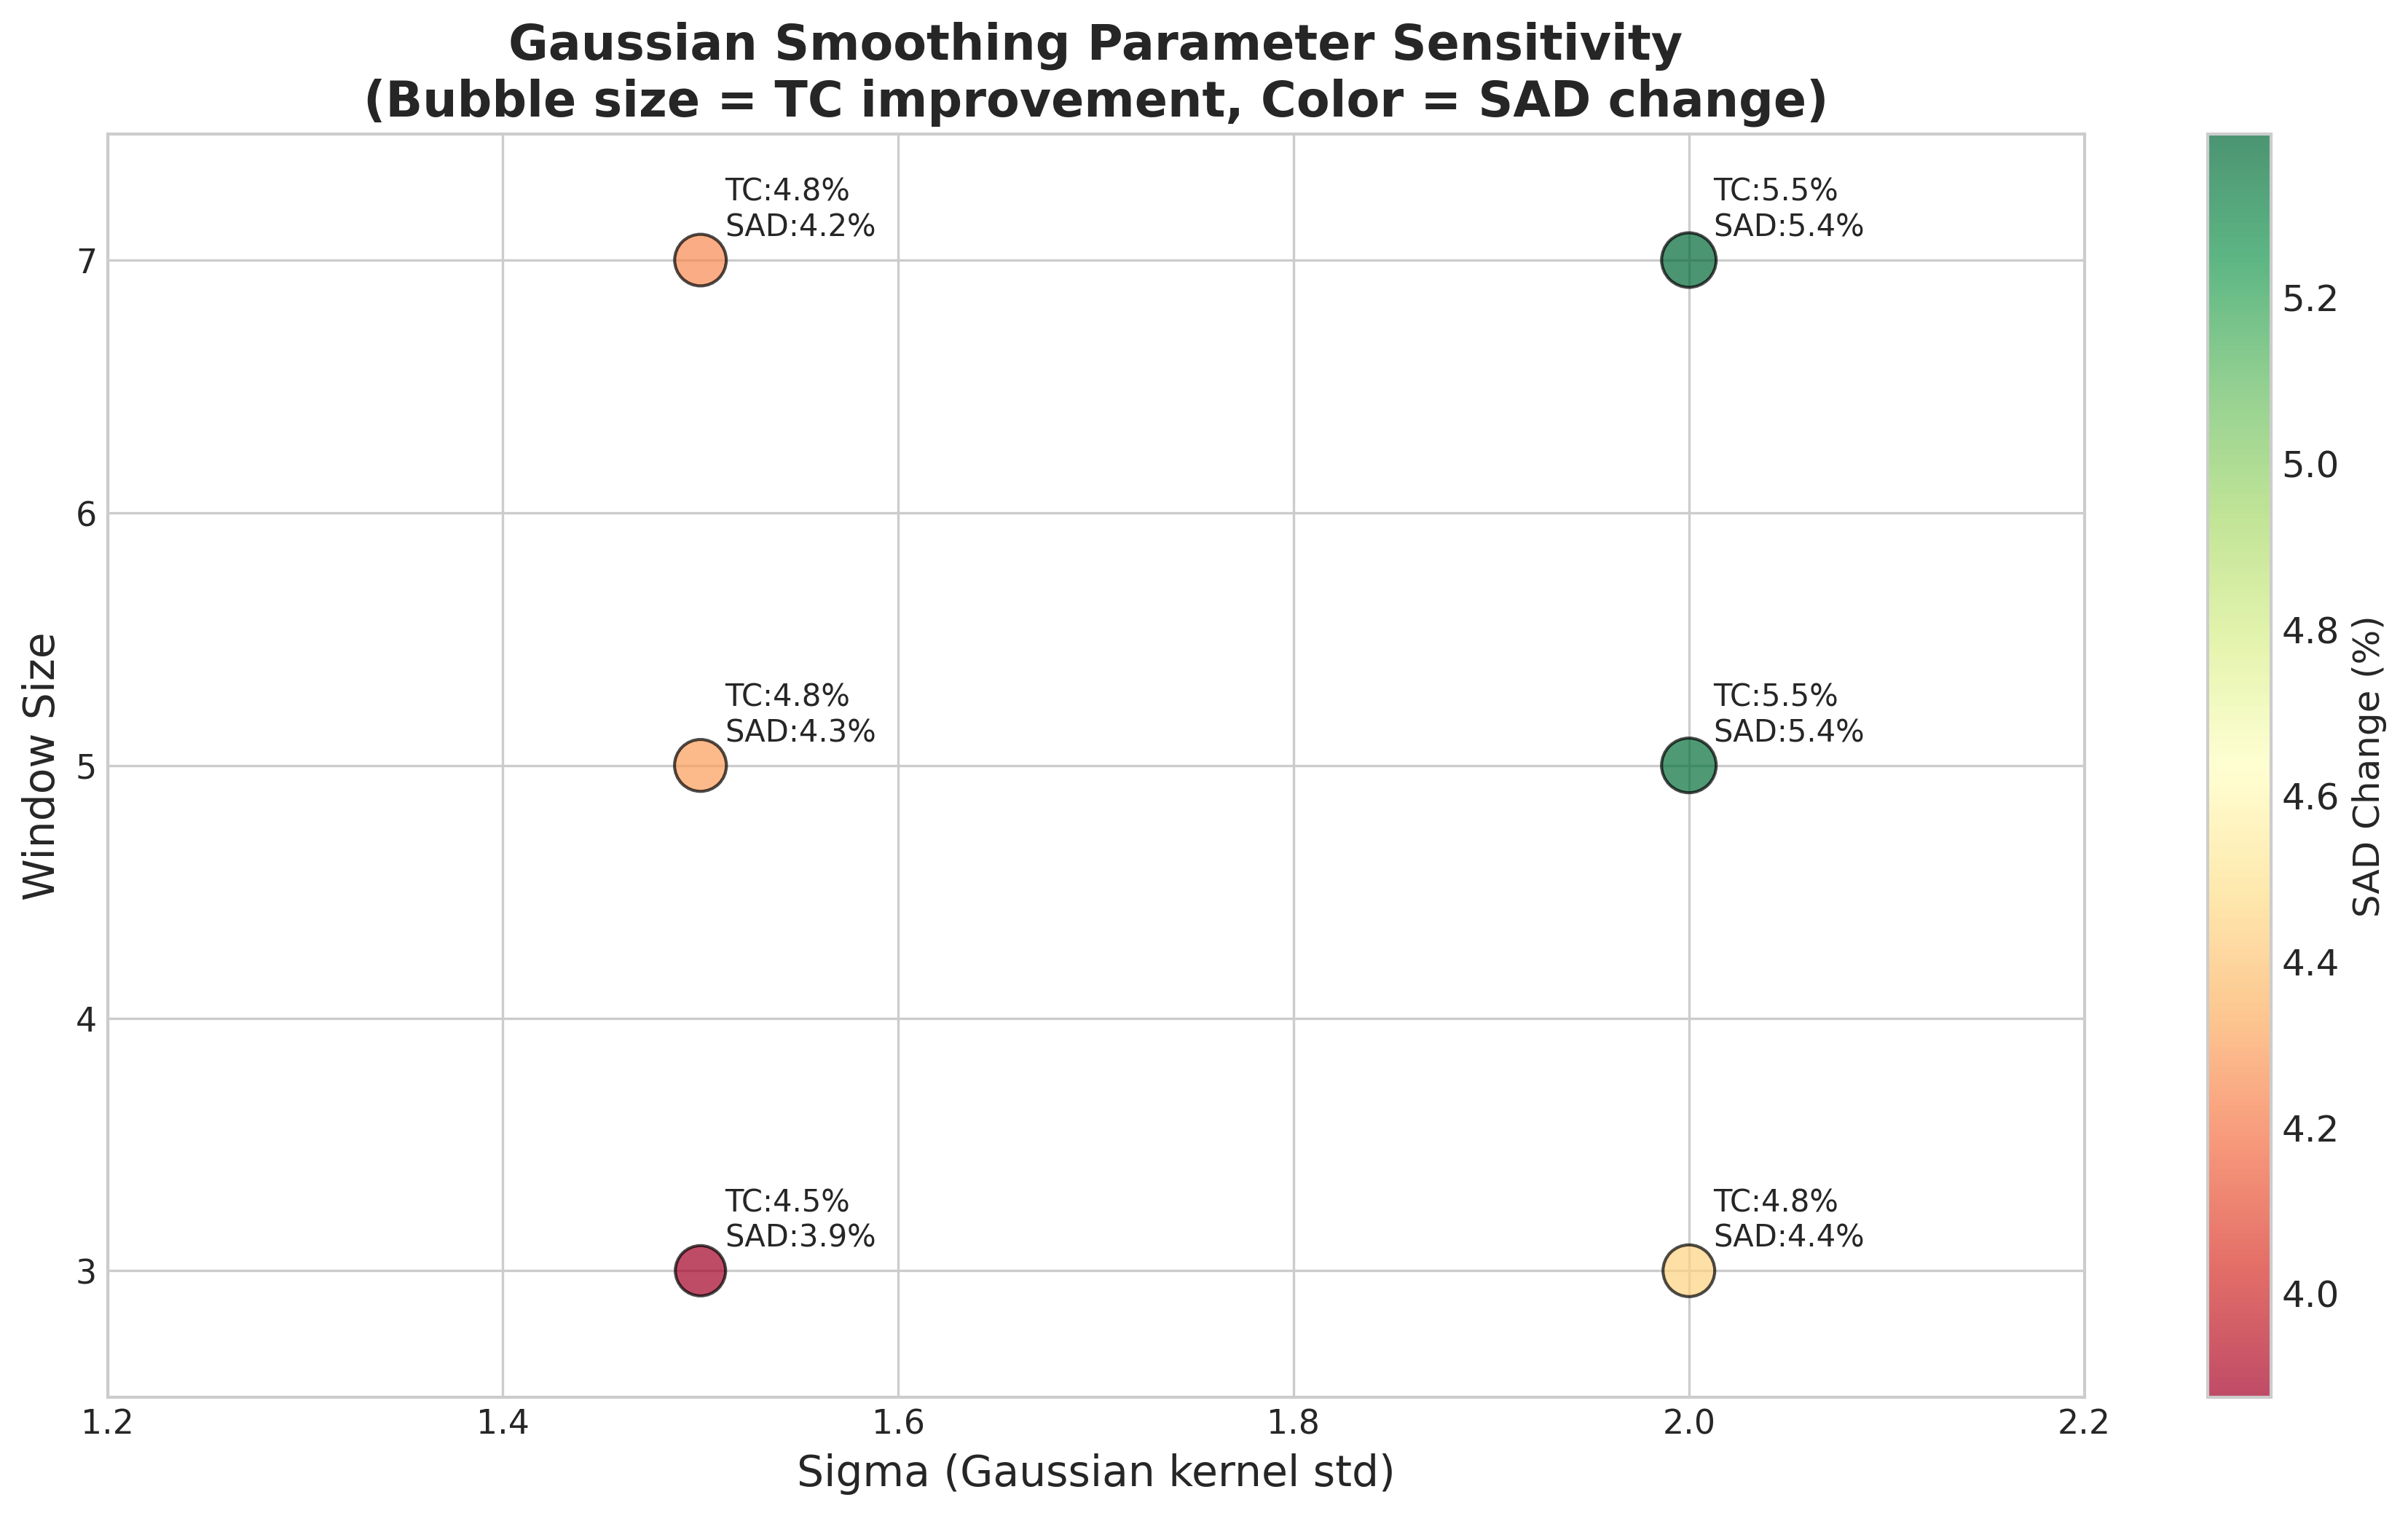
\includegraphics[width=0.98\linewidth]{pic/figure4_gaussian_parameter_sensitivity.png}
      \vspace{0.1em}
      {\scriptsize 气泡大小 = TC 提升，颜色 = SAD 变化}
      
    \column{0.32\textwidth}
      \begin{block}{参数趋势}
        \begin{itemize}
          \setlength{\itemsep}{0.2em}
          \item 增大 sigma → TC 提升增加
          \item 增大 sigma → SAD 恶化加剧
          \item 增大窗口 → 效果饱和
        \end{itemize}
      \end{block}
      
      \vspace{0.3em}
      \begin{block}{推荐参数}
        \centering
        \metricchip{softgreen}{sigma=2.0}{window=5} \\
        \vspace{0.1em}
        {\scriptsize TC 提升: 4.0\%, SAD 增加: 2.4\%}
      \end{block}
  \end{columns}
  
  \vspace{0.1em}
  \notestrip{accentblue}{\scriptsize
  \textbf{建议：}追求平衡可选 Gaussian；追求精度无损可选 Bidirectional。
  }
\end{frame}

\begin{frame}[t]{综合性能雷达图}
  \vspace{-0.5cm}
  \scriptsize
  \linespread{0.98}\selectfont
  
  \begin{columns}[T,onlytextwidth]
    \column{0.60\textwidth}
      \centering
      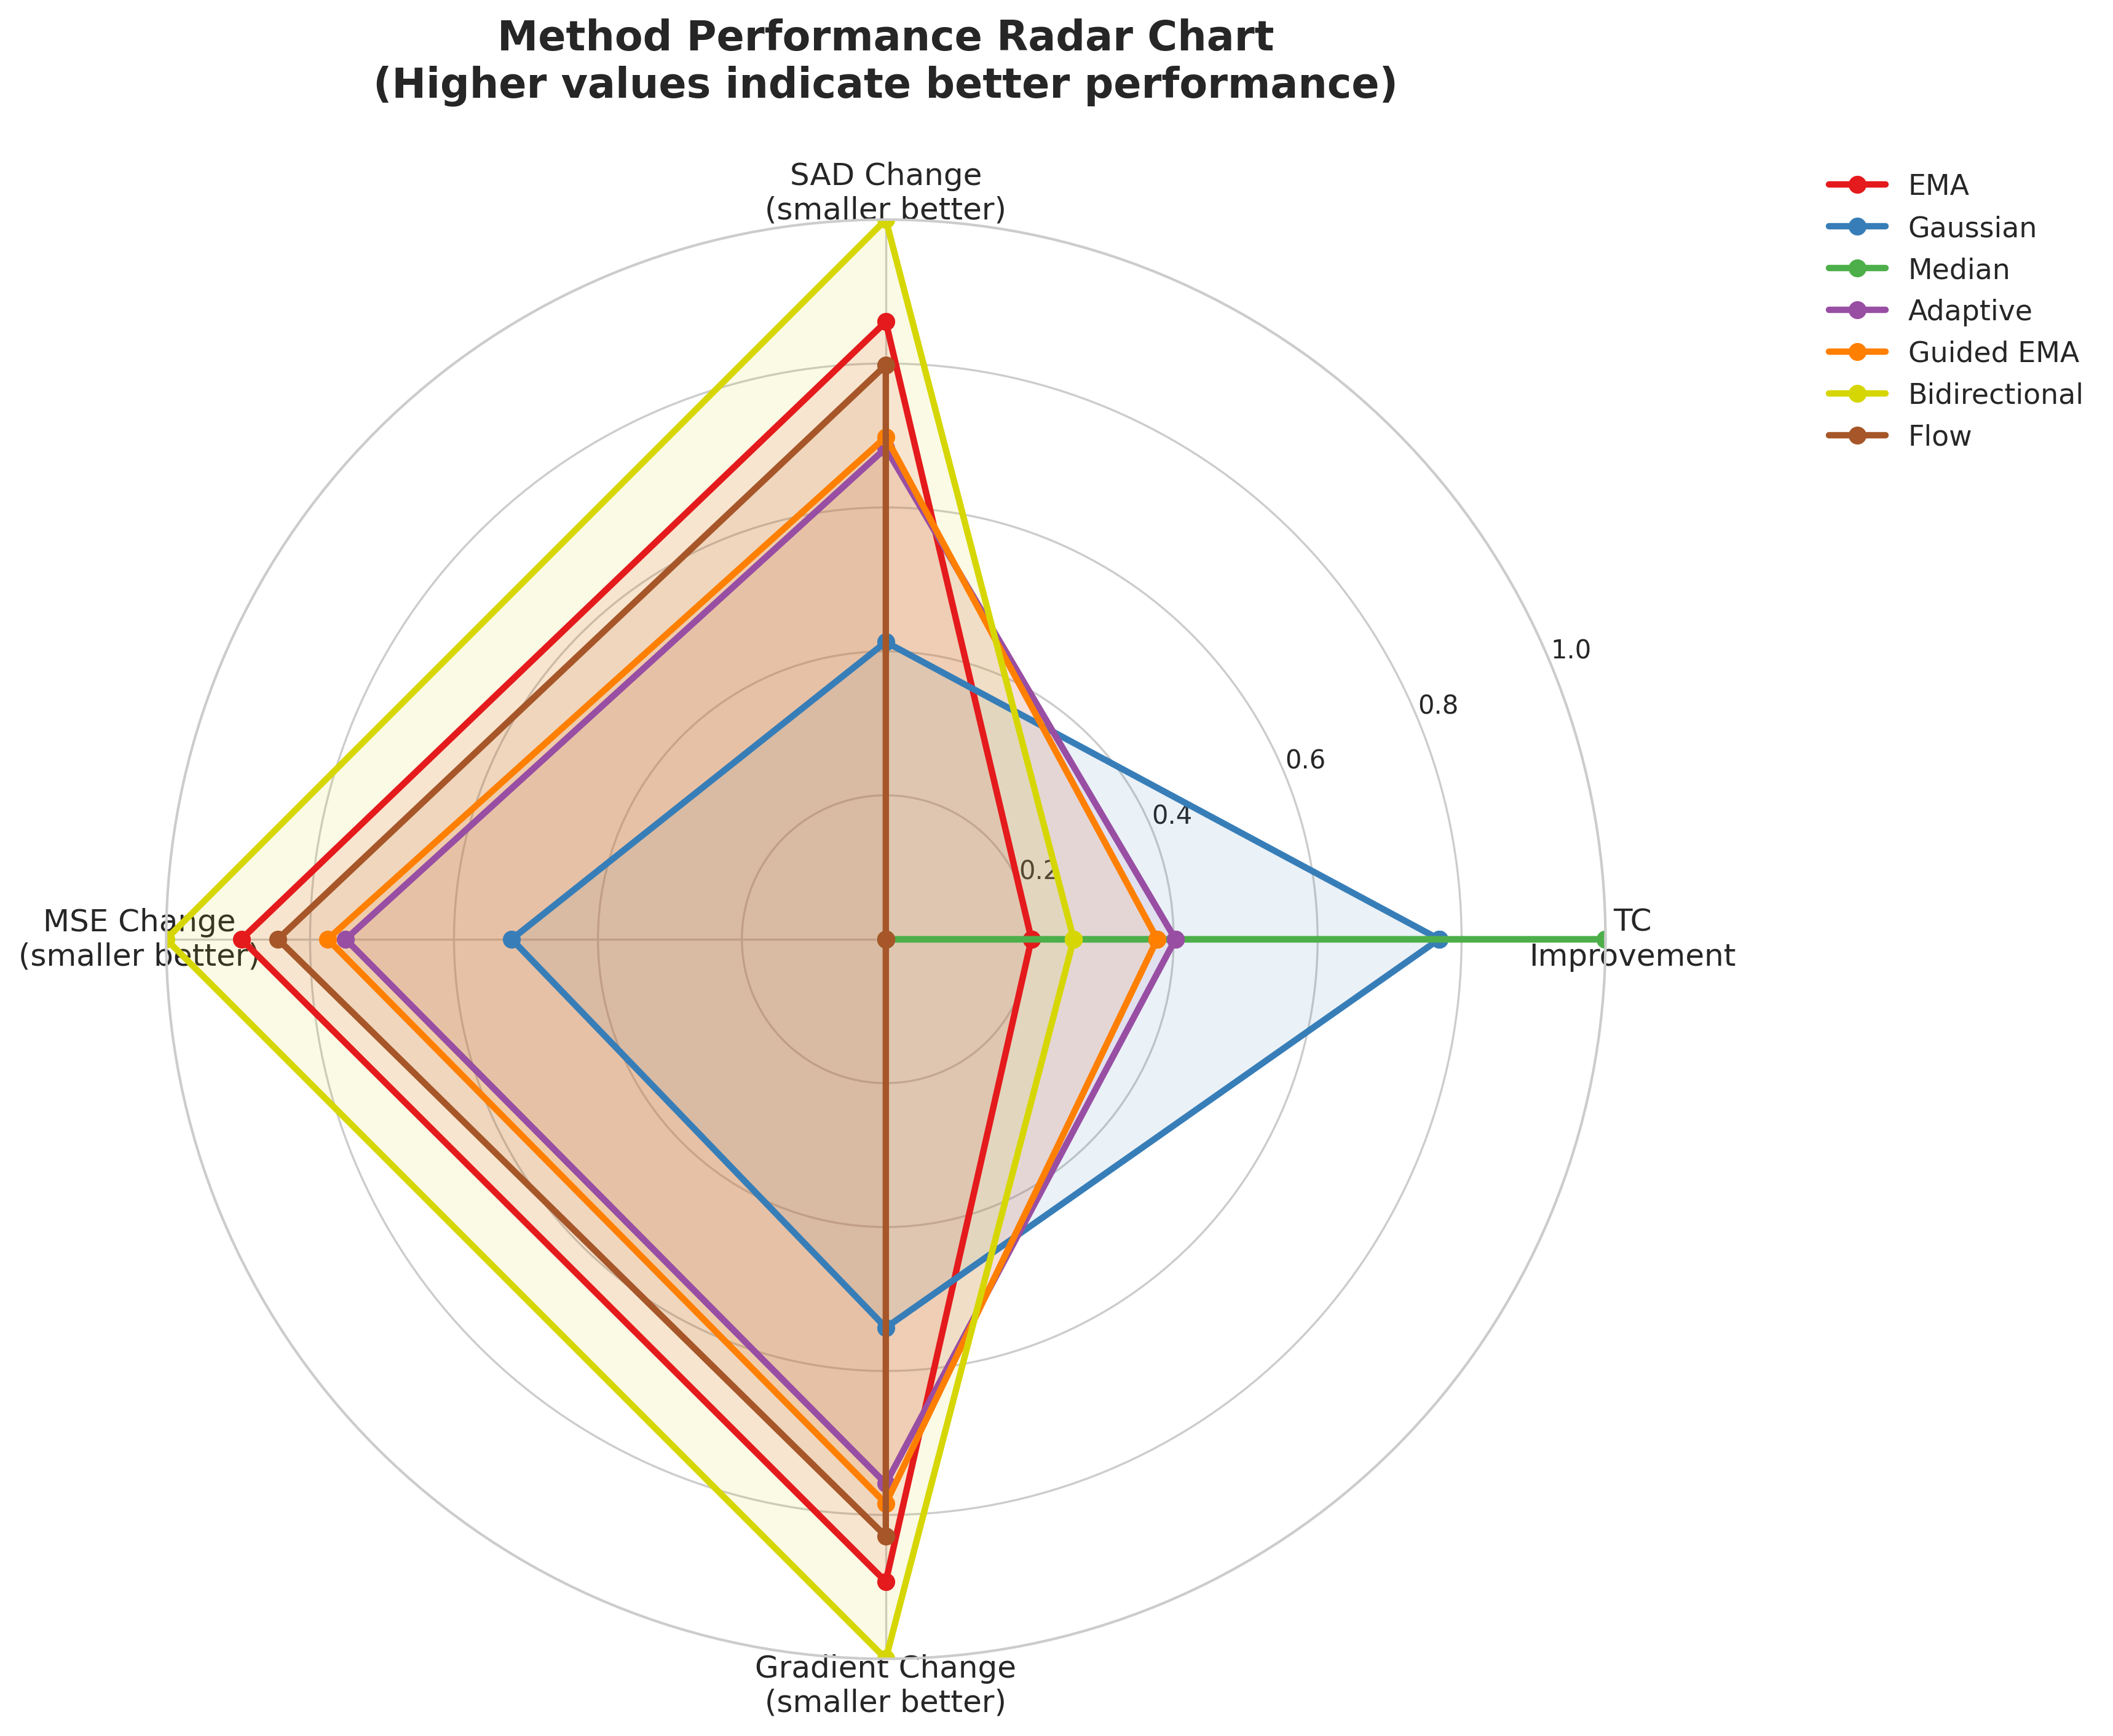
\includegraphics[width=0.95\linewidth]{pic/figure5_radar_chart.png}
      
    \column{0.32\textwidth}
      \begin{block}{解读}
        \begin{itemize}
          \setlength{\itemsep}{0.2em}
          \item 雷达图中 SAD/MSE/Gradient 已反向归一化，\hilite{值越大 = 性能越好}。
          \item \textbf{Bidirectional} 最均衡
          \item Median 偏科严重
        \end{itemize}
      \end{block}
      
      \vspace{0.3em}
      \begin{block}{总结}
        \centering
        \textbf{Bidirectional (alpha=0.7)} \\
        \vspace{0.1em}
        → 雷达图面积最大 \\
        → 推荐为默认平滑策略
      \end{block}
  \end{columns}
  
  
\end{frame}

\begin{frame}[t]{视频换背景 Demo}
  \scriptsize
  \linespread{0.98}\selectfont
  
  \begin{columns}[T,onlytextwidth]
    \column{0.48\textwidth}
      \begin{block}{平滑后 alpha 对比}
        \centering
        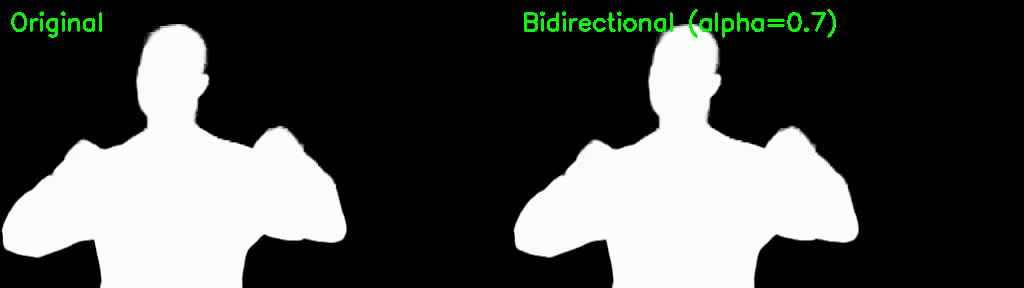
\includegraphics[width=0.95\linewidth]{pic/gif_frames/frame_0001.png}
        \vspace{0.1em}
        {\scriptsize 左：原始 \quad | \quad 右：Bidirectional 平滑后}
        
        \vspace{0.2em}
        \href{run:pic/youtubematte_motion_0016_bidirectional_slow_hq.gif}{%
          \color{accentblue}{\underline{[Click] 播放动画效果 (GIF)}}%
        }
      \end{block}
      
    \column{0.48\textwidth}
      \begin{block}{换背景效果}
        \centering
        
\includegraphics[width=0.35\linewidth]{pic/background.jpg}
        \vspace{0.1em}
        \\
        {\scriptsize 平滑后 alpha → RGBA → 背景替换}
        
        \vspace{0.2em}
        \href{run:pic/youtubematte_motion_0016_bidirectional_composer.mp4}{%
          \color{accentblue}{\underline{[Click] 播放换背景动画 (mp4)}}%
        }
      \end{block}
  \end{columns}
  
  \vspace{0.2em}
  \begin{block}{接口说明}
    \scriptsize
    \textbf{输入：}图像主线首帧 alpha / mask
    \textbf{处理：}MatAnyone2 + Bidirectional 时序平滑 (alpha=0.7)
    \textbf{输出：}逐帧稳定 alpha + 换背景合成视频
  \end{block}
  
  \vspace{0.1em}
  \notestrip{softgreen}{\scriptsize
  \textbf{效果：}Bidirectional 平滑后，背景替换视频的\hilite{边界闪烁明显减少}，同时\hilite{发丝细节保持清晰}。
  }
\end{frame} 引入，
%    继承主文件导言区的全部宏 / 配色 / 字体，无需自带 \documentclass 或 \begin{document}。
%  · 直接在下面增删 \begin{frame}[t]{标题} ... \end{frame} 即可。
%  · 可复用样式：
%       \hilite{} \tcard{} \ccard{} \notestrip{} \metricchip{} \mpill[] \pill[]
%     可选 accent：nankai、accentblue、softgreen、softorange、softgray、deepred
% ============================================================================

\section{视频与应用}

\begin{frame}[t]{视频抠图与时序平滑}
  \scriptsize
  \linespread{0.98}\selectfont
  
  \begin{columns}[T,onlytextwidth]
    \column{0.48\textwidth}
      \begin{block}{问题：视频 alpha 抖动}
        \begin{itemize}
          \setlength{\itemsep}{0.2em}
          \item MatAnyone2~{\scriptsize[7]} 逐帧推理时，alpha 存在帧间\hilite{抖动与边界闪烁}；
          \item 直接替换背景会放大这些不稳定，导致视觉不自然；
          \item 需要一种\hilite{保持细节}的时序平滑策略。
        \end{itemize}
      \end{block}
      
      \vspace{0.2em}
      \begin{block}{解决方案：边界带时序平滑}
        \centering
        \resizebox{0.95\linewidth}{!}{%
        \begin{tikzpicture}[
          >={Latex[length=2.5mm,width=2mm]},
          node distance=3mm,
          every node/.style={font=\scriptsize},
          vcard/.style={rounded corners=2pt, line width=0.8pt, align=center, inner sep=3pt},
          vblue/.style={vcard, draw=accentblue!82!black, fill=accentblue!12},
          vpurple/.style={vcard, draw=nankai!88!black, fill=nankai!12},
          vgreen/.style={vcard, draw=softgreen!72!black, fill=softgreen!14},
          varrow/.style={-{Latex[length=2.5mm,width=2mm]}, line width=1.2pt, draw=nankai!80!black}
        ]
          \node[vblue] (input) {\textbf{输入}\\alpha video};
          \node[vpurple, right=of input] (detect) {\textbf{边界检测}\\$0.05<\alpha<0.95$};
          \node[vgreen, right=of detect] (smooth) {\textbf{时序平滑}\\EMA / Bidirectional};
          \node[vblue, right=of smooth] (output) {\textbf{输出}\\稳定 alpha};
          \draw[varrow] (input) -- (detect);
          \draw[varrow] (detect) -- (smooth);
          \draw[varrow] (smooth) -- (output);
        \end{tikzpicture}}
        
        \vspace{0.2em}
        \scriptsize
        仅在边界区域（$\alpha\in[0.05,0.95]$）施加平滑，\hilite{保护前景核区与背景}，避免过度模糊。
      \end{block}
      
    \column{0.48\textwidth}
      \begin{block}{7 种平滑策略对比}
        \centering
        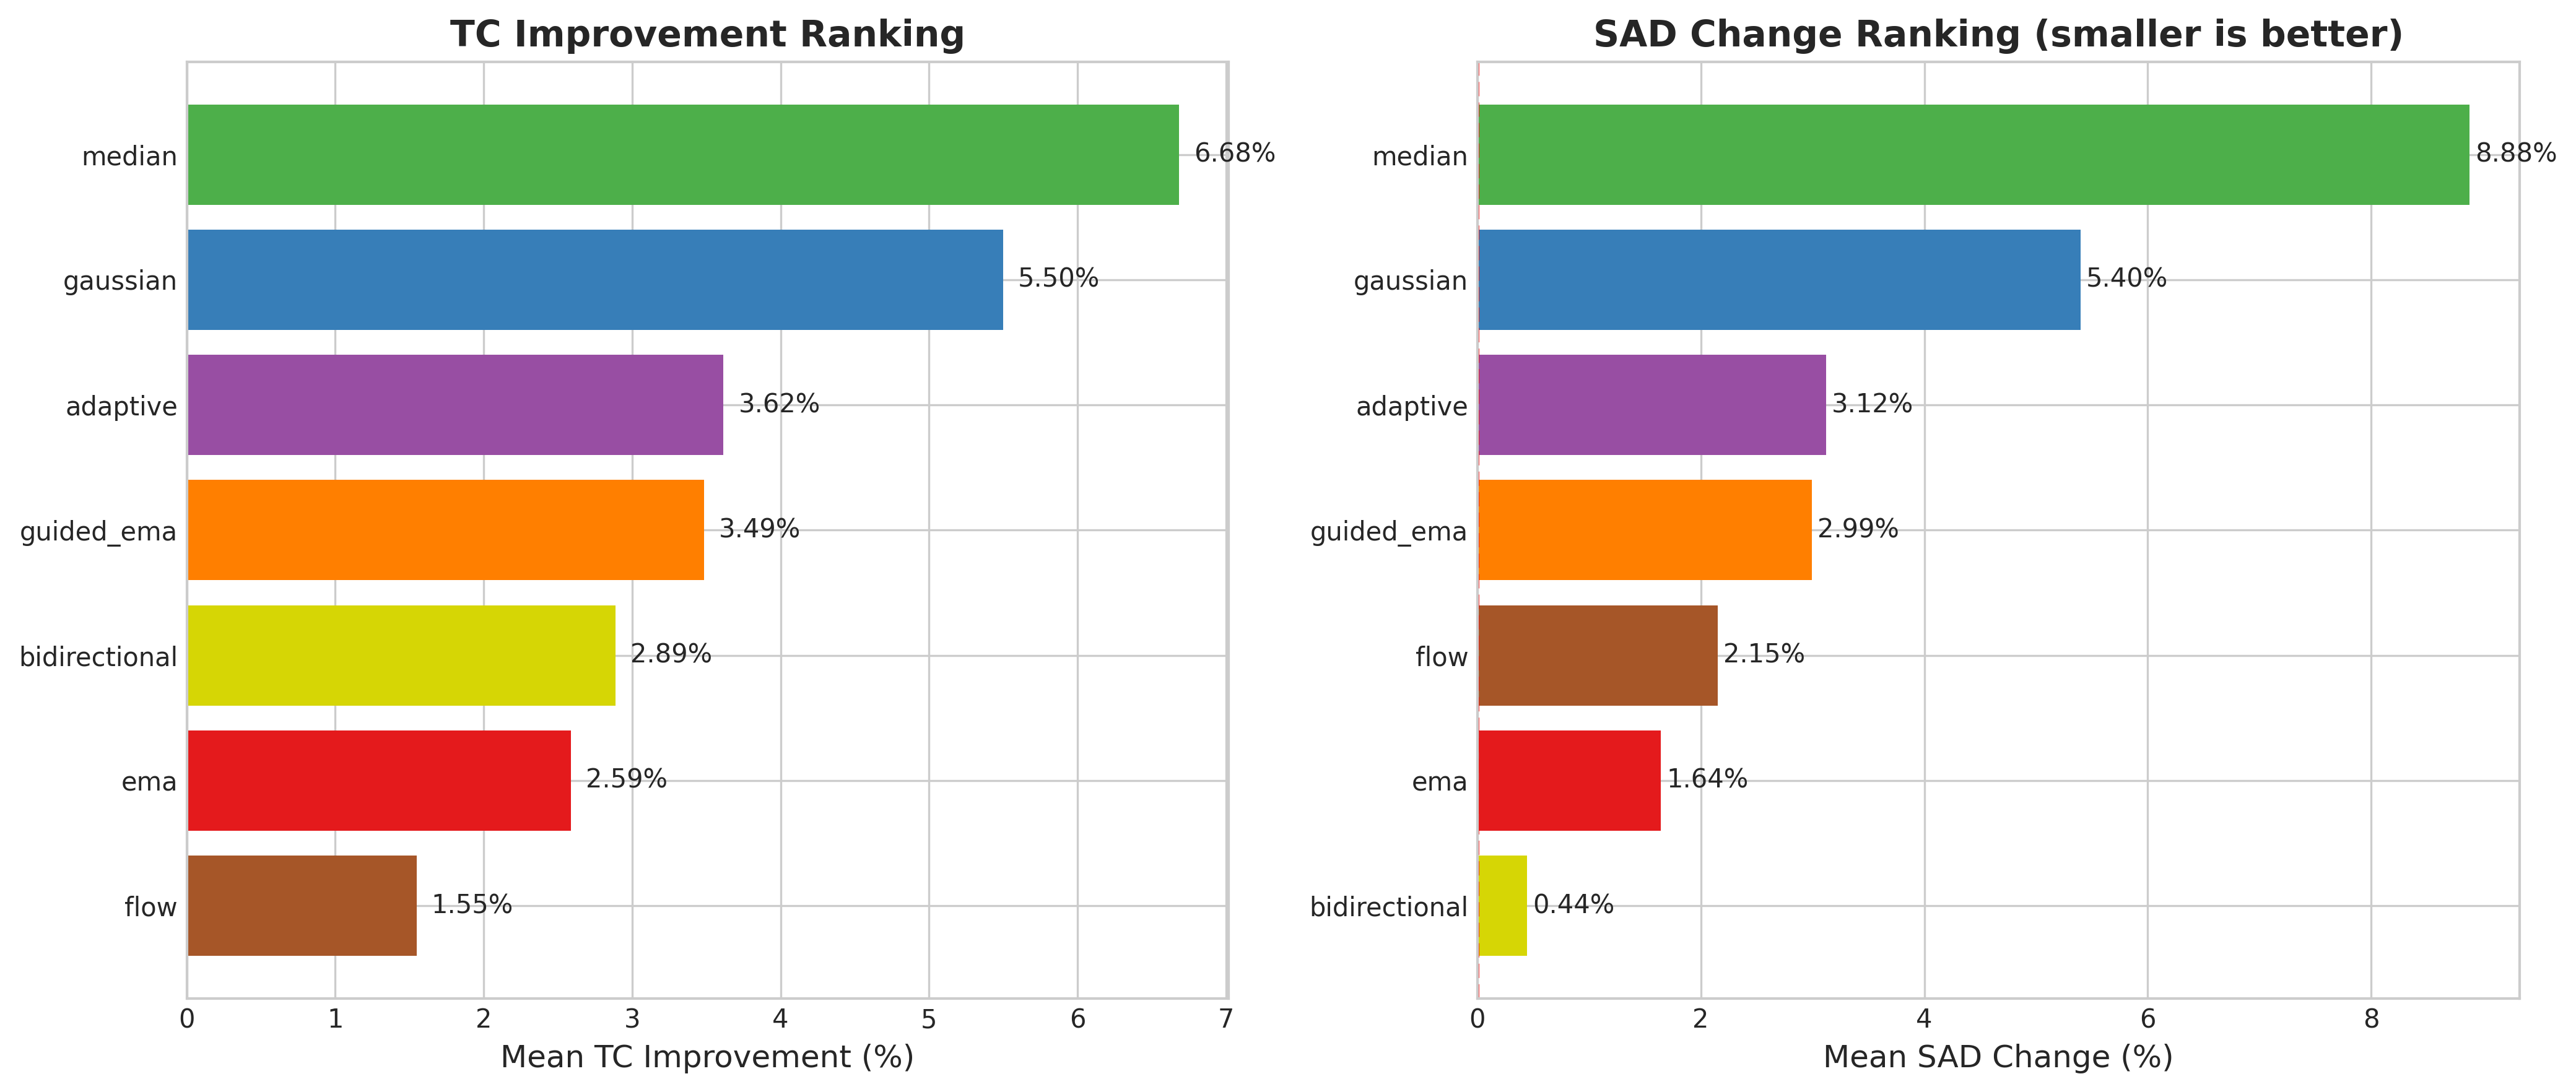
\includegraphics[width=0.95\linewidth]{pic/figure6_performance_ranking.png}
        \vspace{0.1em}
        {\scriptsize TC 提升排名（左）与 SAD 变化排名（右）}
      \end{block}
  \end{columns}
\end{frame}

\begin{frame}[t]{7 种平滑策略性能评估}
  \scriptsize
  \linespread{0.50}\selectfont
  
  \begin{block}{实验设置}
    \scriptsize
    \begin{itemize}
      \setlength{\itemsep}{0.1em}
      \item \textbf{数据集：}YouTubeMatte (10 视频) + VideoMatt (10 视频)，共 20 个测试视频；
      \item \textbf{评估指标：}TC（时序一致性）、SAD（绝对误差和）、MSE、Gradient；
      \item \textbf{方法：}EMA、Gaussian、Median、Adaptive、Guided EMA、Bidirectional、Flow。
    \end{itemize}
  \end{block}
  
  \vspace{0.1em}
  \centering
  \resizebox{0.9\linewidth}{!}{%
  \begin{tabular}{lcccc}
    \toprule
    \textbf{方法} & \textbf{TC 提升 (\%)} & \textbf{SAD 变化 (\%)} & \textbf{MSE 变化 (\%)} & \textbf{细节保留} \\
    \midrule
    Median & 6.68 & +8.88 & +23.91 & Poor \\
    Gaussian & 5.50 & +5.40 & +11.42 & Fair \\
    Adaptive & 3.62 & +3.12 & +5.88 & Fair \\
    Guided EMA & 3.49 & +2.99 & +5.28 & Fair \\
    \textbf{Bidirectional} & \textbf{2.89} & \textbf{+0.44} & \textbf{-0.12} & \textbf{Excellent} \\
    EMA & 2.59 & +1.64 & +2.40 & Good \\
    Flow & 1.55 & +2.15 & +3.62 & Fair \\
    \bottomrule
  \end{tabular}}
  
  
  \vspace{0.1em}
  \notestrip{nankai}{\scriptsize
  \textbf{关键发现：}Bidirectional 是\hilite{唯一能同时改善 TC 和保持精度}的方法，细节保留最佳。
  }
\end{frame}

\begin{frame}[t]{方法对比散点图}
  \scriptsize
  \linespread{0.92}\selectfont
  
  \begin{columns}[T,onlytextwidth]
    \column{0.60\textwidth}
      \centering
      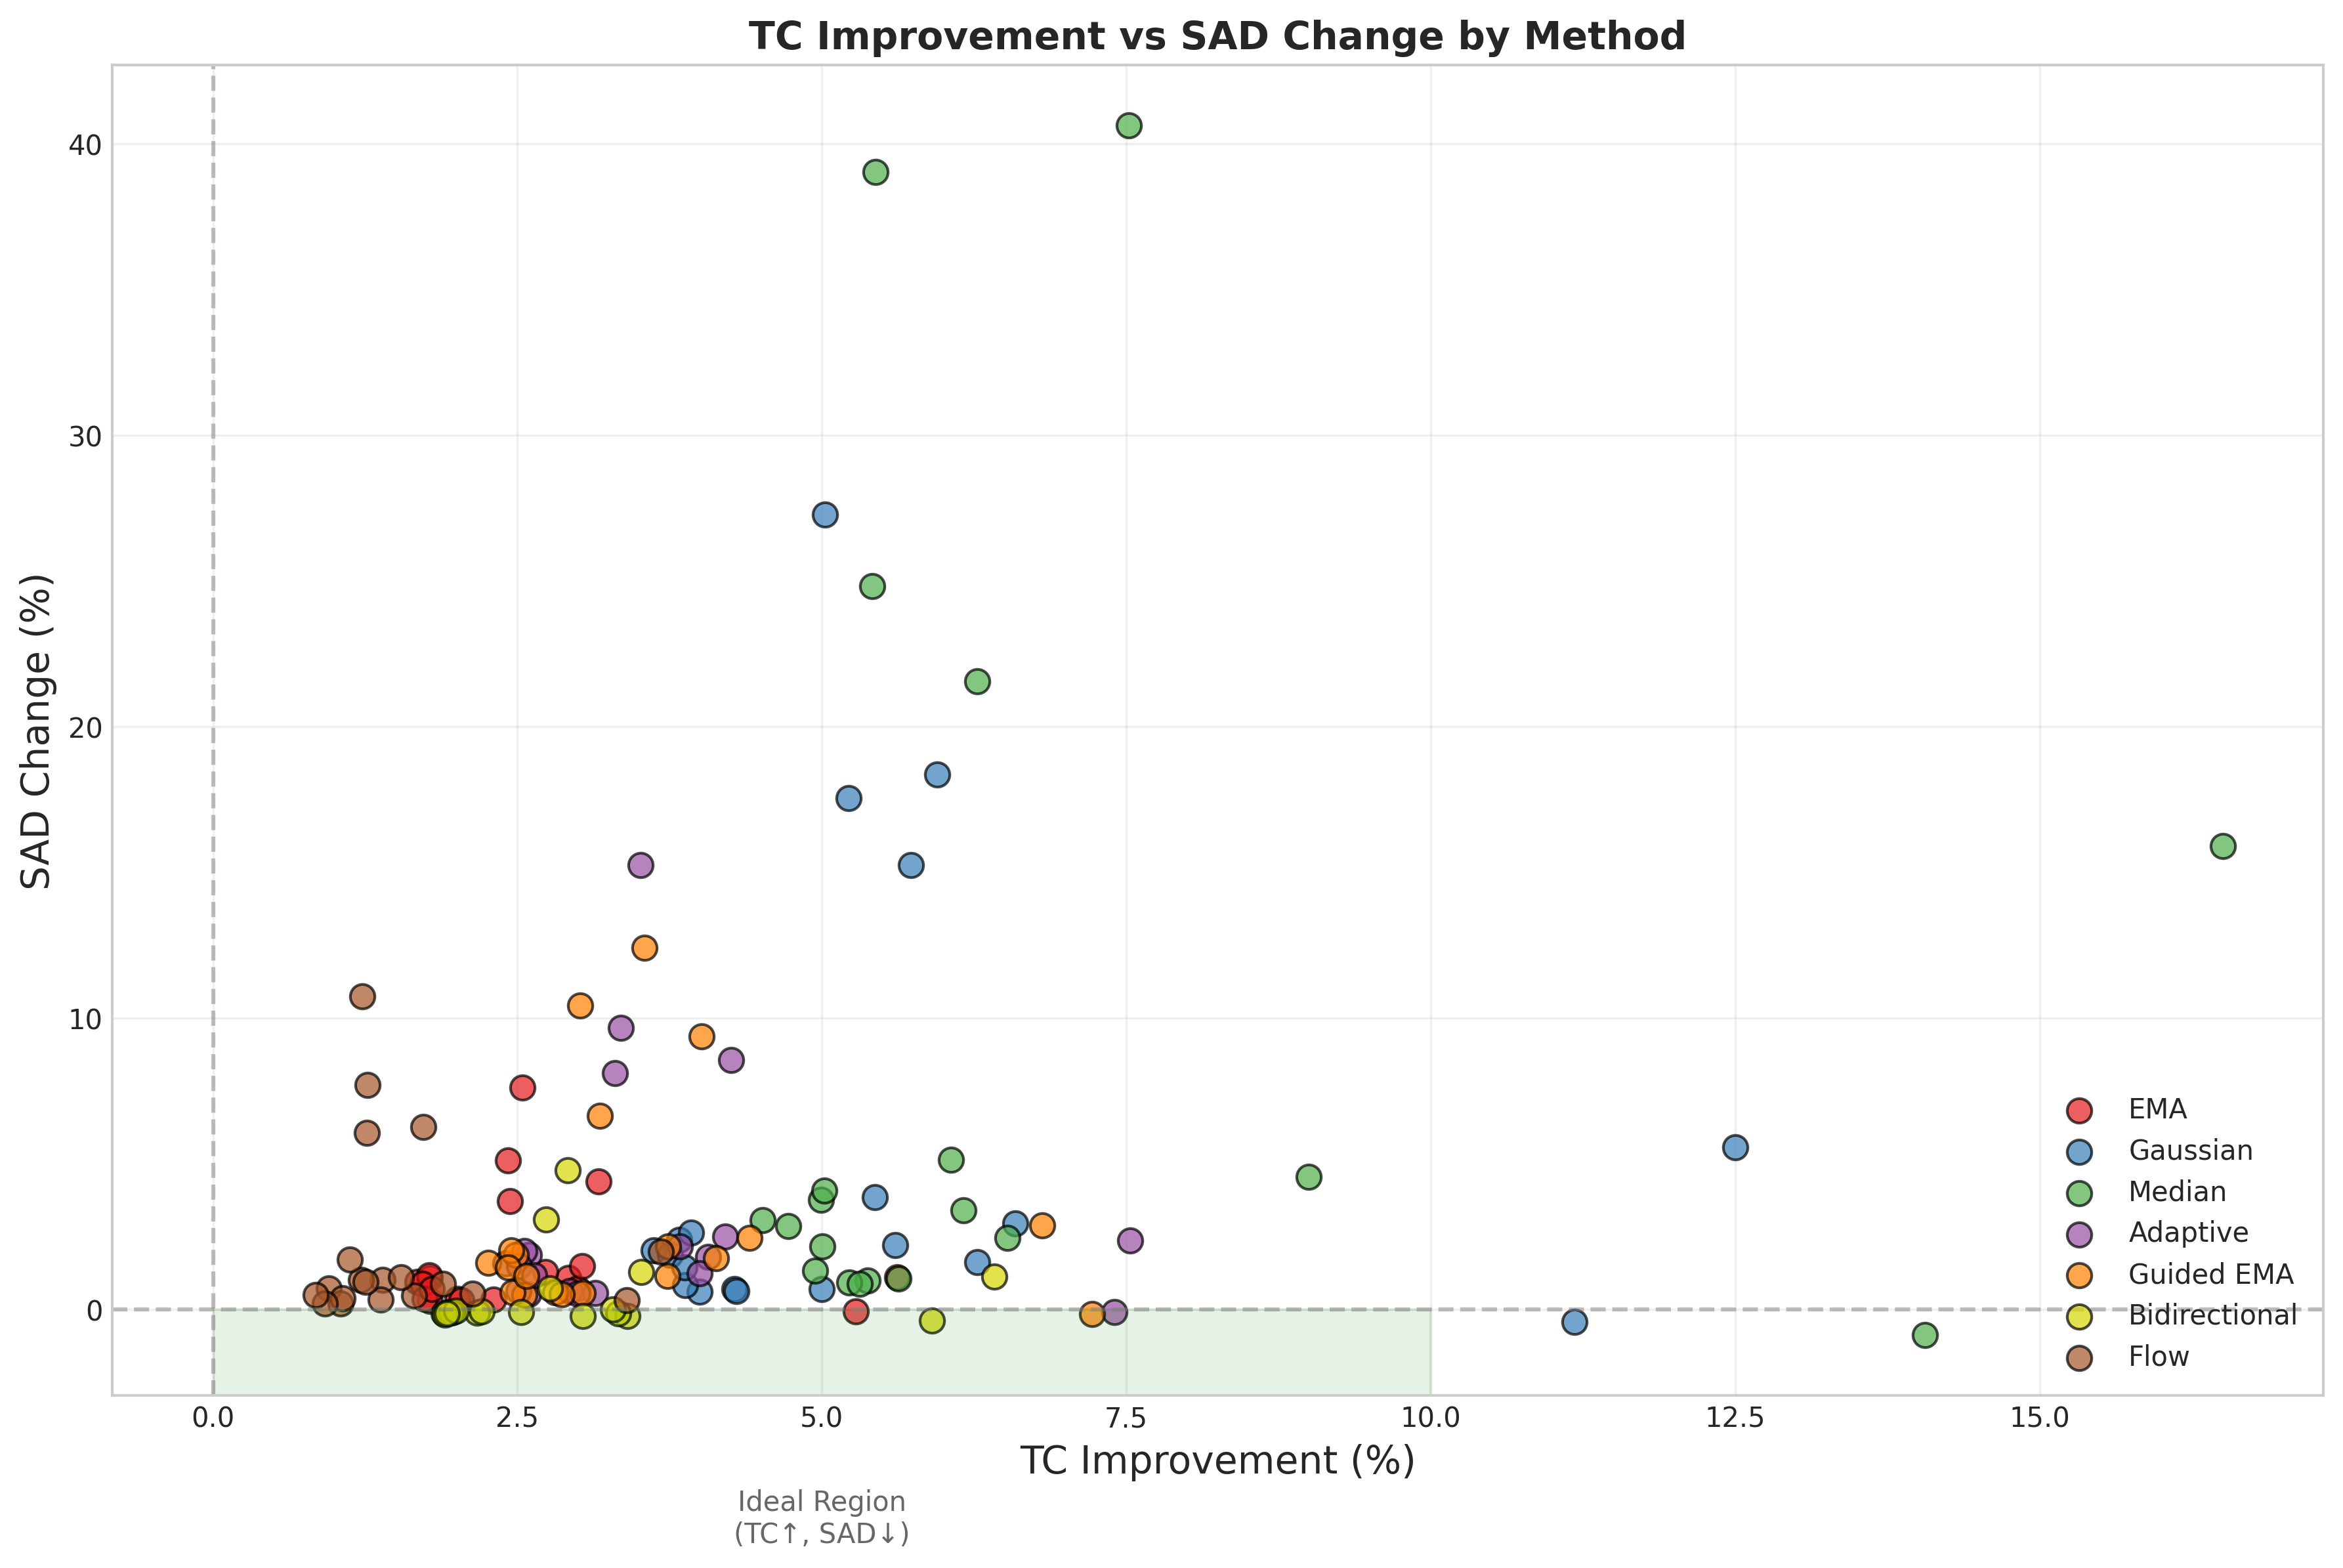
\includegraphics[width=\linewidth]{pic/figure1_tc_vs_sad_scatter.png}
      \vspace{0.1em}
      {\scriptsize  每个点代表一个视频的最佳结果}
      
    \column{0.4\textwidth}
      \begin{block}{解读}
        \begin{itemize}
          \setlength{\itemsep}{0.2em}
          \item 绿色区域：理想方向（TC↑，SAD↓）
          \item \textbf{Bidirectional}：最接近理想区域
          \item Median：TC 提升最大，但 SAD 增加显著
        \end{itemize}
      \end{block}
      
      \vspace{0.3em}
      \begin{block}{最佳参数}
        \scriptsize
        \begin{tabular}{ll}
          \toprule
          \textbf{方法} & \textbf{最佳参数} \\
          \midrule
          Median & window=7 \\
          Gaussian & sigma=2.0, window=7 \\
          \textbf{Bidirectional} & \textbf{alpha=0.7} \\
          \bottomrule
        \end{tabular}
      \end{block}
  \end{columns}
\end{frame}

\begin{frame}[t]{各方法性能分布箱线图}
  \scriptsize
  \linespread{0.98}\selectfont
  
  \begin{columns}[T,onlytextwidth]
    \column{0.7\textwidth}
      \centering
      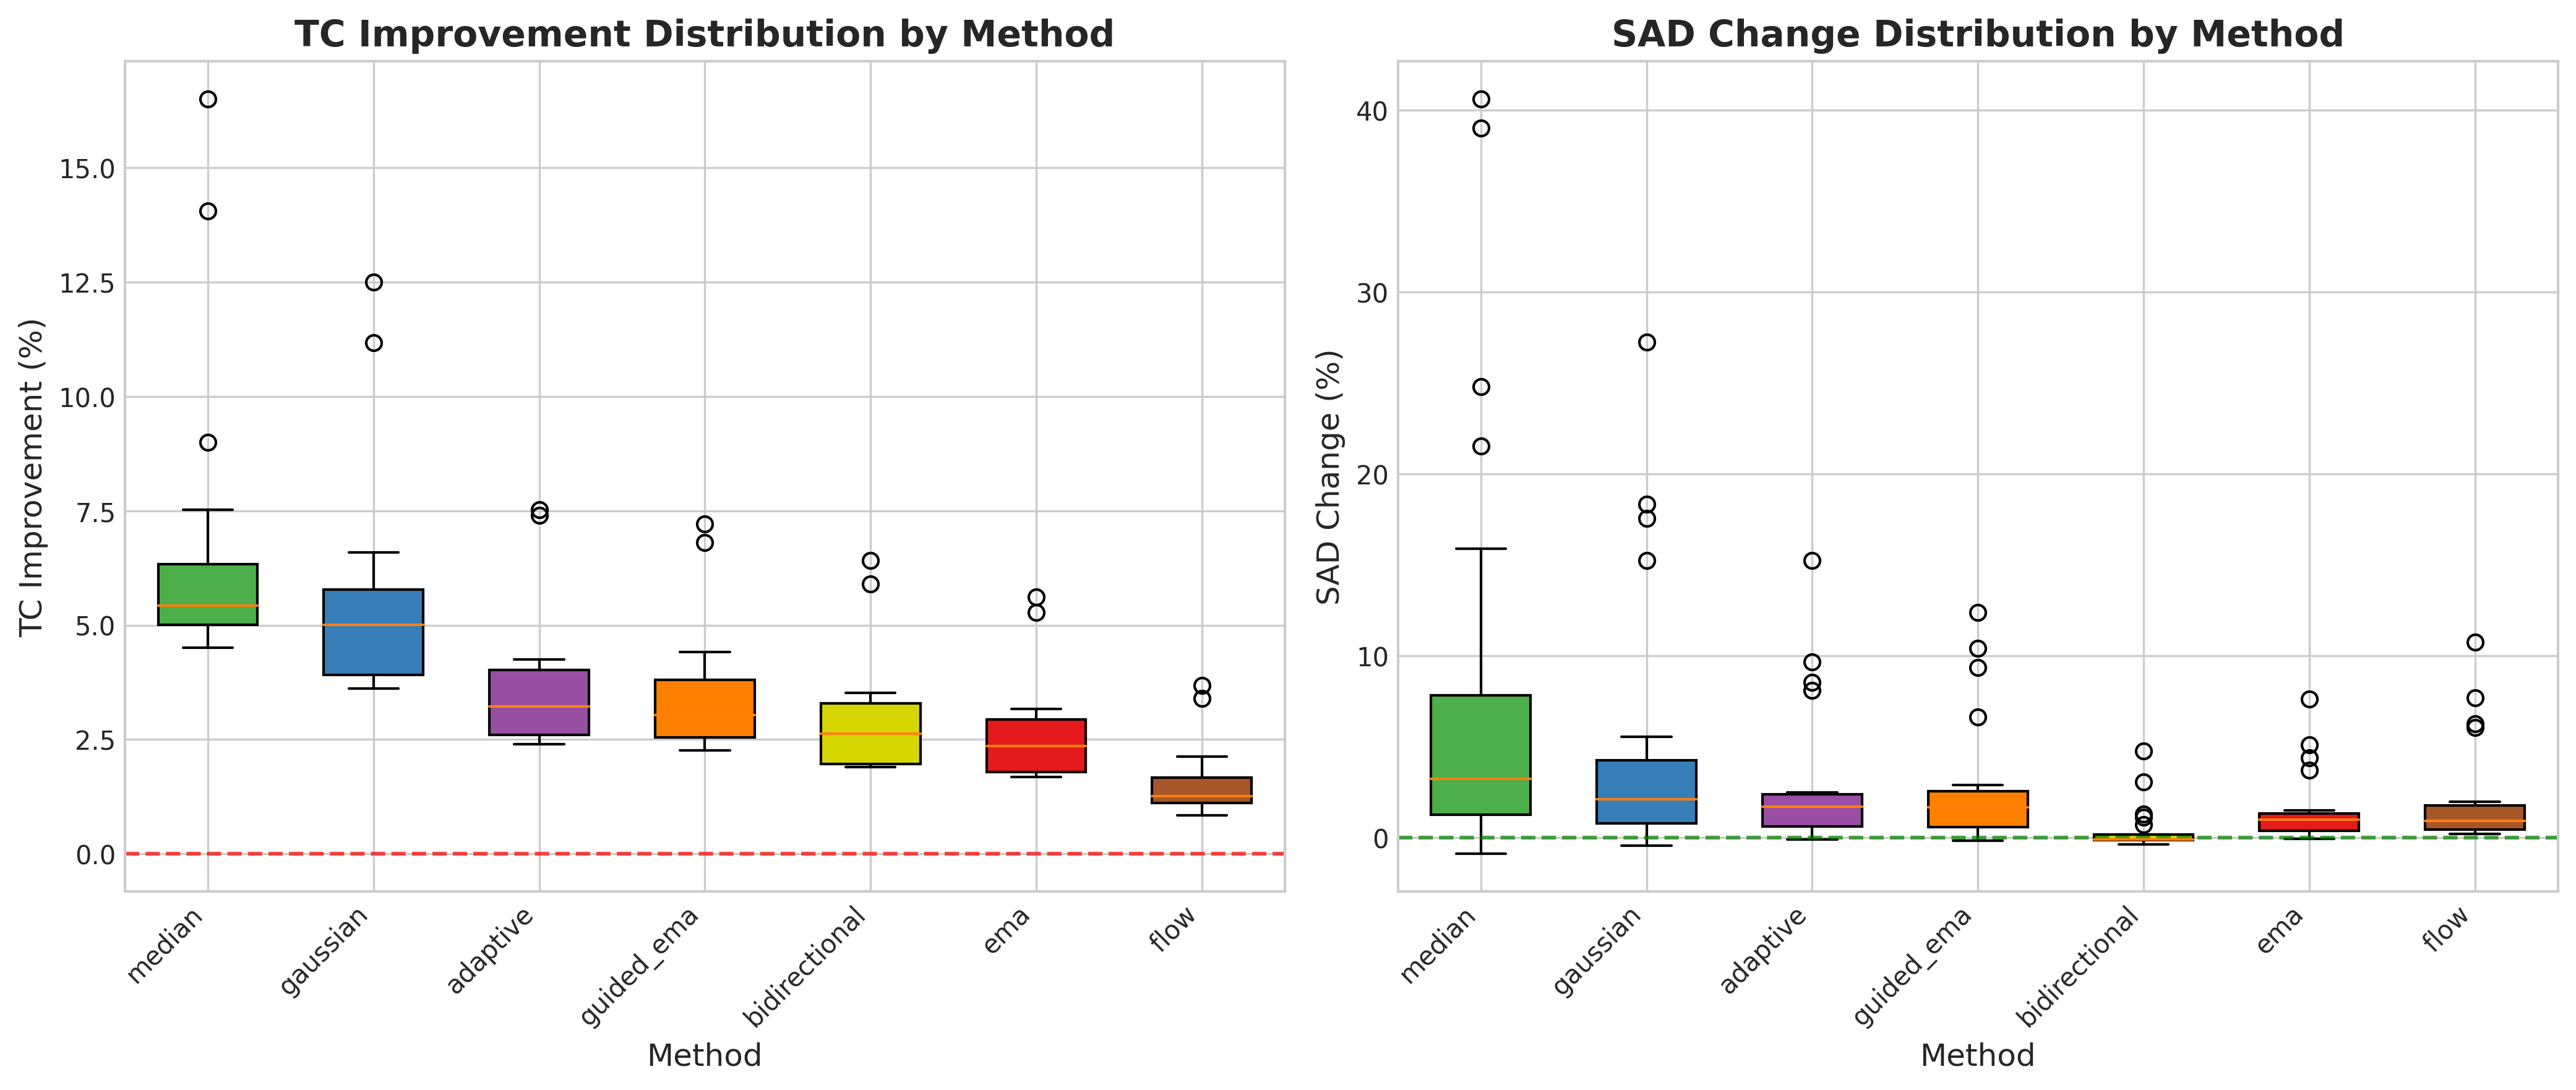
\includegraphics[width=\linewidth]{pic/figure2_method_comparison_boxplot.png}
      \vspace{0.1em}
      {\scriptsize 左：TC 提升分布 \quad | \quad 右：SAD 变化分布}
      
    \column{0.32\textwidth}
      \begin{block}{箱线图解读}
        \begin{itemize}
          \setlength{\itemsep}{0.2em}
          \item 箱体 = 四分位距（50\% 数据）
          \item 横线 = 中位数
          \item 圆形 = 异常值
        \end{itemize}
      \end{block}
      
      \vspace{0.3em}
      \begin{block}{关键观察}
        \begin{itemize}
          \setlength{\itemsep}{0.2em}
          \item \textbf{Bidirectional}：SAD 分布最集中，异常值最少
          \item \textbf{Median}：TC 提升高但波动大
          \item \textbf{Gaussian}：TC 提升分布较稳定
        \end{itemize}
      \end{block}
  \end{columns}
  
  \vspace{0.1em}
  \notestrip{nankai}{\scriptsize
  \textbf{结论：}Bidirectional 的 SAD 变化分布最集中，说明其精度表现\hilite{最稳定}，不同视频间差异最小。
  }
\end{frame}

\begin{frame}[t]{Bidirectional 平滑效果对比}
  \scriptsize
  \linespread{0.98}\selectfont
  
  \begin{columns}[T,onlytextwidth]
    \column{0.55\textwidth}
      \centering
      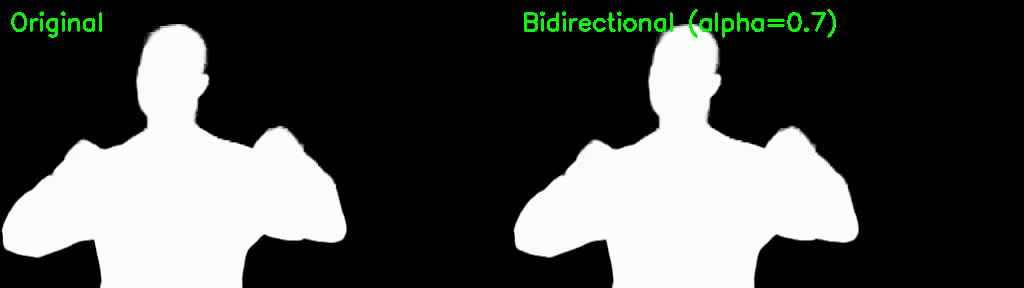
\includegraphics[width=0.98\linewidth]{pic/gif_frames/frame_0001.png}
      \vspace{0.1em}
      {\tiny 左：原始 alpha \quad | \quad 右：Bidirectional 平滑后}
      
      \vspace{0.2em}
      \href{run:pic/youtubematte_motion_0016_bidirectional_comparison_slow_hq.gif}{%
        \color{accentblue}{\underline{[Click] 点击播放动画效果 (GIF)}}%
      }
      
      \vspace{0.3em}
      \begin{block}{视觉效果}
        \begin{itemize}
          \setlength{\itemsep}{0.2em}
          \item 发丝细节\hilite{无明显模糊}
          \item 边缘抖动\hilite{明显减弱}
          \item 背景替换后\hilite{闪烁减少}
        \end{itemize}
      \end{block}
      
    \column{0.42\textwidth}
      \begin{block}{性能指标}
        \scriptsize
        \begin{tabular}{lcc}
          \toprule
          \textbf{指标} & \textbf{数值} & \textbf{评价} \\
          \midrule
          TC 提升 & 2.89\% & 提升 \\
          SAD 变化 & +0.44\% & 几乎无损 \\
          MSE 变化 & -0.12\% & 改善 \\
          \bottomrule
        \end{tabular}
      \end{block}
      
      \vspace{0.3em}
      \begin{block}{优劣分析}
        \scriptsize
        \begin{itemize}
          \setlength{\itemsep}{0.1em}
          \item \textbf{优点：}精度几乎无损，发丝细节保留完整
          \item \textbf{缺点：}TC 提升幅度相对较小
        \end{itemize}
      \end{block}
  \end{columns}
  
  \vspace{0.2em}
  \notestrip{softgreen}{\scriptsize
  \textbf{结论：}Bidirectional 在\hilite{保持视觉质量的同时}实现时序一致性提升，是精度无损场景的最佳选择。
  }
\end{frame}

\begin{frame}[t]{Median 平滑效果对比}
  \scriptsize
  \linespread{0.98}\selectfont
  
  \begin{columns}[T,onlytextwidth]
    \column{0.55\textwidth}
      \centering
      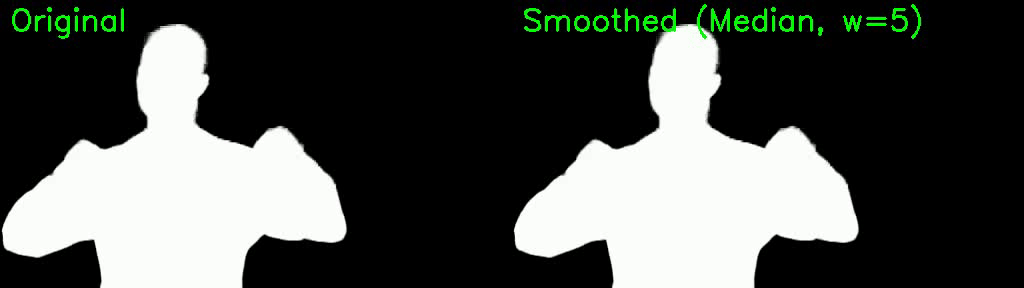
\includegraphics[width=0.98\linewidth]{pic/median_frames/median_frame_0001.png}
      \vspace{0.1em}
      {\tiny 左：原始 alpha \quad | \quad 右：Median 平滑后}
      
      \vspace{0.2em}
      \href{run:pic/youtubematte_motion_0016_comparison_slow_hq.gif}{%
        \color{accentblue}{\underline{[Click] 点击播放动画效果 (GIF)}}%
      }
      
      \vspace{0.3em}
      \begin{block}{视觉效果}
        \begin{itemize}
          \setlength{\itemsep}{0.2em}
          \item 发丝细节\hilite{明显模糊}
          \item 边缘抖动\hilite{减少但细节丢失}
          \item 背景替换后\hilite{毛边明显}
        \end{itemize}
      \end{block}
      
    \column{0.42\textwidth}
      \begin{block}{性能指标}
        \scriptsize
        \begin{tabular}{lcc}
          \toprule
          \textbf{指标} & \textbf{数值} & \textbf{评价} \\
          \midrule
          TC 提升 & 6.68\% & 提升最大 \\
          SAD 变化 & +8.88\% & 恶化严重 \\
          MSE 变化 & +23.91\% & 恶化严重 \\
          \bottomrule
        \end{tabular}
      \end{block}
      
      \vspace{0.3em}
      \begin{block}{优劣分析}
        \scriptsize
        \begin{itemize}
          \setlength{\itemsep}{0.1em}
          \item \textbf{优点：}TC 提升最大（6.68\%），时序稳定性最好
          \item \textbf{缺点：}发丝模糊严重，视觉损失不可接受
        \end{itemize}
      \end{block}
  \end{columns}
  
  \vspace{0.2em}
  \notestrip{softorange}{\scriptsize
  \textbf{结论：}Median 数值最优但\hilite{视觉损失严重}，不适合需要精细边缘的实际应用。
  }
\end{frame}


\begin{frame}[t]{Gaussian 平滑效果对比}
  \scriptsize
  \linespread{0.98}\selectfont
  
  \begin{columns}[T,onlytextwidth]
    \column{0.55\textwidth}
      \centering
      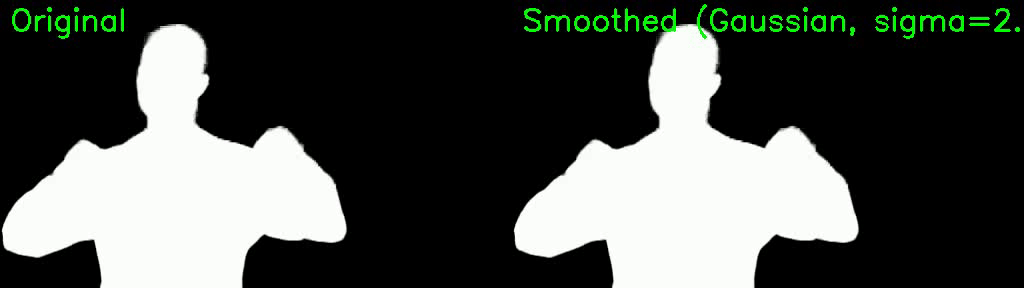
\includegraphics[width=0.98\linewidth]{pic/gaussian_frames/gaussian_frame_0001.png}
      \vspace{0.1em}
      {\tiny 左：原始 alpha \quad | \quad 右：Gaussian 平滑后 (sigma=2.0)}
      
      \vspace{0.2em}
      \href{run:pic/youtubematte_motion_0016_gaussian_comparison_slow_hq.gif}{%
        \color{accentblue}{\underline{[Click] 点击播放动画效果 (GIF)}}%
      }
      
      \vspace{0.3em}
      \begin{block}{视觉效果}
        \begin{itemize}
          \setlength{\itemsep}{0.2em}
          \item 发丝细节\hilite{轻微模糊}
          \item 边缘抖动\hilite{明显减少}
          \item 整体\hilite{平衡性较好}
        \end{itemize}
      \end{block}
      
    \column{0.42\textwidth}
      \begin{block}{性能指标}
        \scriptsize
        \begin{tabular}{lcc}
          \toprule
          \textbf{指标} & \textbf{数值} & \textbf{评价} \\
          \midrule
          TC 提升 & 4.0\% & 提升显著 \\
          SAD 变化 & +2.4\% & 轻微恶化 \\
          MSE 变化 & +3.0\% & 轻微恶化 \\
          \bottomrule
        \end{tabular}
      \end{block}
      
      \vspace{0.3em}
      \begin{block}{优劣分析}
        \scriptsize
        \begin{itemize}
          \setlength{\itemsep}{0.1em}
          \item \textbf{优点：}TC 提升显著（4.0\%），是 TC 和精度的最佳平衡点
          \item \textbf{缺点：}发丝有轻微模糊，精度略有下降
        \end{itemize}
      \end{block}
  \end{columns}
  
  \vspace{0.2em}
  \notestrip{accentblue}{\scriptsize
  \textbf{建议：}追求平衡可选 Gaussian (sigma=2.0, window=5)；追求精度无损可选 Bidirectional (alpha=0.7)。
  }
\end{frame}


\begin{frame}[t]{两个数据集上的性能对比}
  \scriptsize
  \linespread{0.98}\selectfont
  
  \begin{columns}[T,onlytextwidth]
    \column{0.7\textwidth}
      \centering
      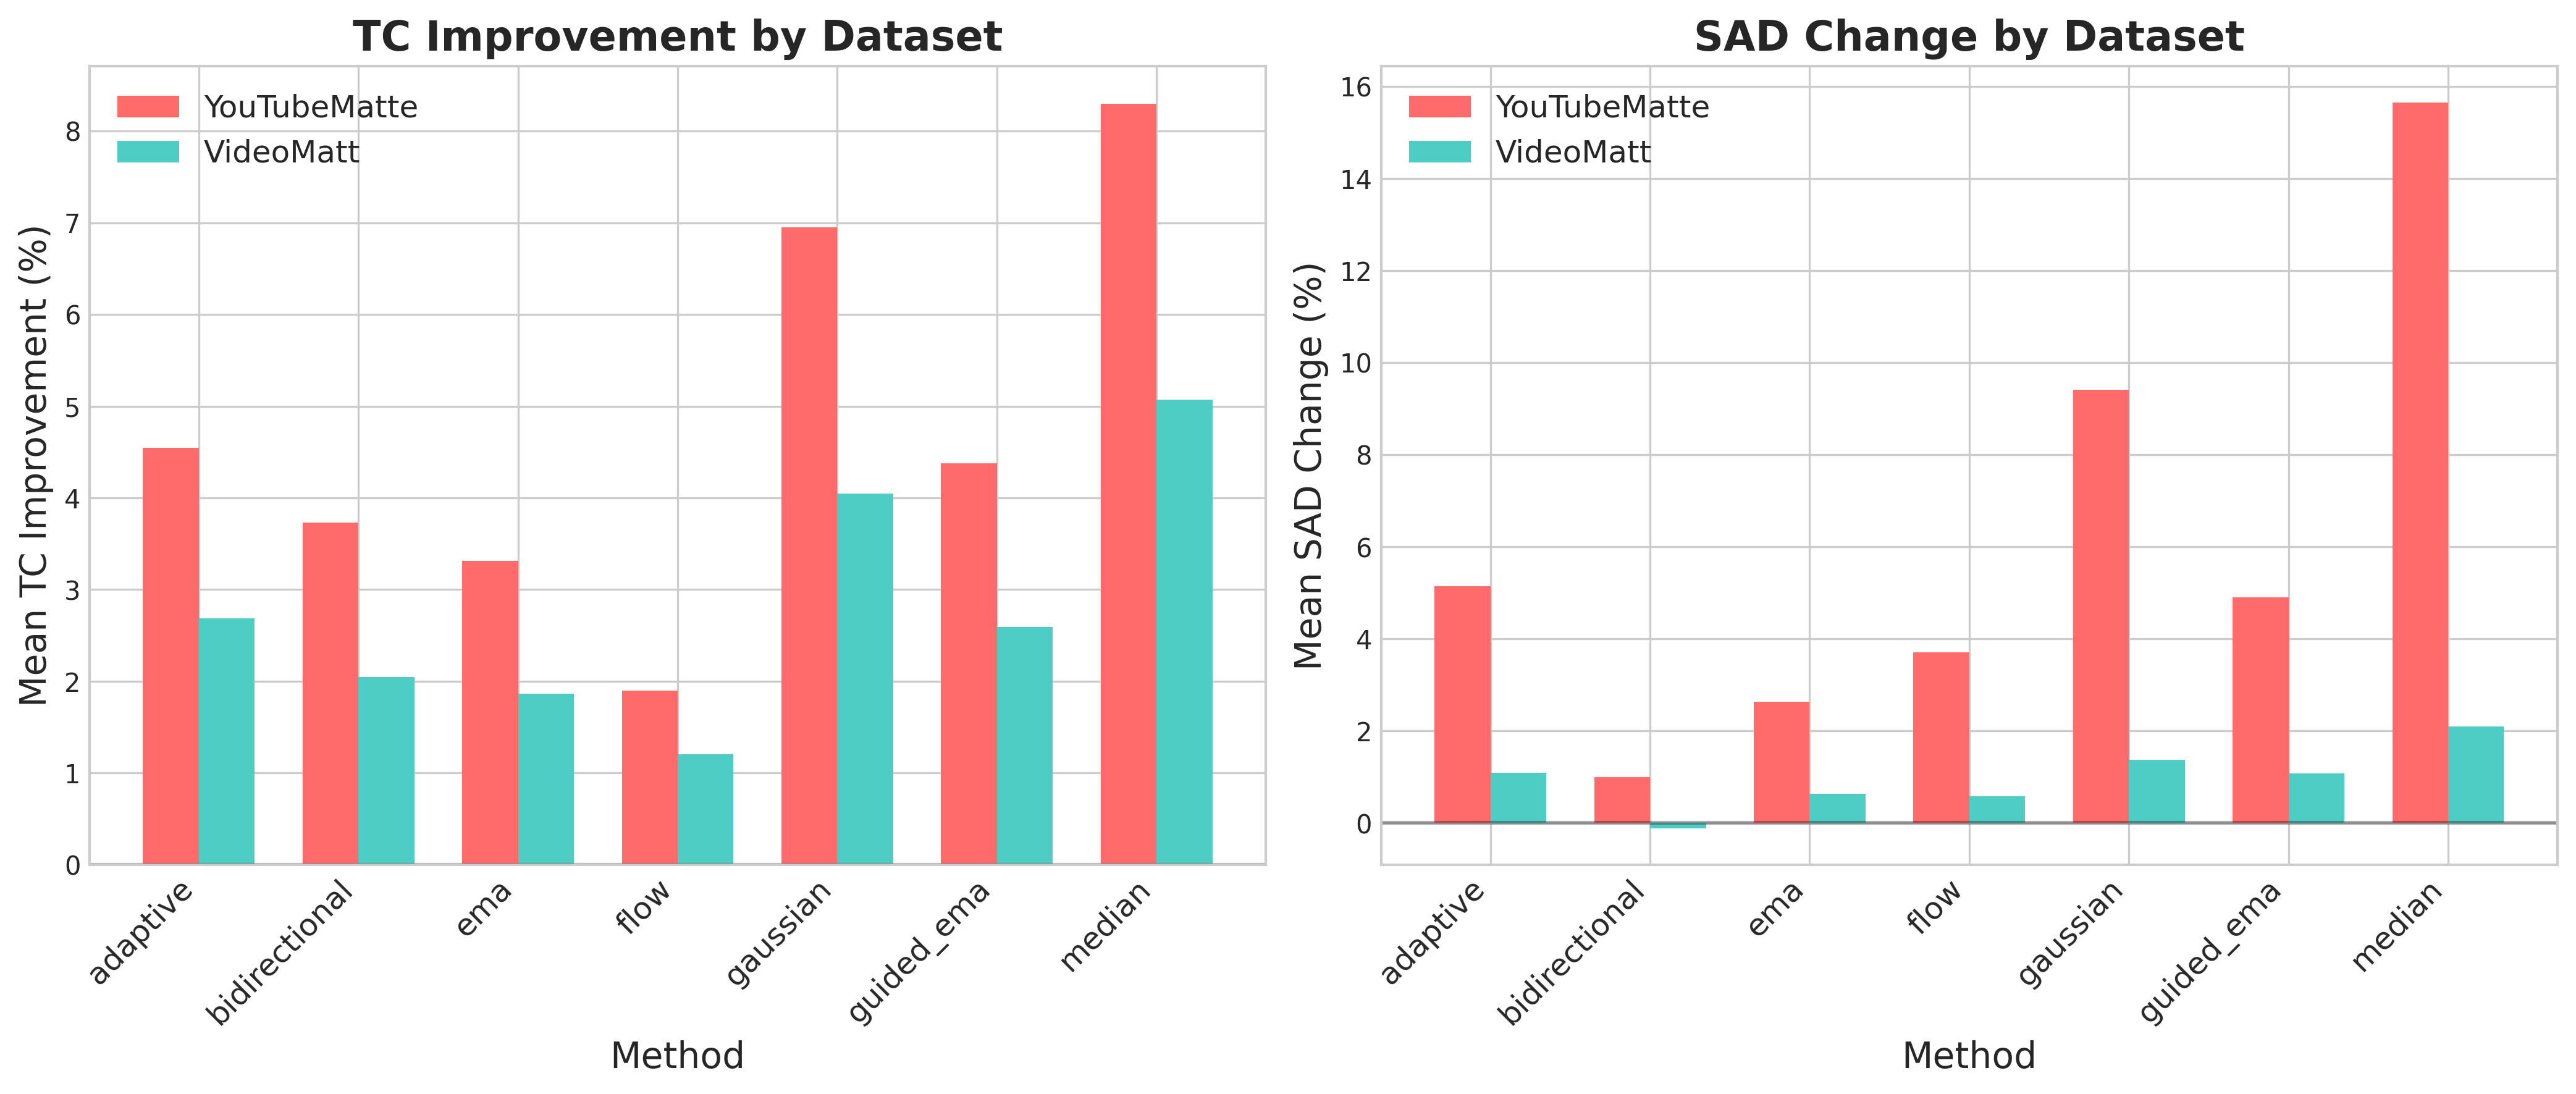
\includegraphics[width=0.98\linewidth]{pic/figure3_dataset_comparison.png}
      \vspace{0.1em}
      {\scriptsize 左：TC 提升对比 \quad | \quad 右：SAD 变化对比}
      
    \column{0.32\textwidth}
      \begin{block}{关键观察}
        \begin{itemize}
          \setlength{\itemsep}{0.2em}
          \item YouTubeMatte 上效果\hilite{普遍更好}
          \item VideoMatt 更具挑战性
          \item \textbf{Bidirectional} 表现\hilite{最稳定}
        \end{itemize}
      \end{block}
      
      \vspace{0.5em}
      \begin{block}{差异分析}
        \scriptsize
        VideoMatt 包含更多\hilite{复杂运动}和\hilite{精细结构}，平滑难度更高。
      \end{block}
    \end{columns}
   \vspace{0.1em}
  \notestrip{accentblue}{\scriptsize
  \textbf{结论：}Bidirectional 在两个数据集上表现最稳定，适合不同场景的视频抠图任务。
  }
\end{frame}

\begin{frame}[t]{Gaussian 参数敏感性分析}
  \vspace{-0.5cm}
  \scriptsize
  \linespread{0.98}\selectfont
  
  \begin{columns}[T,onlytextwidth]
    \column{0.65\textwidth}
      \centering
      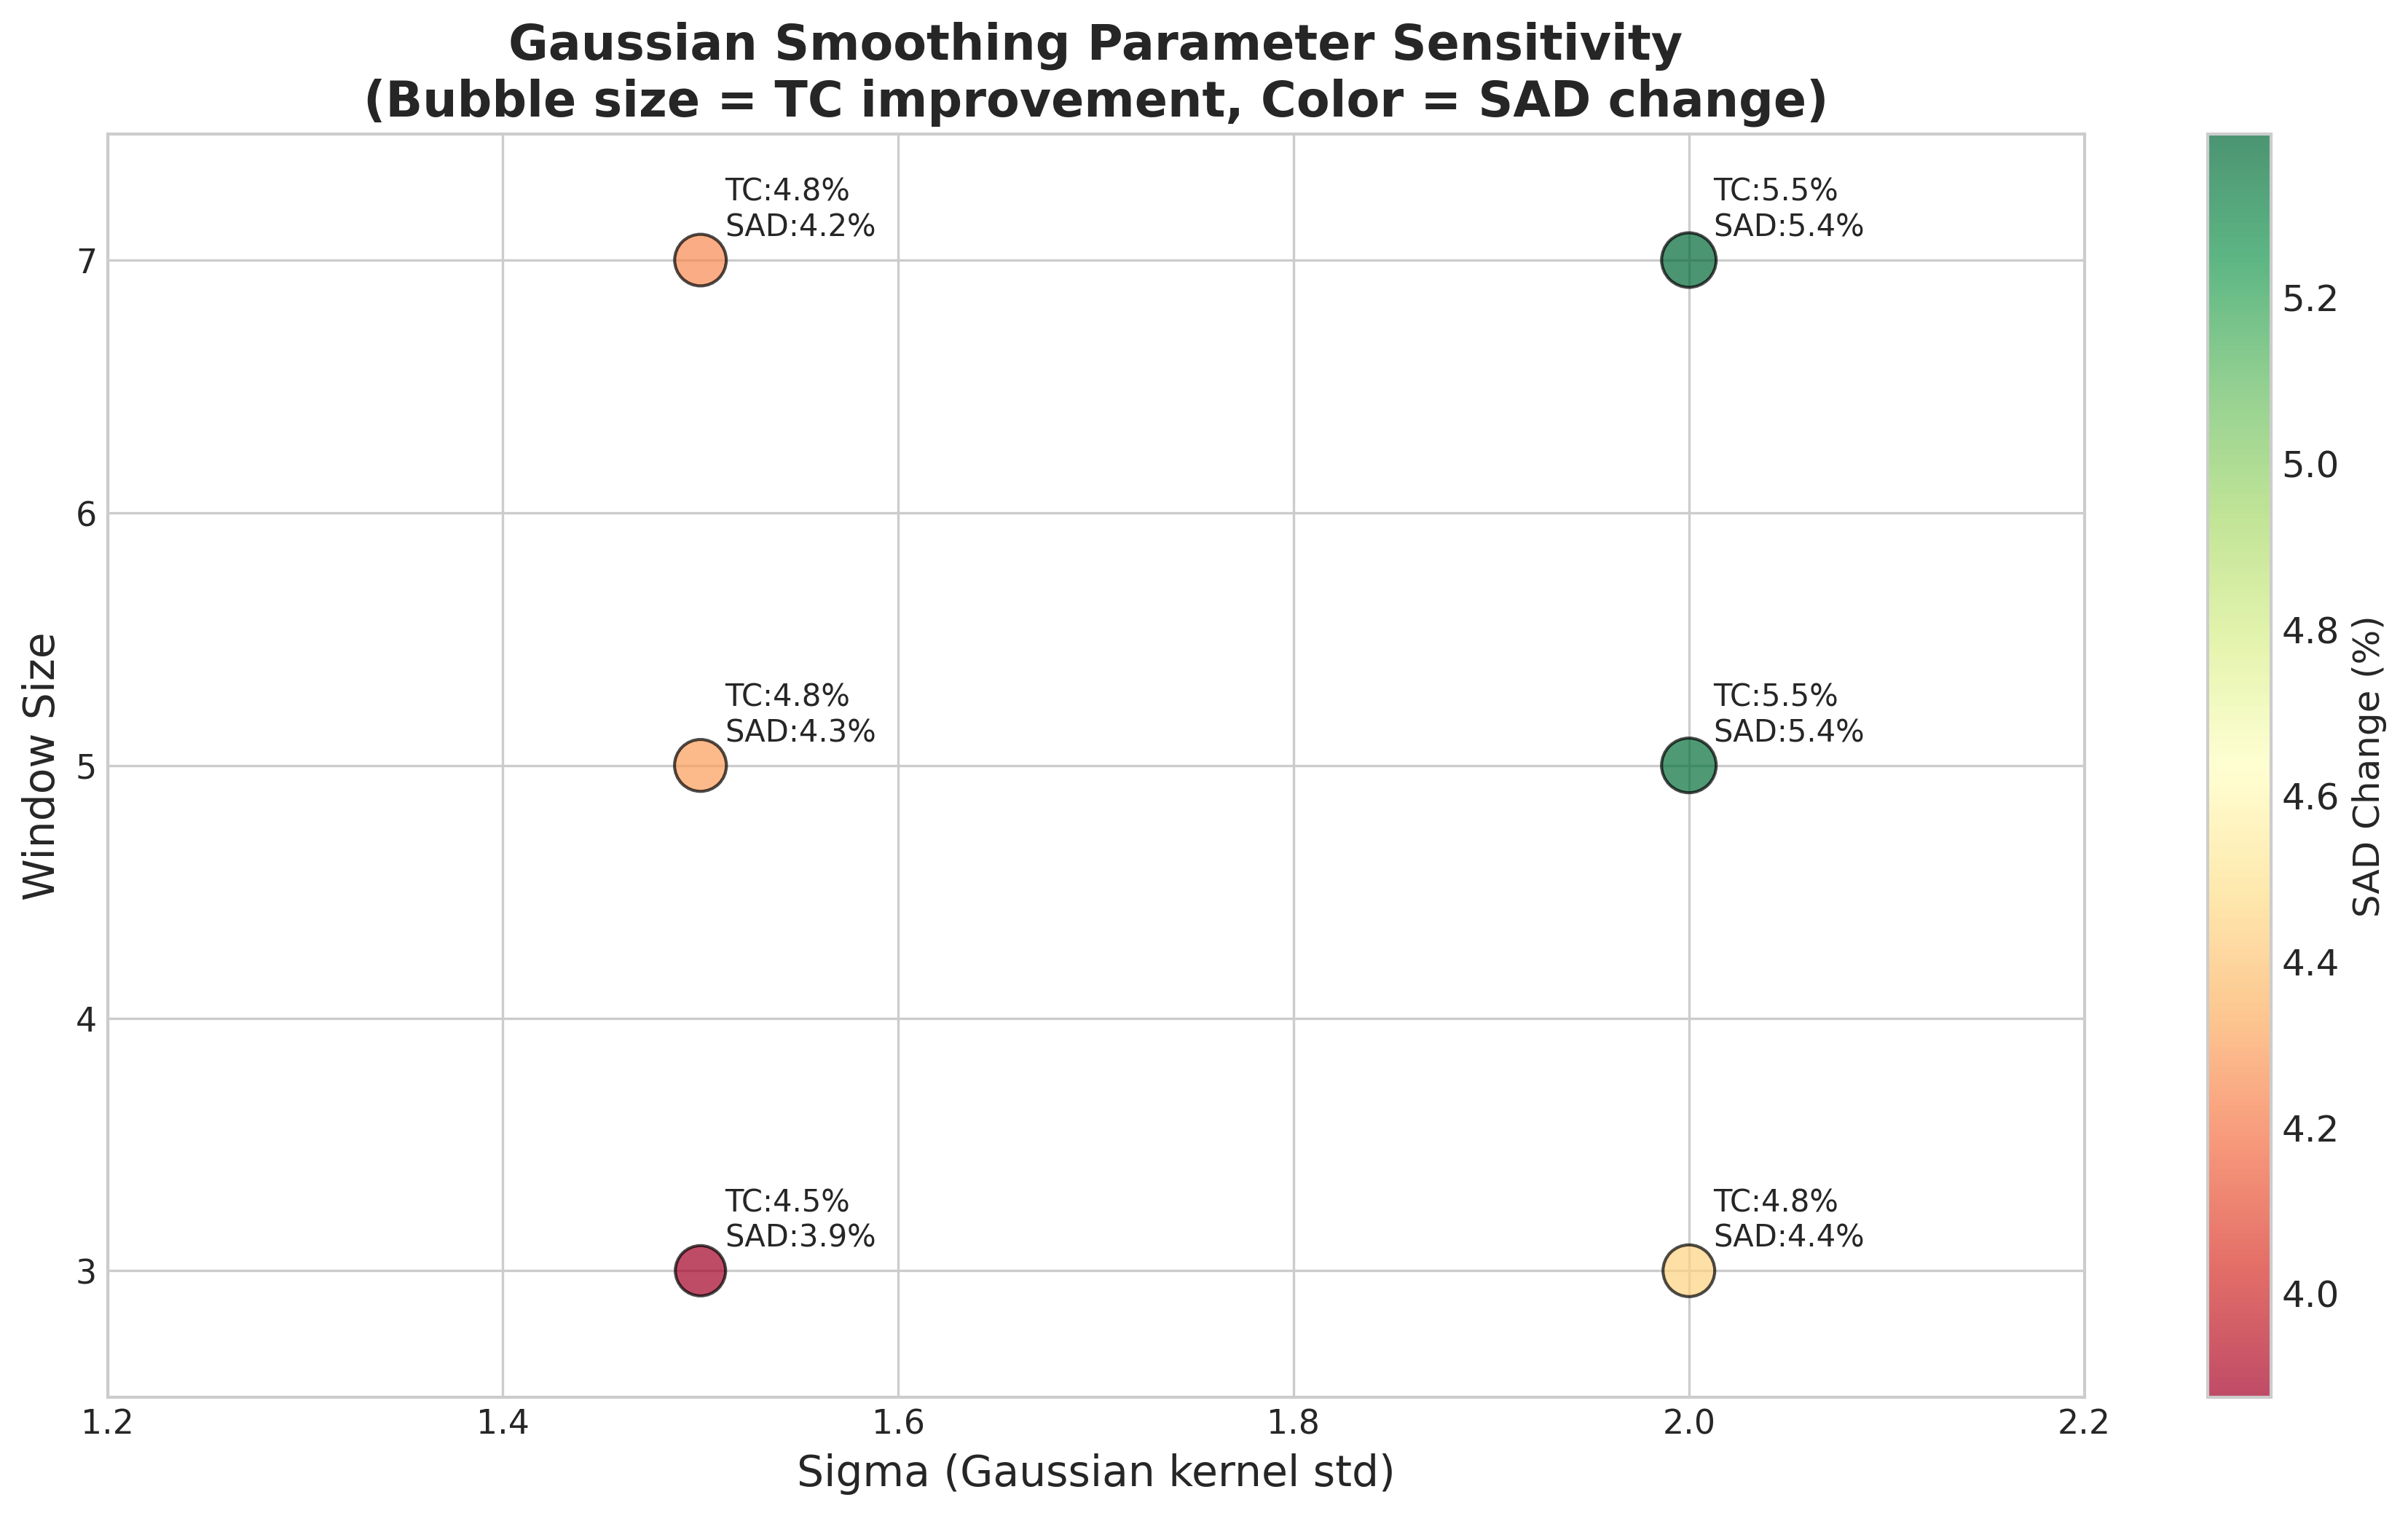
\includegraphics[width=0.98\linewidth]{pic/figure4_gaussian_parameter_sensitivity.png}
      \vspace{0.1em}
      {\scriptsize 气泡大小 = TC 提升，颜色 = SAD 变化}
      
    \column{0.32\textwidth}
      \begin{block}{参数趋势}
        \begin{itemize}
          \setlength{\itemsep}{0.2em}
          \item 增大 sigma → TC 提升增加
          \item 增大 sigma → SAD 恶化加剧
          \item 增大窗口 → 效果饱和
        \end{itemize}
      \end{block}
      
      \vspace{0.3em}
      \begin{block}{推荐参数}
        \centering
        \metricchip{softgreen}{sigma=2.0}{window=5} \\
        \vspace{0.1em}
        {\scriptsize TC 提升: 4.0\%, SAD 增加: 2.4\%}
      \end{block}
  \end{columns}
  
  \vspace{0.1em}
  \notestrip{accentblue}{\scriptsize
  \textbf{建议：}追求平衡可选 Gaussian；追求精度无损可选 Bidirectional。
  }
\end{frame}

\begin{frame}[t]{综合性能雷达图}
  \vspace{-0.5cm}
  \scriptsize
  \linespread{0.98}\selectfont
  
  \begin{columns}[T,onlytextwidth]
    \column{0.60\textwidth}
      \centering
      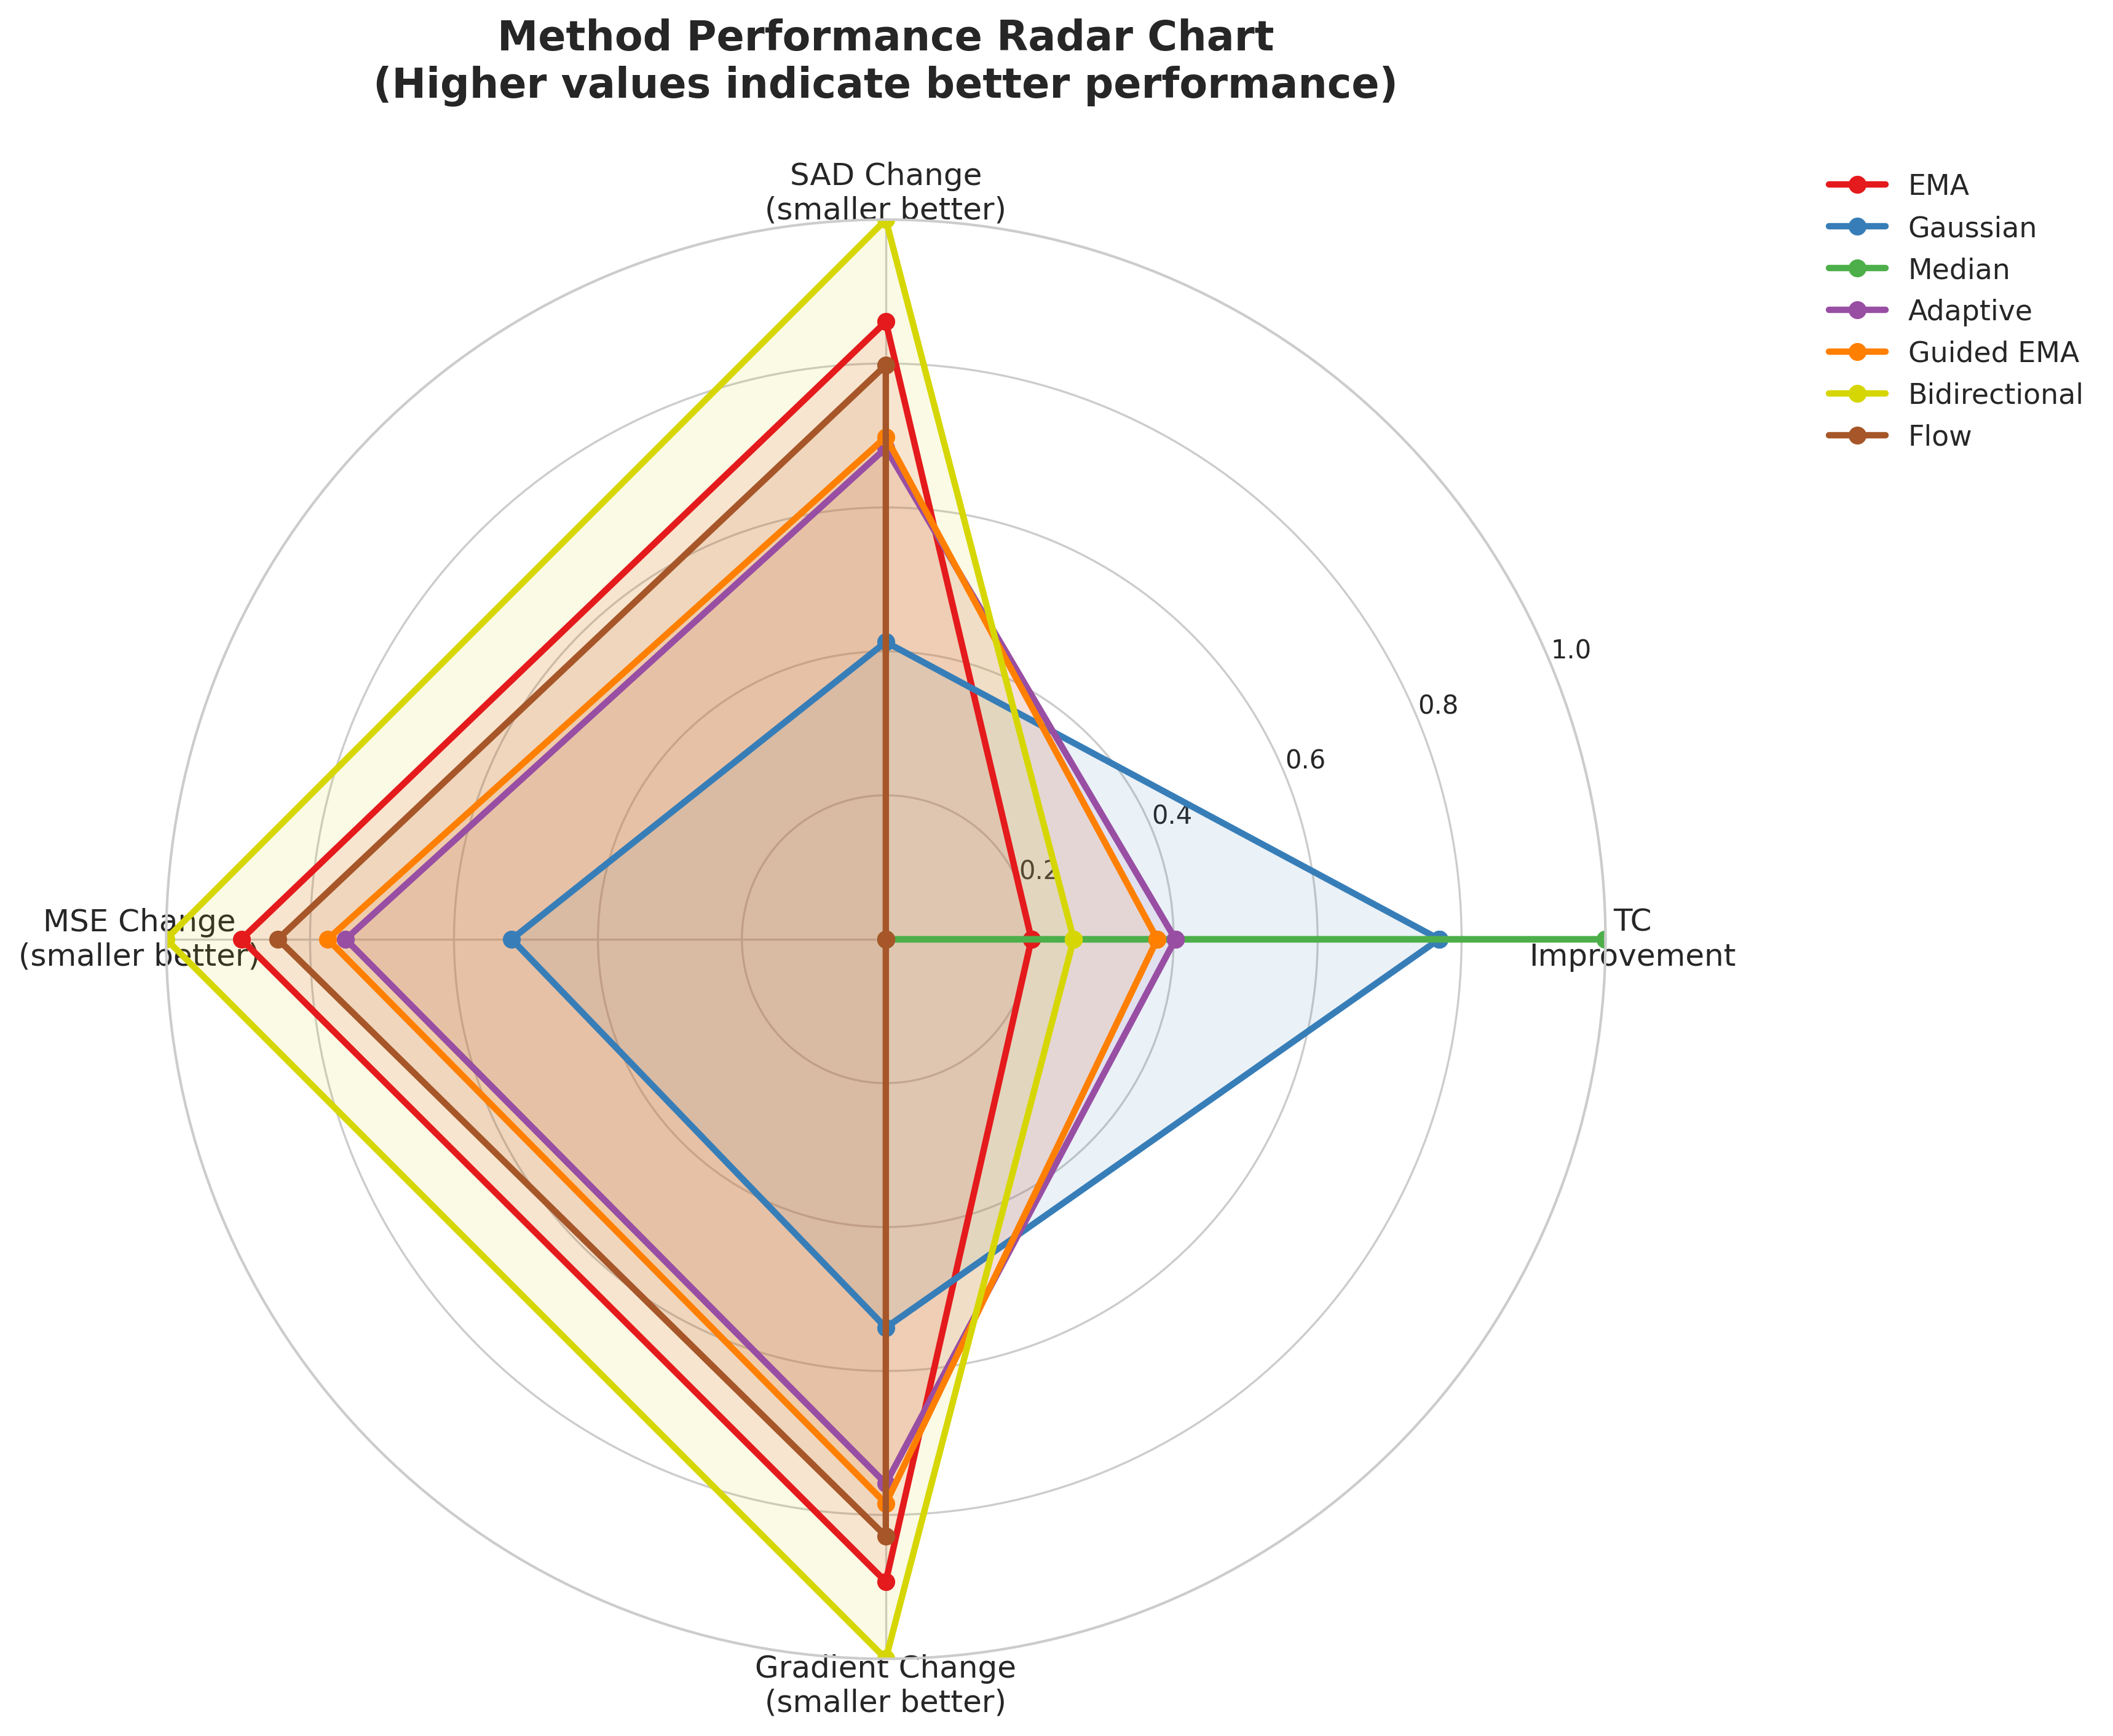
\includegraphics[width=0.95\linewidth]{pic/figure5_radar_chart.png}
      
    \column{0.32\textwidth}
      \begin{block}{解读}
        \begin{itemize}
          \setlength{\itemsep}{0.2em}
          \item 雷达图中 SAD/MSE/Gradient 已反向归一化，\hilite{值越大 = 性能越好}。
          \item \textbf{Bidirectional} 最均衡
          \item Median 偏科严重
        \end{itemize}
      \end{block}
      
      \vspace{0.3em}
      \begin{block}{总结}
        \centering
        \textbf{Bidirectional (alpha=0.7)} \\
        \vspace{0.1em}
        → 雷达图面积最大 \\
        → 推荐为默认平滑策略
      \end{block}
  \end{columns}
  
  
\end{frame}

\begin{frame}[t]{视频换背景 Demo}
  \scriptsize
  \linespread{0.98}\selectfont
  
  \begin{columns}[T,onlytextwidth]
    \column{0.48\textwidth}
      \begin{block}{平滑后 alpha 对比}
        \centering
        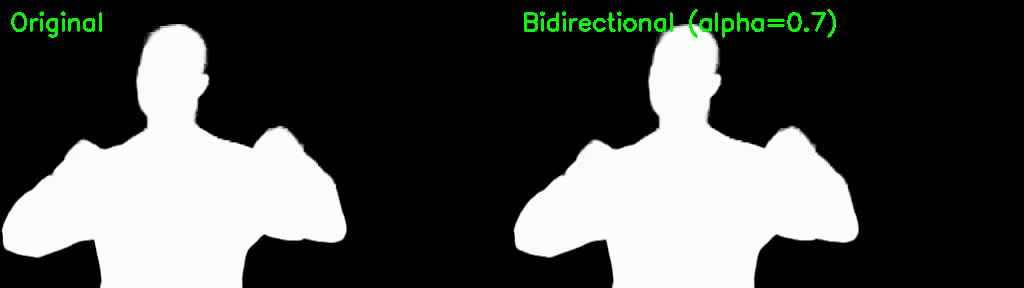
\includegraphics[width=0.95\linewidth]{pic/gif_frames/frame_0001.png}
        \vspace{0.1em}
        {\scriptsize 左：原始 \quad | \quad 右：Bidirectional 平滑后}
        
        \vspace{0.2em}
        \href{run:pic/youtubematte_motion_0016_bidirectional_slow_hq.gif}{%
          \color{accentblue}{\underline{[Click] 播放动画效果 (GIF)}}%
        }
      \end{block}
      
    \column{0.48\textwidth}
      \begin{block}{换背景效果}
        \centering
        
\includegraphics[width=0.35\linewidth]{pic/background.jpg}
        \vspace{0.1em}
        \\
        {\scriptsize 平滑后 alpha → RGBA → 背景替换}
        
        \vspace{0.2em}
        \href{run:pic/youtubematte_motion_0016_bidirectional_composer.mp4}{%
          \color{accentblue}{\underline{[Click] 播放换背景动画 (mp4)}}%
        }
      \end{block}
  \end{columns}
  
  \vspace{0.2em}
  \begin{block}{接口说明}
    \scriptsize
    \textbf{输入：}图像主线首帧 alpha / mask
    \textbf{处理：}MatAnyone2 + Bidirectional 时序平滑 (alpha=0.7)
    \textbf{输出：}逐帧稳定 alpha + 换背景合成视频
  \end{block}
  
  \vspace{0.1em}
  \notestrip{softgreen}{\scriptsize
  \textbf{效果：}Bidirectional 平滑后，背景替换视频的\hilite{边界闪烁明显减少}，同时\hilite{发丝细节保持清晰}。
  }
\end{frame} 引入，
%    继承主文件导言区的全部宏 / 配色 / 字体，无需自带 \documentclass 或 \begin{document}。
%  · 直接在下面增删 \begin{frame}[t]{标题} ... \end{frame} 即可。
%  · 可复用样式：
%       \hilite{} \tcard{} \ccard{} \notestrip{} \metricchip{} \mpill[] \pill[]
%     可选 accent：nankai、accentblue、softgreen、softorange、softgray、deepred
% ============================================================================

\section{视频与应用}

\begin{frame}[t]{视频抠图与时序平滑}
  \scriptsize
  \linespread{0.98}\selectfont
  
  \begin{columns}[T,onlytextwidth]
    \column{0.48\textwidth}
      \begin{block}{问题：视频 alpha 抖动}
        \begin{itemize}
          \setlength{\itemsep}{0.2em}
          \item MatAnyone2~{\scriptsize[7]} 逐帧推理时，alpha 存在帧间\hilite{抖动与边界闪烁}；
          \item 直接替换背景会放大这些不稳定，导致视觉不自然；
          \item 需要一种\hilite{保持细节}的时序平滑策略。
        \end{itemize}
      \end{block}
      
      \vspace{0.2em}
      \begin{block}{解决方案：边界带时序平滑}
        \centering
        \resizebox{0.95\linewidth}{!}{%
        \begin{tikzpicture}[
          >={Latex[length=2.5mm,width=2mm]},
          node distance=3mm,
          every node/.style={font=\scriptsize},
          vcard/.style={rounded corners=2pt, line width=0.8pt, align=center, inner sep=3pt},
          vblue/.style={vcard, draw=accentblue!82!black, fill=accentblue!12},
          vpurple/.style={vcard, draw=nankai!88!black, fill=nankai!12},
          vgreen/.style={vcard, draw=softgreen!72!black, fill=softgreen!14},
          varrow/.style={-{Latex[length=2.5mm,width=2mm]}, line width=1.2pt, draw=nankai!80!black}
        ]
          \node[vblue] (input) {\textbf{输入}\\alpha video};
          \node[vpurple, right=of input] (detect) {\textbf{边界检测}\\$0.05<\alpha<0.95$};
          \node[vgreen, right=of detect] (smooth) {\textbf{时序平滑}\\EMA / Bidirectional};
          \node[vblue, right=of smooth] (output) {\textbf{输出}\\稳定 alpha};
          \draw[varrow] (input) -- (detect);
          \draw[varrow] (detect) -- (smooth);
          \draw[varrow] (smooth) -- (output);
        \end{tikzpicture}}
        
        \vspace{0.2em}
        \scriptsize
        仅在边界区域（$\alpha\in[0.05,0.95]$）施加平滑，\hilite{保护前景核区与背景}，避免过度模糊。
      \end{block}
      
    \column{0.48\textwidth}
      \begin{block}{7 种平滑策略对比}
        \centering
        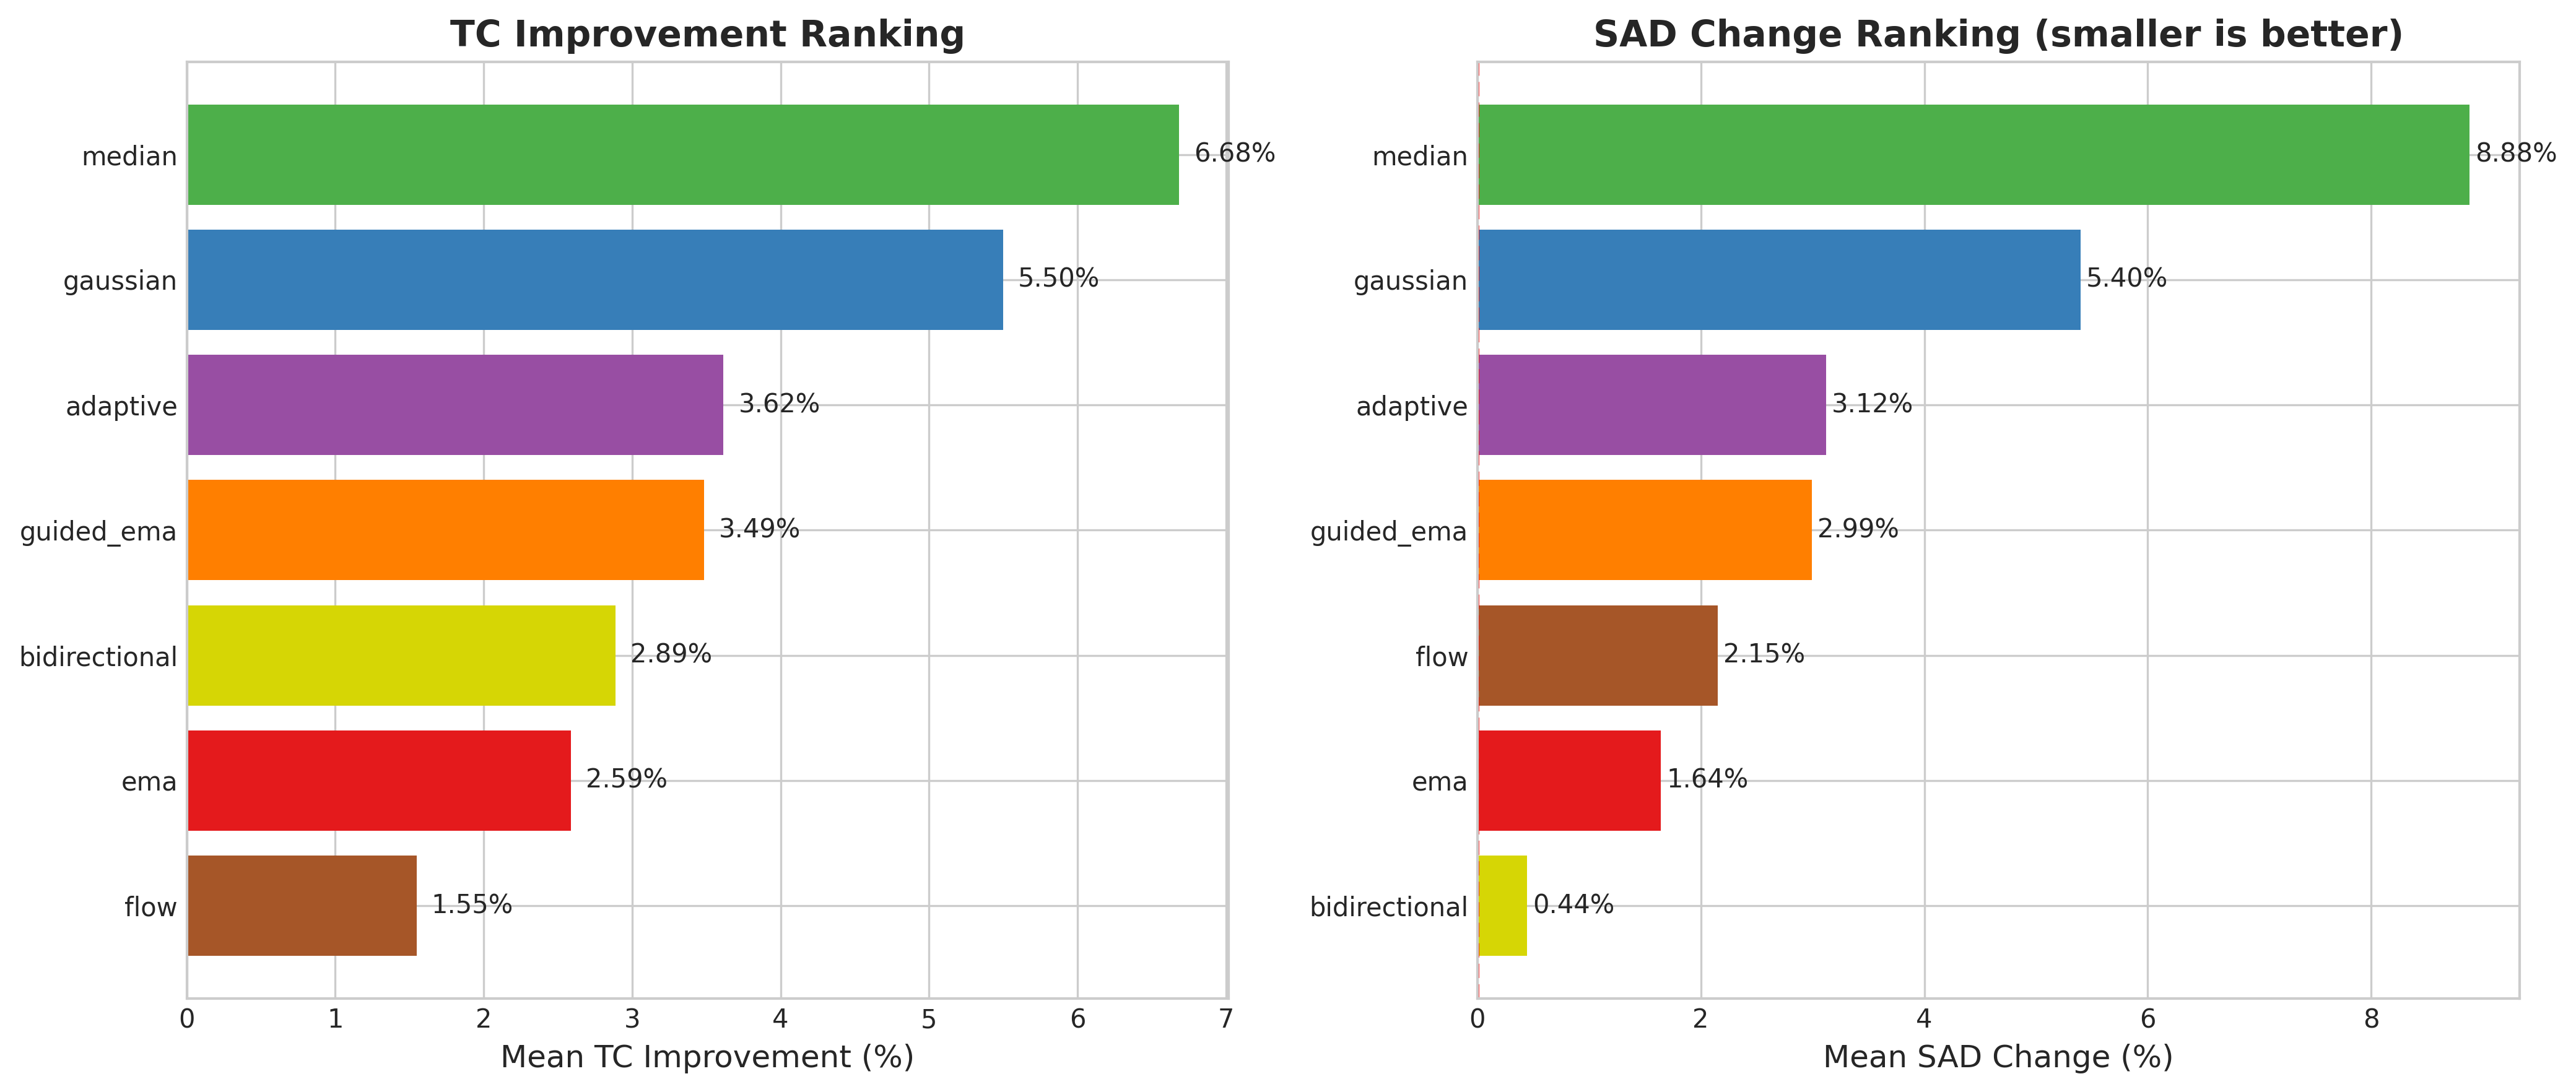
\includegraphics[width=0.95\linewidth]{pic/figure6_performance_ranking.png}
        \vspace{0.1em}
        {\scriptsize TC 提升排名（左）与 SAD 变化排名（右）}
      \end{block}
  \end{columns}
\end{frame}

\begin{frame}[t]{7 种平滑策略性能评估}
  \scriptsize
  \linespread{0.50}\selectfont
  
  \begin{block}{实验设置}
    \scriptsize
    \begin{itemize}
      \setlength{\itemsep}{0.1em}
      \item \textbf{数据集：}YouTubeMatte (10 视频) + VideoMatt (10 视频)，共 20 个测试视频；
      \item \textbf{评估指标：}TC（时序一致性）、SAD（绝对误差和）、MSE、Gradient；
      \item \textbf{方法：}EMA、Gaussian、Median、Adaptive、Guided EMA、Bidirectional、Flow。
    \end{itemize}
  \end{block}
  
  \vspace{0.1em}
  \centering
  \resizebox{0.9\linewidth}{!}{%
  \begin{tabular}{lcccc}
    \toprule
    \textbf{方法} & \textbf{TC 提升 (\%)} & \textbf{SAD 变化 (\%)} & \textbf{MSE 变化 (\%)} & \textbf{细节保留} \\
    \midrule
    Median & 6.68 & +8.88 & +23.91 & Poor \\
    Gaussian & 5.50 & +5.40 & +11.42 & Fair \\
    Adaptive & 3.62 & +3.12 & +5.88 & Fair \\
    Guided EMA & 3.49 & +2.99 & +5.28 & Fair \\
    \textbf{Bidirectional} & \textbf{2.89} & \textbf{+0.44} & \textbf{-0.12} & \textbf{Excellent} \\
    EMA & 2.59 & +1.64 & +2.40 & Good \\
    Flow & 1.55 & +2.15 & +3.62 & Fair \\
    \bottomrule
  \end{tabular}}
  
  
  \vspace{0.1em}
  \notestrip{nankai}{\scriptsize
  \textbf{关键发现：}Bidirectional 是\hilite{唯一能同时改善 TC 和保持精度}的方法，细节保留最佳。
  }
\end{frame}

\begin{frame}[t]{方法对比散点图}
  \scriptsize
  \linespread{0.92}\selectfont
  
  \begin{columns}[T,onlytextwidth]
    \column{0.60\textwidth}
      \centering
      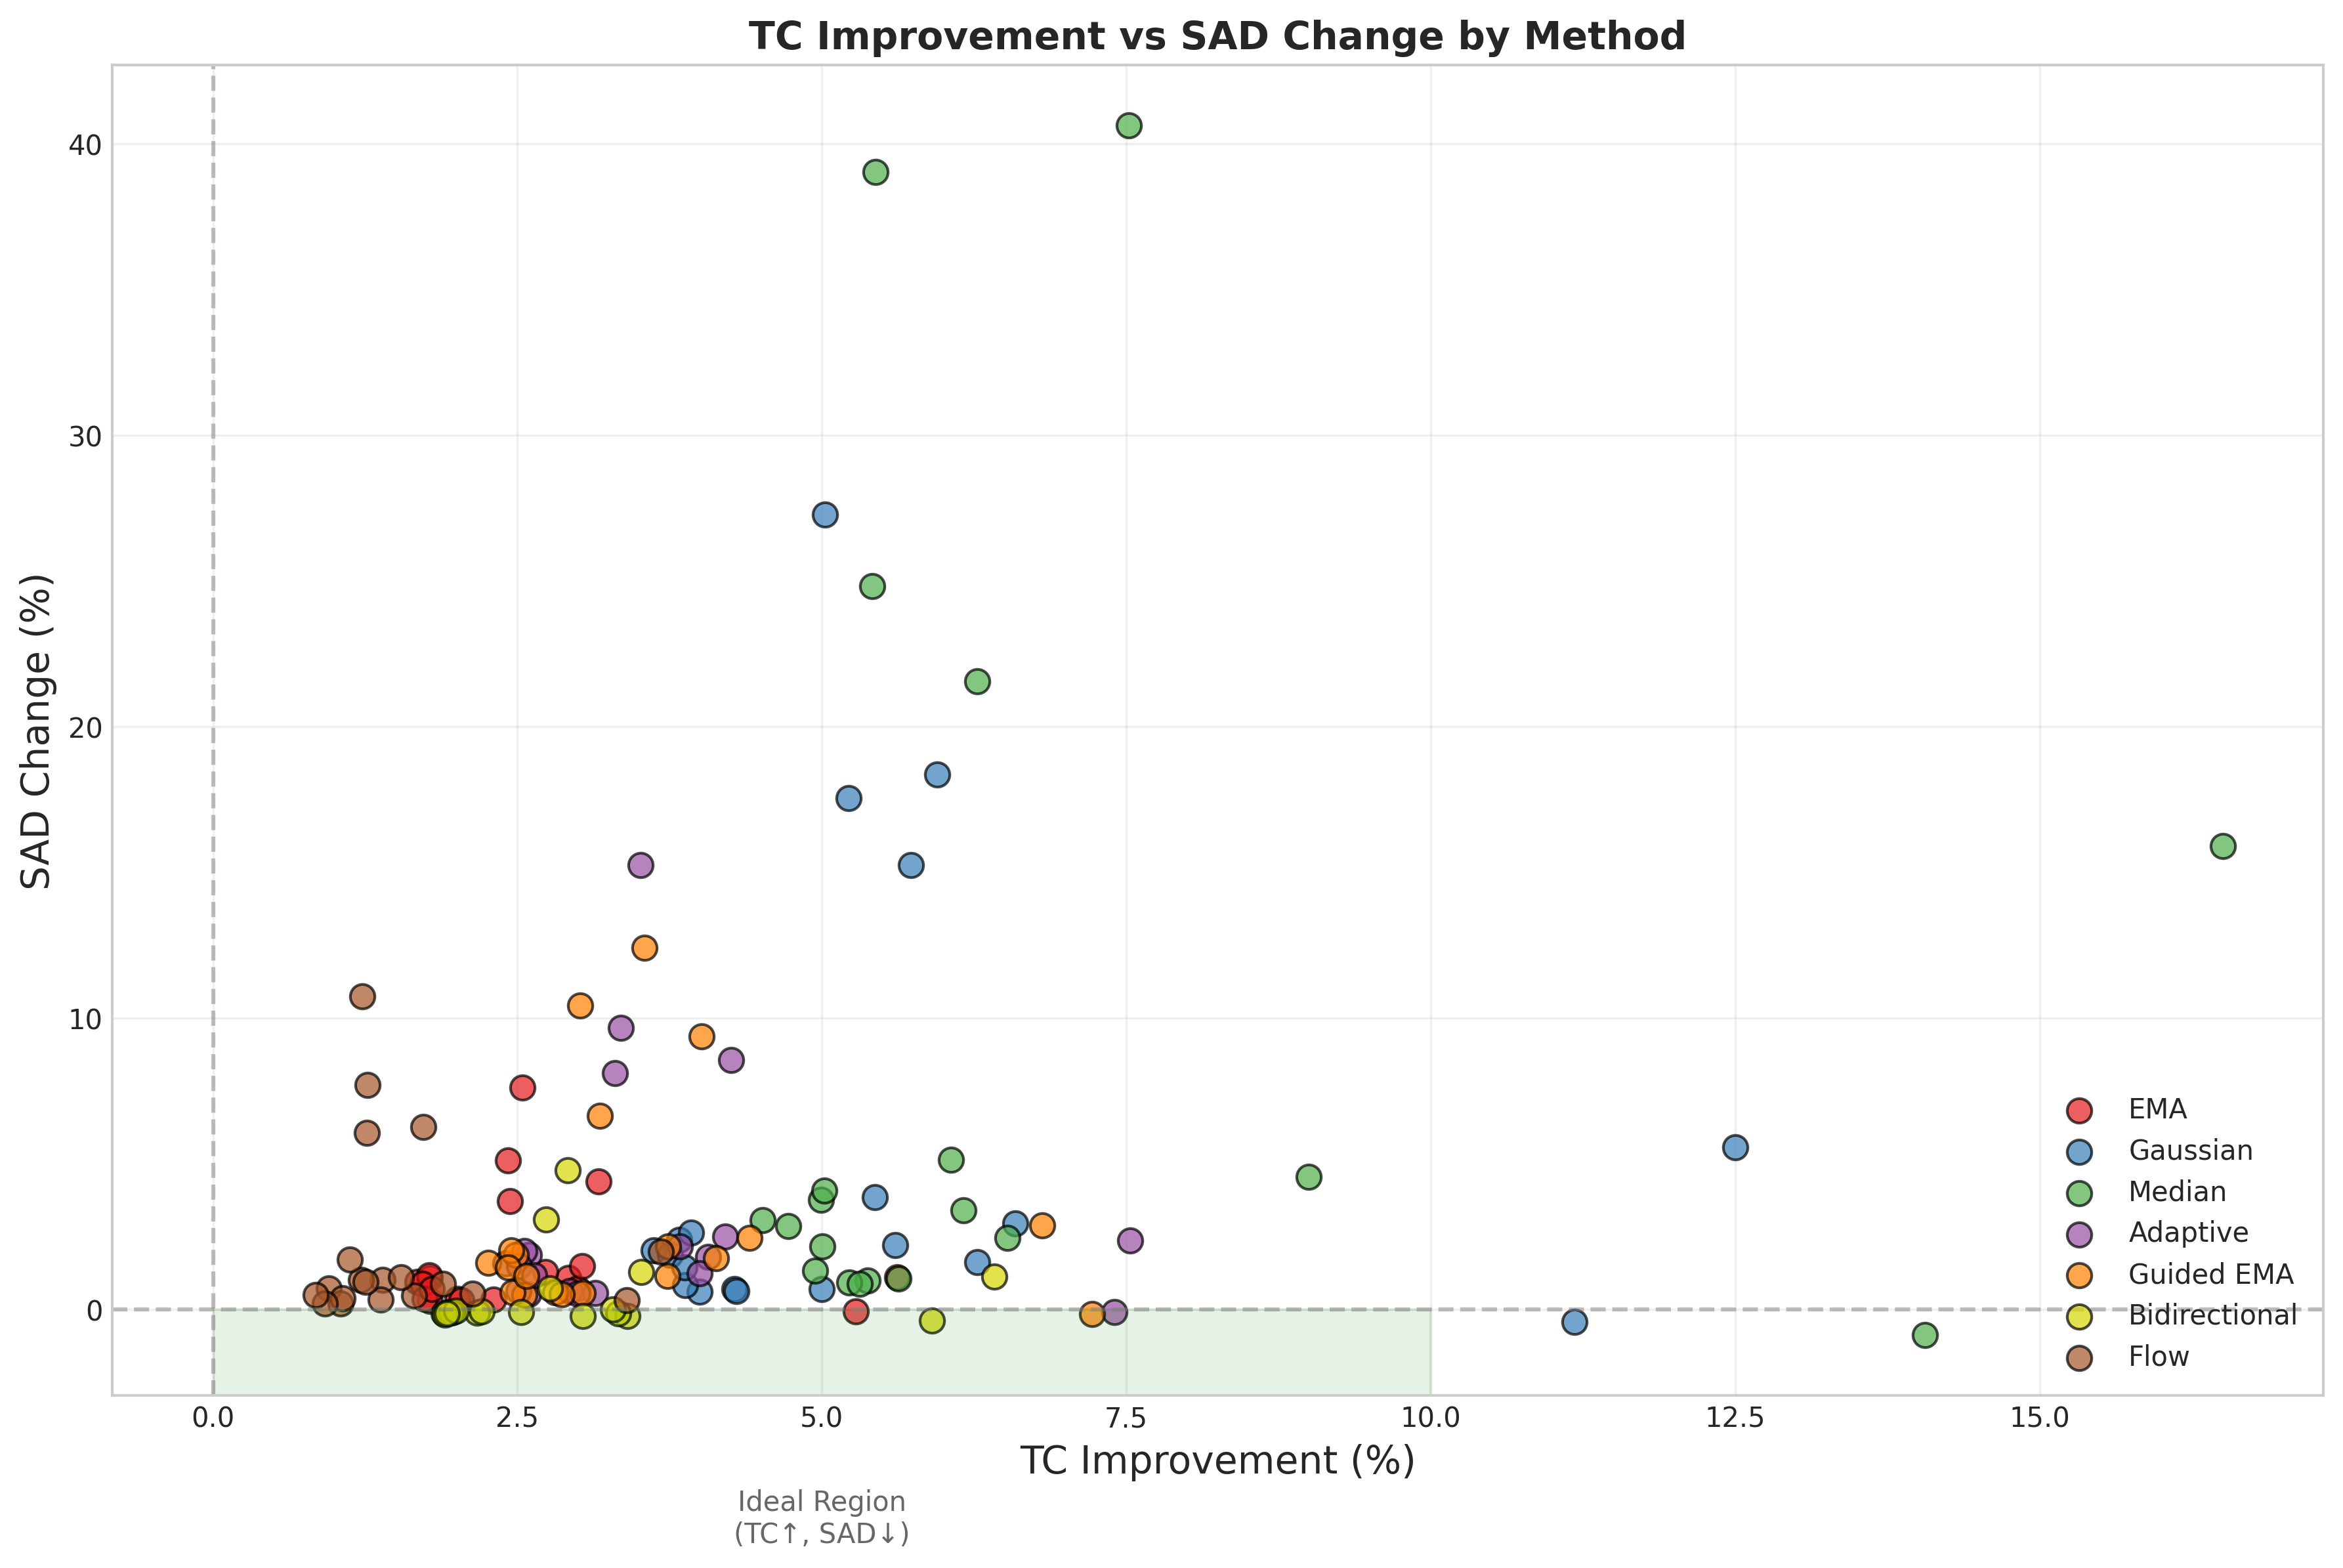
\includegraphics[width=\linewidth]{pic/figure1_tc_vs_sad_scatter.png}
      \vspace{0.1em}
      {\scriptsize  每个点代表一个视频的最佳结果}
      
    \column{0.4\textwidth}
      \begin{block}{解读}
        \begin{itemize}
          \setlength{\itemsep}{0.2em}
          \item 绿色区域：理想方向（TC↑，SAD↓）
          \item \textbf{Bidirectional}：最接近理想区域
          \item Median：TC 提升最大，但 SAD 增加显著
        \end{itemize}
      \end{block}
      
      \vspace{0.3em}
      \begin{block}{最佳参数}
        \scriptsize
        \begin{tabular}{ll}
          \toprule
          \textbf{方法} & \textbf{最佳参数} \\
          \midrule
          Median & window=7 \\
          Gaussian & sigma=2.0, window=7 \\
          \textbf{Bidirectional} & \textbf{alpha=0.7} \\
          \bottomrule
        \end{tabular}
      \end{block}
  \end{columns}
\end{frame}

\begin{frame}[t]{各方法性能分布箱线图}
  \scriptsize
  \linespread{0.98}\selectfont
  
  \begin{columns}[T,onlytextwidth]
    \column{0.7\textwidth}
      \centering
      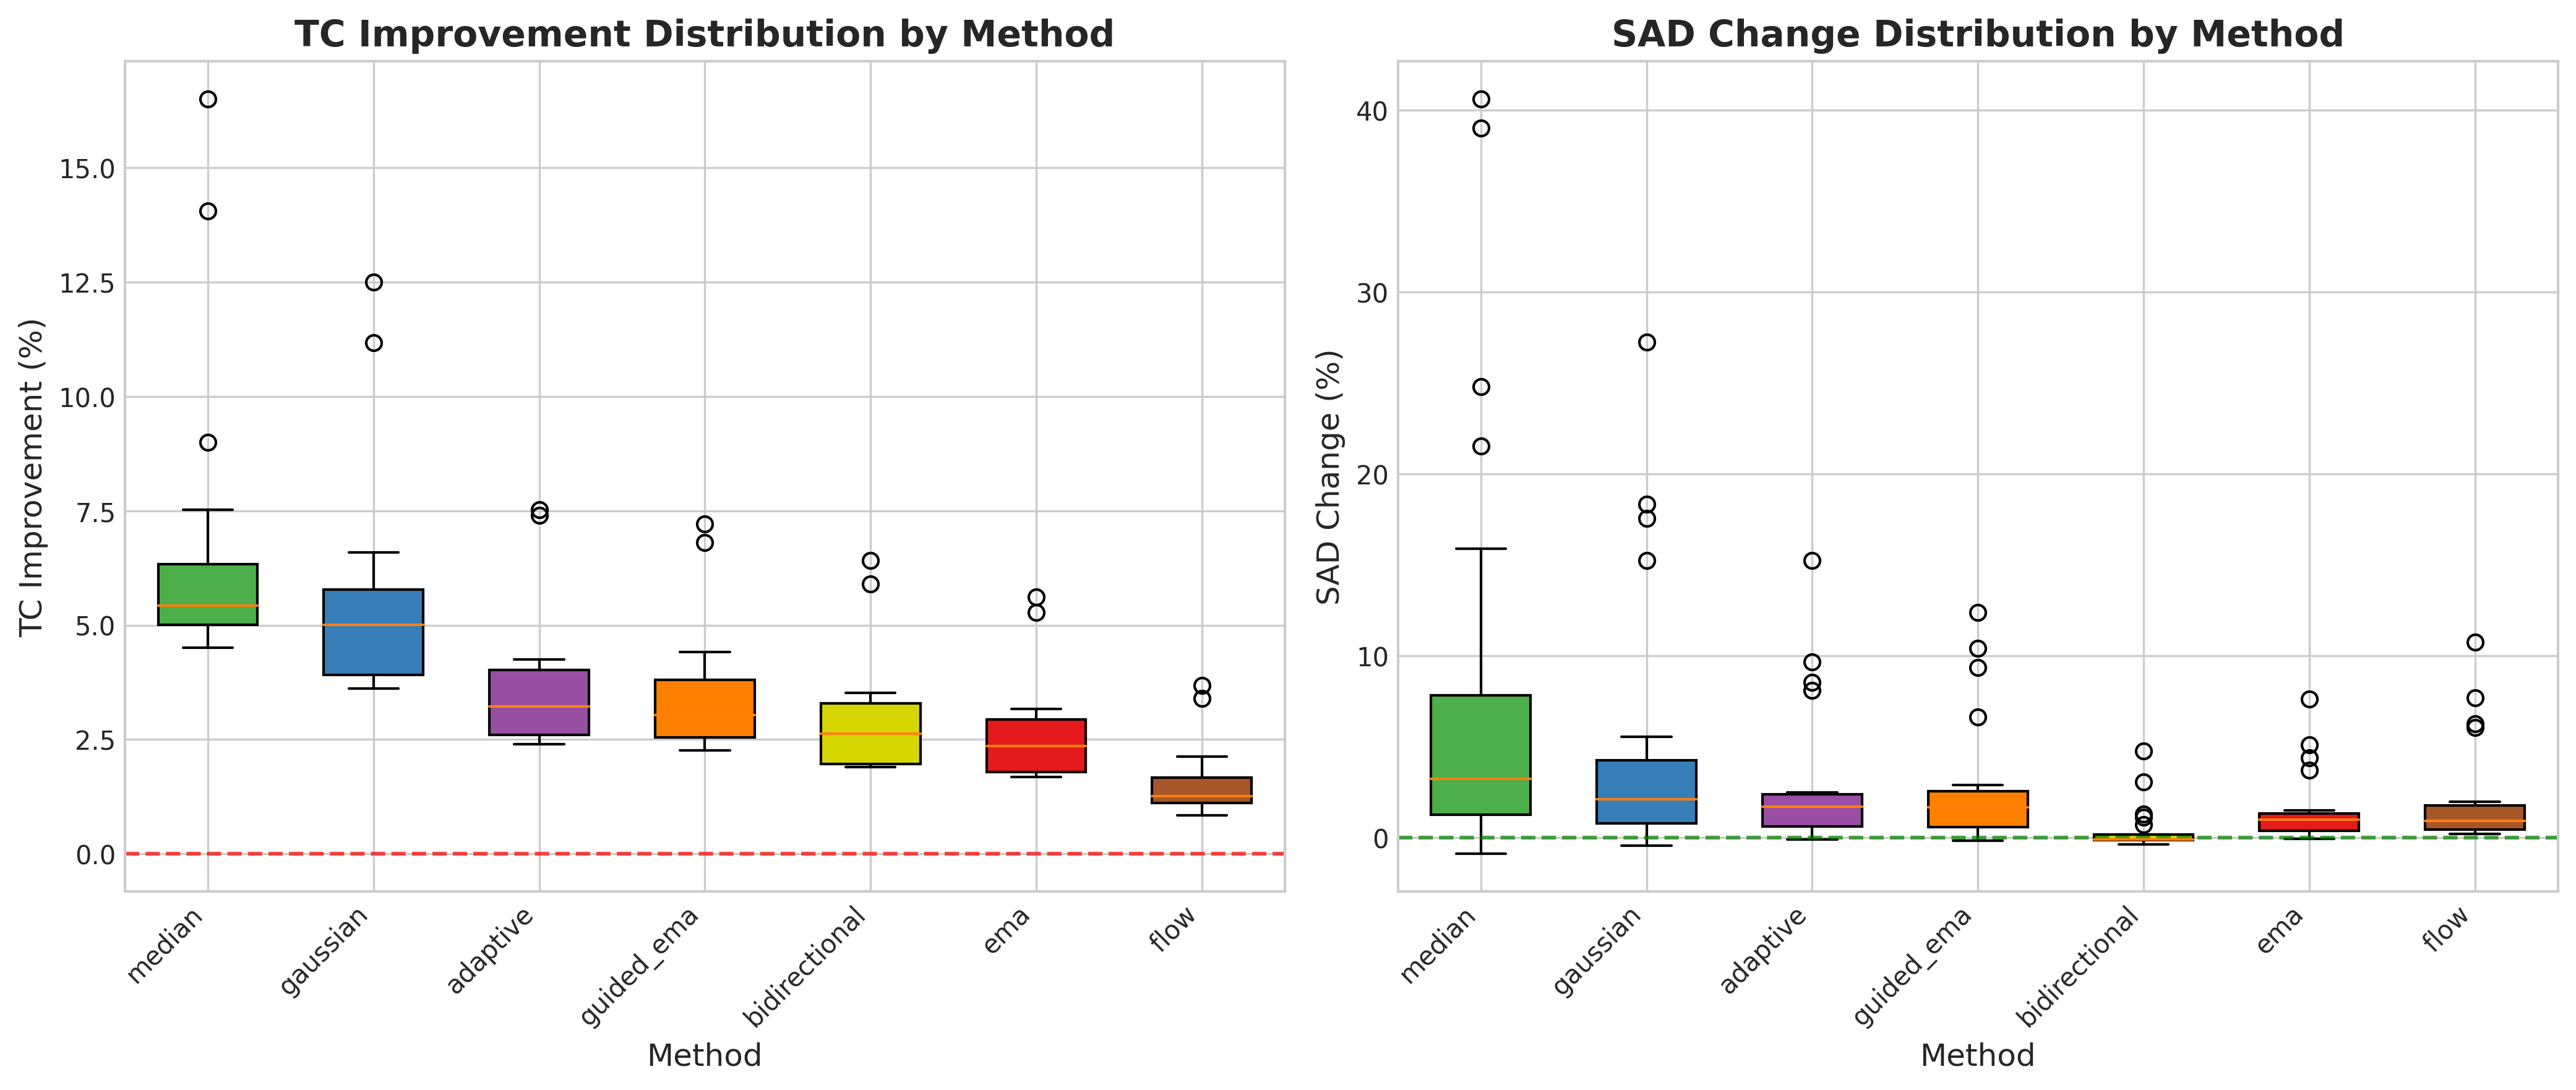
\includegraphics[width=\linewidth]{pic/figure2_method_comparison_boxplot.png}
      \vspace{0.1em}
      {\scriptsize 左：TC 提升分布 \quad | \quad 右：SAD 变化分布}
      
    \column{0.32\textwidth}
      \begin{block}{箱线图解读}
        \begin{itemize}
          \setlength{\itemsep}{0.2em}
          \item 箱体 = 四分位距（50\% 数据）
          \item 横线 = 中位数
          \item 圆形 = 异常值
        \end{itemize}
      \end{block}
      
      \vspace{0.3em}
      \begin{block}{关键观察}
        \begin{itemize}
          \setlength{\itemsep}{0.2em}
          \item \textbf{Bidirectional}：SAD 分布最集中，异常值最少
          \item \textbf{Median}：TC 提升高但波动大
          \item \textbf{Gaussian}：TC 提升分布较稳定
        \end{itemize}
      \end{block}
  \end{columns}
  
  \vspace{0.1em}
  \notestrip{nankai}{\scriptsize
  \textbf{结论：}Bidirectional 的 SAD 变化分布最集中，说明其精度表现\hilite{最稳定}，不同视频间差异最小。
  }
\end{frame}

\begin{frame}[t]{Bidirectional 平滑效果对比}
  \scriptsize
  \linespread{0.98}\selectfont
  
  \begin{columns}[T,onlytextwidth]
    \column{0.55\textwidth}
      \centering
      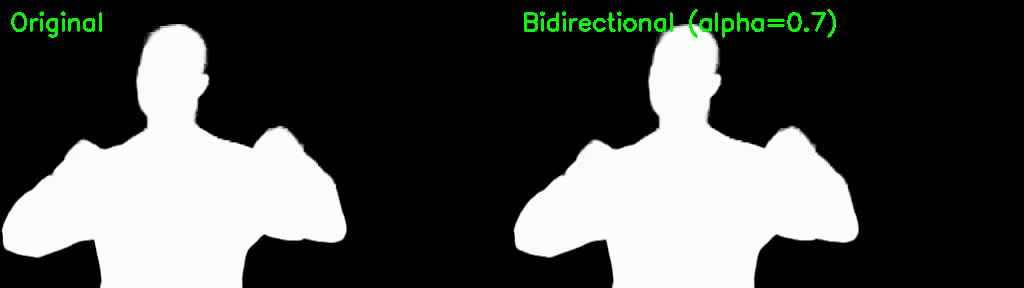
\includegraphics[width=0.98\linewidth]{pic/gif_frames/frame_0001.png}
      \vspace{0.1em}
      {\tiny 左：原始 alpha \quad | \quad 右：Bidirectional 平滑后}
      
      \vspace{0.2em}
      \href{run:pic/youtubematte_motion_0016_bidirectional_comparison_slow_hq.gif}{%
        \color{accentblue}{\underline{[Click] 点击播放动画效果 (GIF)}}%
      }
      
      \vspace{0.3em}
      \begin{block}{视觉效果}
        \begin{itemize}
          \setlength{\itemsep}{0.2em}
          \item 发丝细节\hilite{无明显模糊}
          \item 边缘抖动\hilite{明显减弱}
          \item 背景替换后\hilite{闪烁减少}
        \end{itemize}
      \end{block}
      
    \column{0.42\textwidth}
      \begin{block}{性能指标}
        \scriptsize
        \begin{tabular}{lcc}
          \toprule
          \textbf{指标} & \textbf{数值} & \textbf{评价} \\
          \midrule
          TC 提升 & 2.89\% & 提升 \\
          SAD 变化 & +0.44\% & 几乎无损 \\
          MSE 变化 & -0.12\% & 改善 \\
          \bottomrule
        \end{tabular}
      \end{block}
      
      \vspace{0.3em}
      \begin{block}{优劣分析}
        \scriptsize
        \begin{itemize}
          \setlength{\itemsep}{0.1em}
          \item \textbf{优点：}精度几乎无损，发丝细节保留完整
          \item \textbf{缺点：}TC 提升幅度相对较小
        \end{itemize}
      \end{block}
  \end{columns}
  
  \vspace{0.2em}
  \notestrip{softgreen}{\scriptsize
  \textbf{结论：}Bidirectional 在\hilite{保持视觉质量的同时}实现时序一致性提升，是精度无损场景的最佳选择。
  }
\end{frame}

\begin{frame}[t]{Median 平滑效果对比}
  \scriptsize
  \linespread{0.98}\selectfont
  
  \begin{columns}[T,onlytextwidth]
    \column{0.55\textwidth}
      \centering
      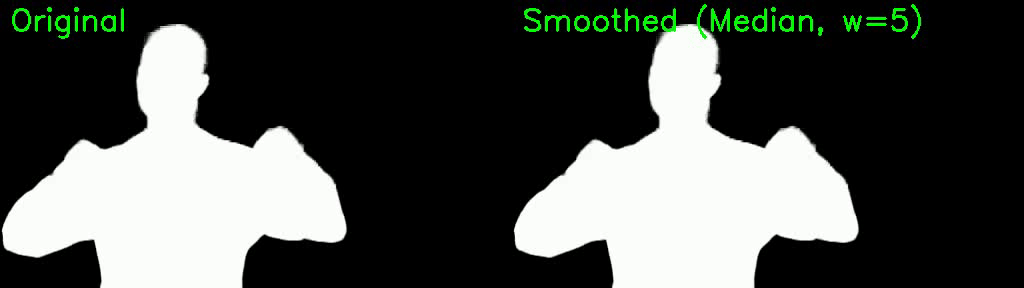
\includegraphics[width=0.98\linewidth]{pic/median_frames/median_frame_0001.png}
      \vspace{0.1em}
      {\tiny 左：原始 alpha \quad | \quad 右：Median 平滑后}
      
      \vspace{0.2em}
      \href{run:pic/youtubematte_motion_0016_comparison_slow_hq.gif}{%
        \color{accentblue}{\underline{[Click] 点击播放动画效果 (GIF)}}%
      }
      
      \vspace{0.3em}
      \begin{block}{视觉效果}
        \begin{itemize}
          \setlength{\itemsep}{0.2em}
          \item 发丝细节\hilite{明显模糊}
          \item 边缘抖动\hilite{减少但细节丢失}
          \item 背景替换后\hilite{毛边明显}
        \end{itemize}
      \end{block}
      
    \column{0.42\textwidth}
      \begin{block}{性能指标}
        \scriptsize
        \begin{tabular}{lcc}
          \toprule
          \textbf{指标} & \textbf{数值} & \textbf{评价} \\
          \midrule
          TC 提升 & 6.68\% & 提升最大 \\
          SAD 变化 & +8.88\% & 恶化严重 \\
          MSE 变化 & +23.91\% & 恶化严重 \\
          \bottomrule
        \end{tabular}
      \end{block}
      
      \vspace{0.3em}
      \begin{block}{优劣分析}
        \scriptsize
        \begin{itemize}
          \setlength{\itemsep}{0.1em}
          \item \textbf{优点：}TC 提升最大（6.68\%），时序稳定性最好
          \item \textbf{缺点：}发丝模糊严重，视觉损失不可接受
        \end{itemize}
      \end{block}
  \end{columns}
  
  \vspace{0.2em}
  \notestrip{softorange}{\scriptsize
  \textbf{结论：}Median 数值最优但\hilite{视觉损失严重}，不适合需要精细边缘的实际应用。
  }
\end{frame}


\begin{frame}[t]{Gaussian 平滑效果对比}
  \scriptsize
  \linespread{0.98}\selectfont
  
  \begin{columns}[T,onlytextwidth]
    \column{0.55\textwidth}
      \centering
      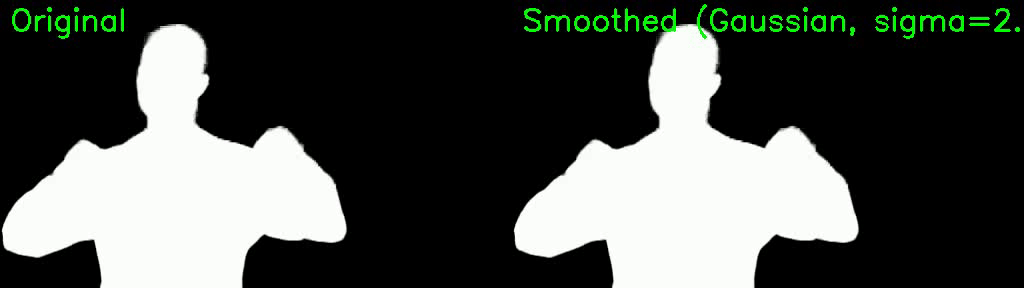
\includegraphics[width=0.98\linewidth]{pic/gaussian_frames/gaussian_frame_0001.png}
      \vspace{0.1em}
      {\tiny 左：原始 alpha \quad | \quad 右：Gaussian 平滑后 (sigma=2.0)}
      
      \vspace{0.2em}
      \href{run:pic/youtubematte_motion_0016_gaussian_comparison_slow_hq.gif}{%
        \color{accentblue}{\underline{[Click] 点击播放动画效果 (GIF)}}%
      }
      
      \vspace{0.3em}
      \begin{block}{视觉效果}
        \begin{itemize}
          \setlength{\itemsep}{0.2em}
          \item 发丝细节\hilite{轻微模糊}
          \item 边缘抖动\hilite{明显减少}
          \item 整体\hilite{平衡性较好}
        \end{itemize}
      \end{block}
      
    \column{0.42\textwidth}
      \begin{block}{性能指标}
        \scriptsize
        \begin{tabular}{lcc}
          \toprule
          \textbf{指标} & \textbf{数值} & \textbf{评价} \\
          \midrule
          TC 提升 & 4.0\% & 提升显著 \\
          SAD 变化 & +2.4\% & 轻微恶化 \\
          MSE 变化 & +3.0\% & 轻微恶化 \\
          \bottomrule
        \end{tabular}
      \end{block}
      
      \vspace{0.3em}
      \begin{block}{优劣分析}
        \scriptsize
        \begin{itemize}
          \setlength{\itemsep}{0.1em}
          \item \textbf{优点：}TC 提升显著（4.0\%），是 TC 和精度的最佳平衡点
          \item \textbf{缺点：}发丝有轻微模糊，精度略有下降
        \end{itemize}
      \end{block}
  \end{columns}
  
  \vspace{0.2em}
  \notestrip{accentblue}{\scriptsize
  \textbf{建议：}追求平衡可选 Gaussian (sigma=2.0, window=5)；追求精度无损可选 Bidirectional (alpha=0.7)。
  }
\end{frame}


\begin{frame}[t]{两个数据集上的性能对比}
  \scriptsize
  \linespread{0.98}\selectfont
  
  \begin{columns}[T,onlytextwidth]
    \column{0.7\textwidth}
      \centering
      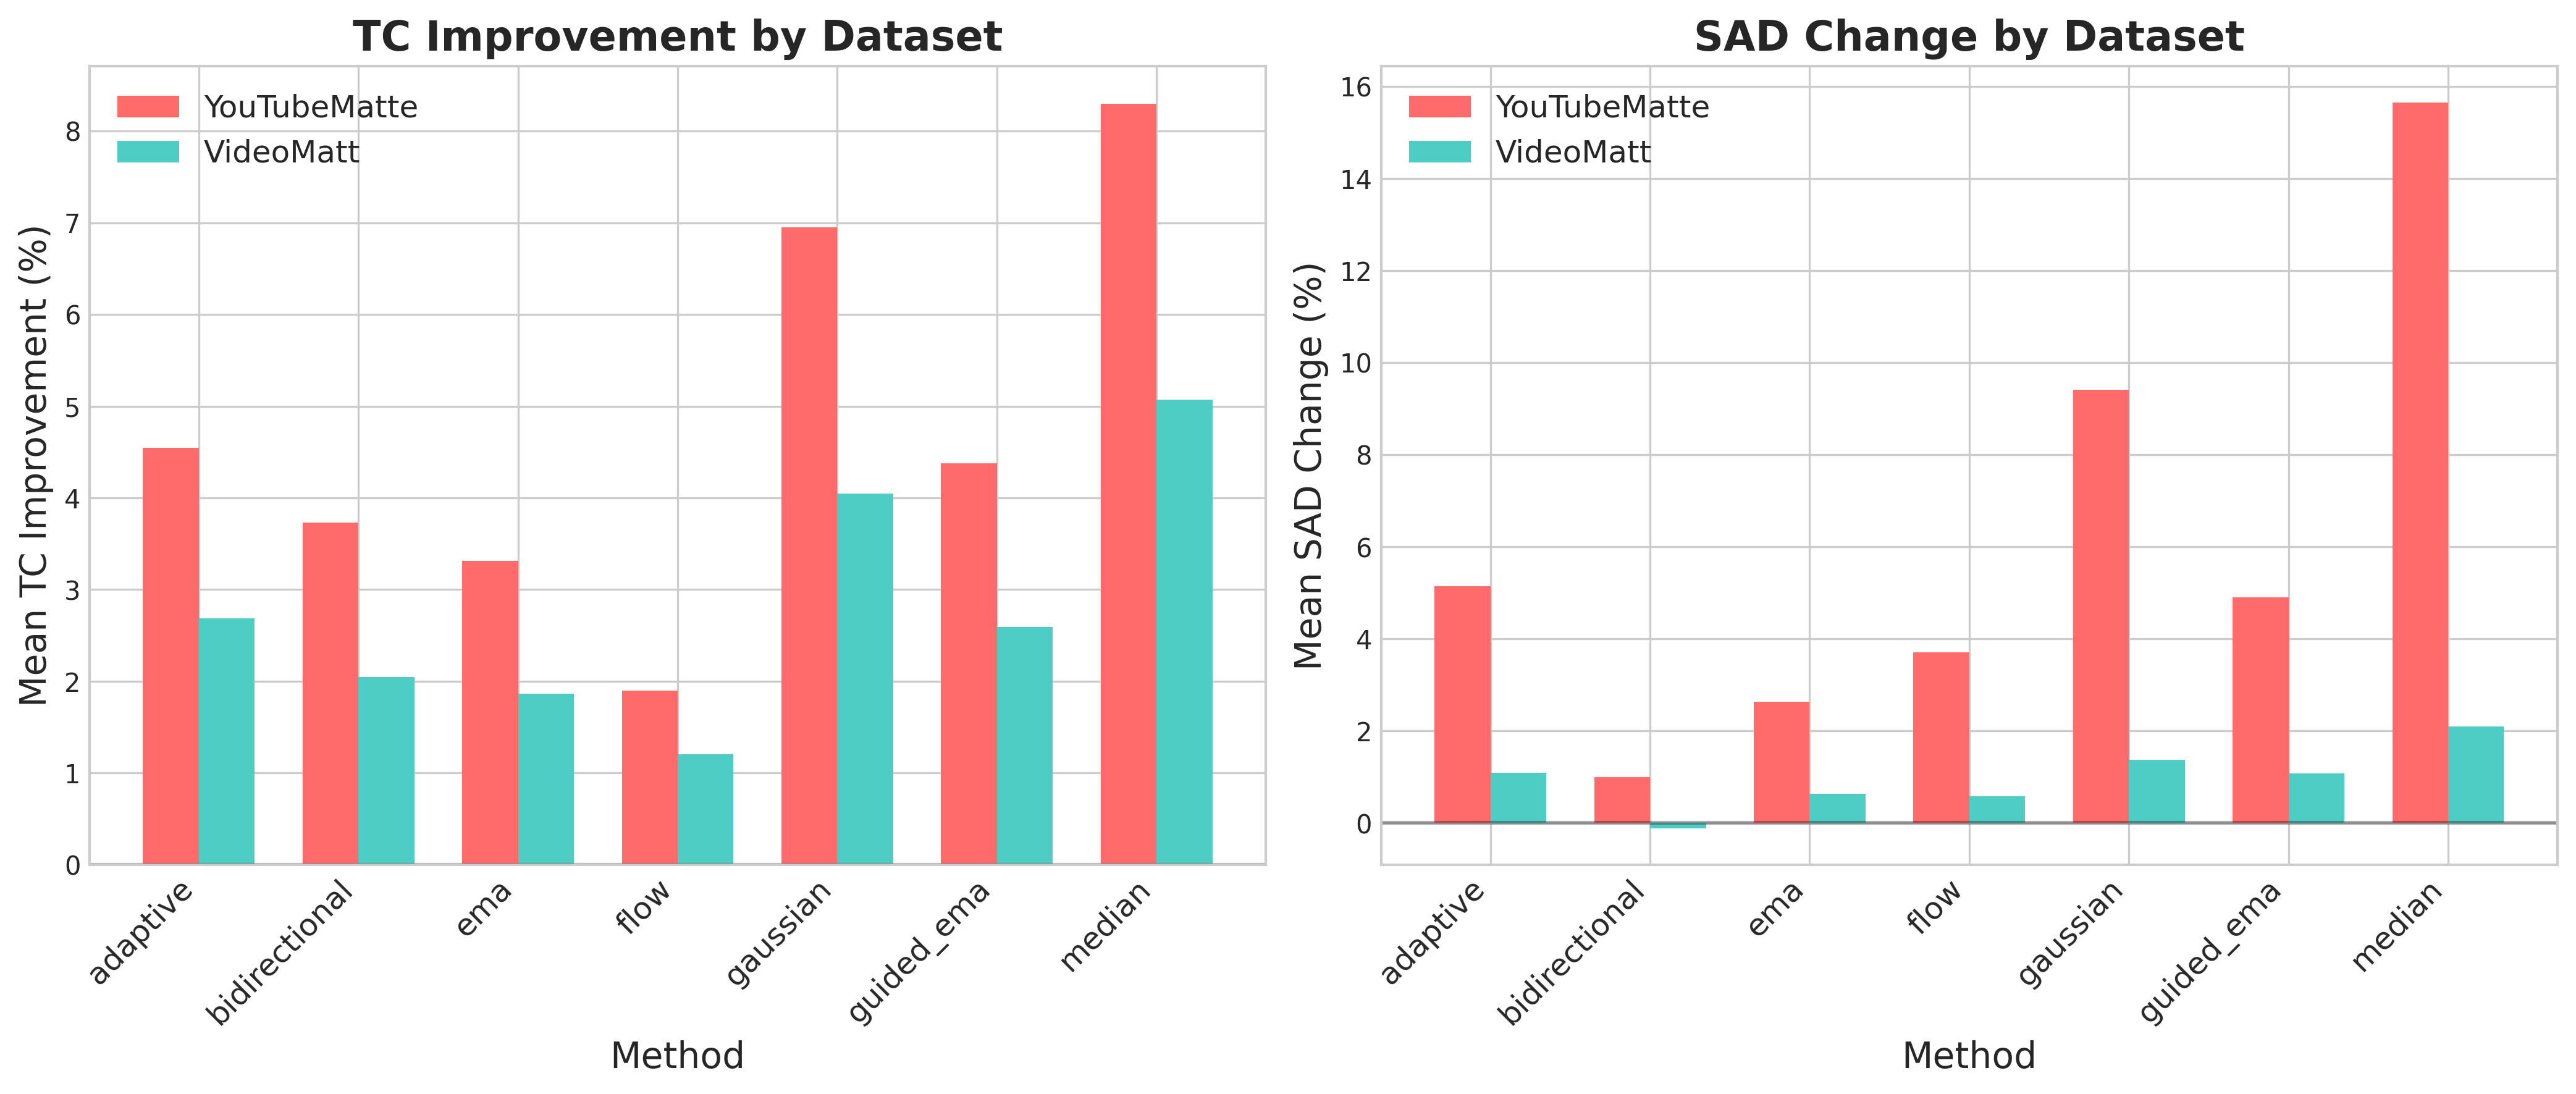
\includegraphics[width=0.98\linewidth]{pic/figure3_dataset_comparison.png}
      \vspace{0.1em}
      {\scriptsize 左：TC 提升对比 \quad | \quad 右：SAD 变化对比}
      
    \column{0.32\textwidth}
      \begin{block}{关键观察}
        \begin{itemize}
          \setlength{\itemsep}{0.2em}
          \item YouTubeMatte 上效果\hilite{普遍更好}
          \item VideoMatt 更具挑战性
          \item \textbf{Bidirectional} 表现\hilite{最稳定}
        \end{itemize}
      \end{block}
      
      \vspace{0.5em}
      \begin{block}{差异分析}
        \scriptsize
        VideoMatt 包含更多\hilite{复杂运动}和\hilite{精细结构}，平滑难度更高。
      \end{block}
    \end{columns}
   \vspace{0.1em}
  \notestrip{accentblue}{\scriptsize
  \textbf{结论：}Bidirectional 在两个数据集上表现最稳定，适合不同场景的视频抠图任务。
  }
\end{frame}

\begin{frame}[t]{Gaussian 参数敏感性分析}
  \vspace{-0.5cm}
  \scriptsize
  \linespread{0.98}\selectfont
  
  \begin{columns}[T,onlytextwidth]
    \column{0.65\textwidth}
      \centering
      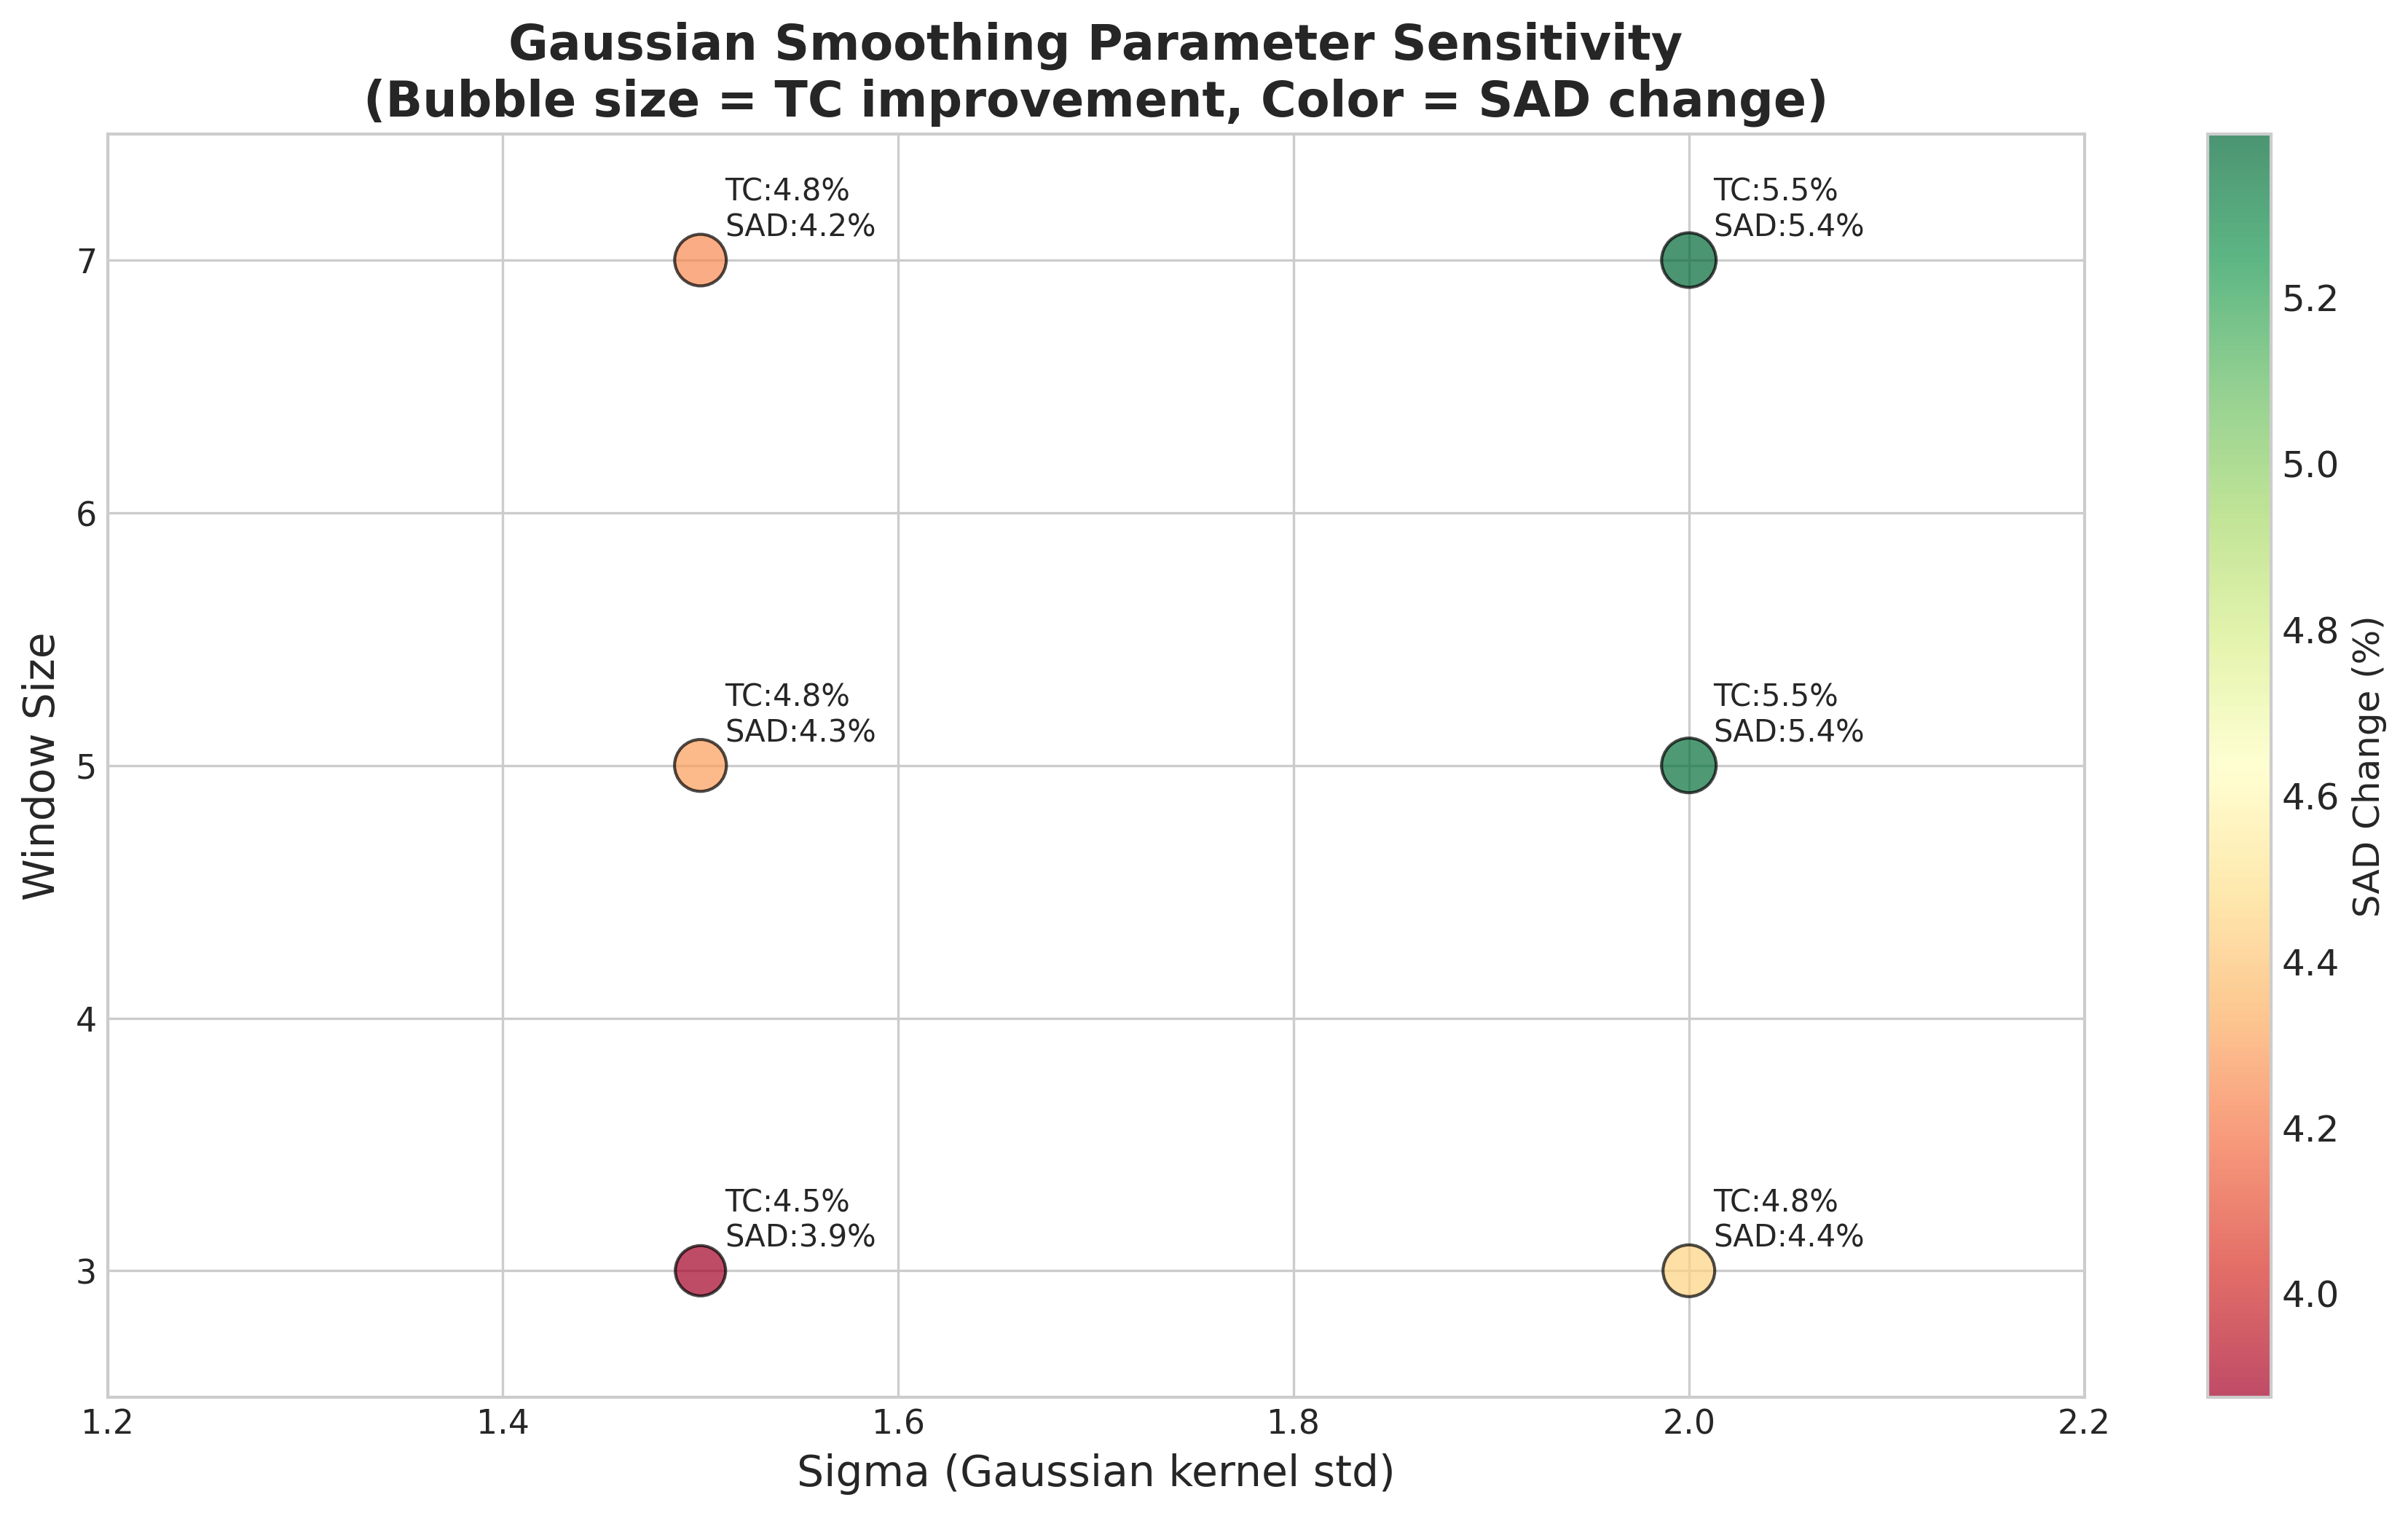
\includegraphics[width=0.98\linewidth]{pic/figure4_gaussian_parameter_sensitivity.png}
      \vspace{0.1em}
      {\scriptsize 气泡大小 = TC 提升，颜色 = SAD 变化}
      
    \column{0.32\textwidth}
      \begin{block}{参数趋势}
        \begin{itemize}
          \setlength{\itemsep}{0.2em}
          \item 增大 sigma → TC 提升增加
          \item 增大 sigma → SAD 恶化加剧
          \item 增大窗口 → 效果饱和
        \end{itemize}
      \end{block}
      
      \vspace{0.3em}
      \begin{block}{推荐参数}
        \centering
        \metricchip{softgreen}{sigma=2.0}{window=5} \\
        \vspace{0.1em}
        {\scriptsize TC 提升: 4.0\%, SAD 增加: 2.4\%}
      \end{block}
  \end{columns}
  
  \vspace{0.1em}
  \notestrip{accentblue}{\scriptsize
  \textbf{建议：}追求平衡可选 Gaussian；追求精度无损可选 Bidirectional。
  }
\end{frame}

\begin{frame}[t]{综合性能雷达图}
  \vspace{-0.5cm}
  \scriptsize
  \linespread{0.98}\selectfont
  
  \begin{columns}[T,onlytextwidth]
    \column{0.60\textwidth}
      \centering
      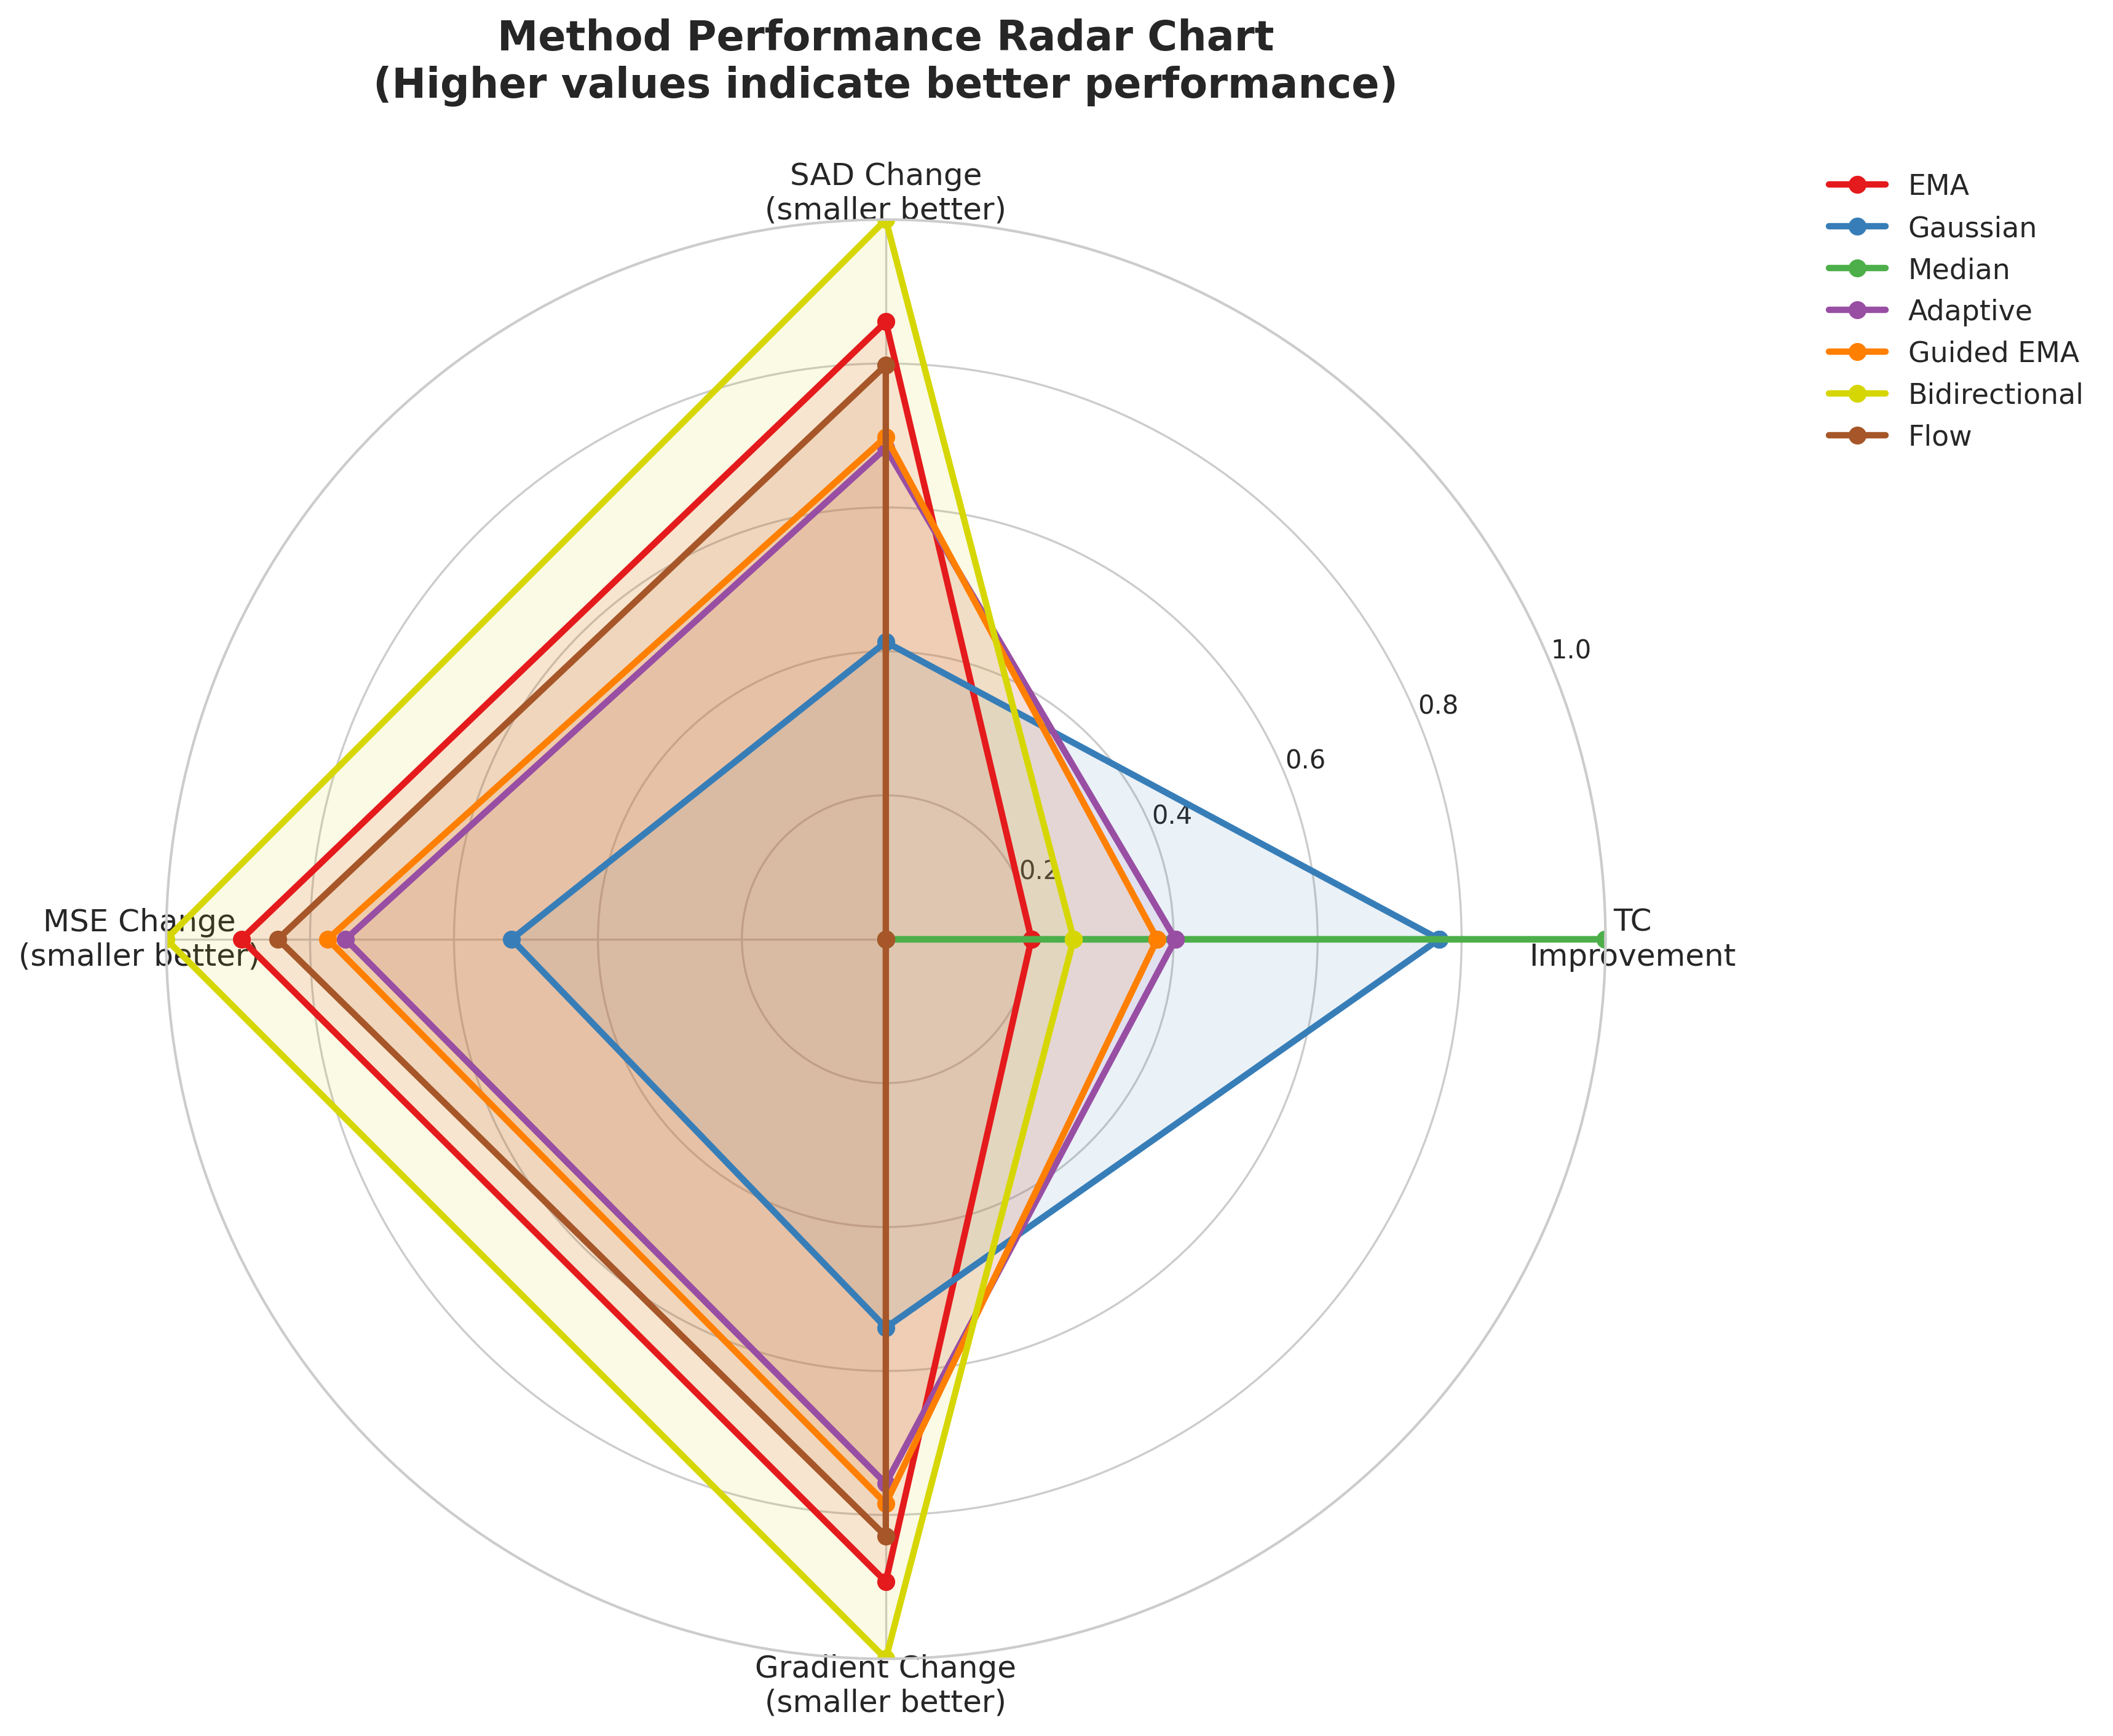
\includegraphics[width=0.95\linewidth]{pic/figure5_radar_chart.png}
      
    \column{0.32\textwidth}
      \begin{block}{解读}
        \begin{itemize}
          \setlength{\itemsep}{0.2em}
          \item 雷达图中 SAD/MSE/Gradient 已反向归一化，\hilite{值越大 = 性能越好}。
          \item \textbf{Bidirectional} 最均衡
          \item Median 偏科严重
        \end{itemize}
      \end{block}
      
      \vspace{0.3em}
      \begin{block}{总结}
        \centering
        \textbf{Bidirectional (alpha=0.7)} \\
        \vspace{0.1em}
        → 雷达图面积最大 \\
        → 推荐为默认平滑策略
      \end{block}
  \end{columns}
  
  
\end{frame}

\begin{frame}[t]{视频换背景 Demo}
  \scriptsize
  \linespread{0.98}\selectfont
  
  \begin{columns}[T,onlytextwidth]
    \column{0.48\textwidth}
      \begin{block}{平滑后 alpha 对比}
        \centering
        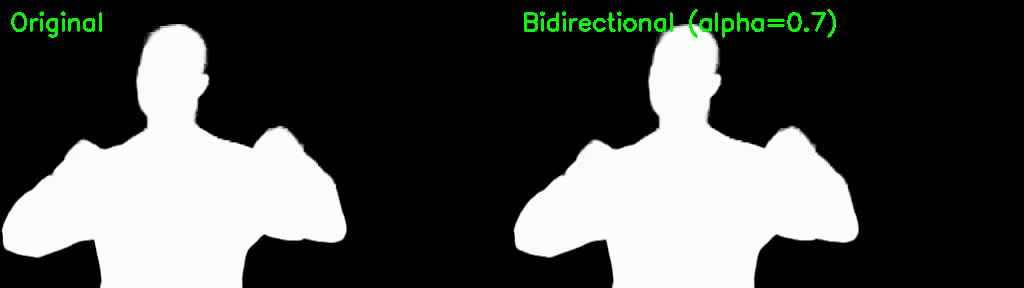
\includegraphics[width=0.95\linewidth]{pic/gif_frames/frame_0001.png}
        \vspace{0.1em}
        {\scriptsize 左：原始 \quad | \quad 右：Bidirectional 平滑后}
        
        \vspace{0.2em}
        \href{run:pic/youtubematte_motion_0016_bidirectional_slow_hq.gif}{%
          \color{accentblue}{\underline{[Click] 播放动画效果 (GIF)}}%
        }
      \end{block}
      
    \column{0.48\textwidth}
      \begin{block}{换背景效果}
        \centering
        
\includegraphics[width=0.35\linewidth]{pic/background.jpg}
        \vspace{0.1em}
        \\
        {\scriptsize 平滑后 alpha → RGBA → 背景替换}
        
        \vspace{0.2em}
        \href{run:pic/youtubematte_motion_0016_bidirectional_composer.mp4}{%
          \color{accentblue}{\underline{[Click] 播放换背景动画 (mp4)}}%
        }
      \end{block}
  \end{columns}
  
  \vspace{0.2em}
  \begin{block}{接口说明}
    \scriptsize
    \textbf{输入：}图像主线首帧 alpha / mask
    \textbf{处理：}MatAnyone2 + Bidirectional 时序平滑 (alpha=0.7)
    \textbf{输出：}逐帧稳定 alpha + 换背景合成视频
  \end{block}
  
  \vspace{0.1em}
  \notestrip{softgreen}{\scriptsize
  \textbf{效果：}Bidirectional 平滑后，背景替换视频的\hilite{边界闪烁明显减少}，同时\hilite{发丝细节保持清晰}。
  }
\end{frame}

\section{参考资料}
\begin{frame}[t]{参考资料}
  \footnotesize
  \linespread{0.94}\selectfont
  \begin{columns}[T,onlytextwidth]
    \column{0.52\textwidth}
      {\color{nankai}\bfseries 目标定位与分割}\par
      \vspace{0.12em}
      {\footnotesize
      \raggedright
      \begin{itemize}
        \setlength{\itemsep}{0.16em}
        \item[\textcolor{nankai}{[1]}] Feichtenhofer \textit{et al.}, ``Segment Anything in Images and Videos,'' 2024.
        \item[\textcolor{nankai}{[2]}] Feichtenhofer \textit{et al.}, ``SAM 3: Segment Anything with Concepts,'' 2025.
        \item[\textcolor{nankai}{[3]}] Ren \textit{et al.}, ``Grounded SAM: Assembling Open-World Models for Diverse Visual Tasks,'' 2024.
        \item[\textcolor{nankai}{[4]}] IDEA Research, ``Grounded-SAM-2,'' GitHub repository, 2024.
      \end{itemize}}
    \column{0.48\textwidth}
      {\color{nankai}\bfseries Matting 与视频}\par
      \vspace{0.12em}
      {\footnotesize
      \raggedright
      \begin{itemize}
        \setlength{\itemsep}{0.14em}
        \item[\textcolor{nankai}{[5]}] Kim \textit{et al.}, ``\textbf{ZIM: Zero-Shot Image Matting for Anything},'' ICCV, 2025.\; {\scriptsize（本工作的精细抠图基座）}
        \item[\textcolor{nankai}{[6]}] Li, Jain, and Shi, ``Matting Anything,'' 2023.
        \item[\textcolor{nankai}{[7]}] Yang \textit{et al.}, ``MatAnyone 2: Scaling Video Matting via a Learned Quality Evaluator,'' 2026.
      \end{itemize}}

      \vspace{0.10em}
      {\color{nankai}\bfseries 边界优化与应用}\par
      \vspace{0.12em}
      {\footnotesize
      \raggedright
      \begin{itemize}
        \setlength{\itemsep}{0.14em}
        \item[\textcolor{nankai}{[8]}] He, Sun, and Tang, ``Guided Image Filtering,'' ECCV, 2010.
        \item[\textcolor{nankai}{[9]}] Hugging Face, ``Diffusers Documentation: Inpainting,'' Documentation, 2025.
      \end{itemize}}

  \end{columns}
\end{frame}

\end{document}
